\documentclass[11pt]{article}
\usepackage[T1]{fontenc}
\usepackage{lmodern}
\input{glyphtounicode}
\input{glyphtounicode-cmex}
\pdfgentounicode=1
\usepackage[margin=1in]{geometry}
\usepackage{amsmath,amssymb,amsthm,mathtools}
\usepackage{microtype}
\usepackage{booktabs,array,enumitem}
\usepackage{tikz}
\usetikzlibrary{arrows.meta,calc,patterns,positioning,decorations.pathreplacing}
\usepackage{xurl}
\usepackage[colorlinks=true,linkcolor=blue!50!black,citecolor=blue!50!black,urlcolor=blue!50!black,hypertexnames=false]{hyperref}
\pdfinfoomitdate=1
\pdftrailerid{}
\pdfsuppressptexinfo=15
\setlength{\emergencystretch}{2em}
\setcounter{tocdepth}{2}
\numberwithin{equation}{section}
\newtheorem{theorem}{Theorem}[section]
\newtheorem{proposition}[theorem]{Proposition}
\newtheorem{lemma}[theorem]{Lemma}
\newtheorem{corollary}[theorem]{Corollary}
\theoremstyle{definition}
\newtheorem{definition}[theorem]{Definition}
\theoremstyle{remark}
\newtheorem{remark}[theorem]{Remark}
\DeclareMathOperator{\Tr}{Tr}
\DeclareMathOperator{\rank}{rank}
\DeclareMathOperator{\dist}{dist}
\DeclareMathOperator{\diam}{diam}
\DeclareMathOperator{\supp}{supp}
\DeclareMathOperator{\id}{id}
\newcommand{\norm}[1]{\lVert #1\rVert}
\newcommand{\abs}[1]{\lvert #1\rvert}
\title{Polynomial PEPS approximation of gapped\texorpdfstring{\\}{ }square-grid ground states}
\author{OpenAI}
\date{September 24, 2026}
\hypersetup{pdftitle={Polynomial PEPS approximation of gapped square-grid ground states},pdfauthor={OpenAI}}
\begin{document}
\maketitle
\begin{abstract}
We prove that the unique ground state of a uniformly gapped nearest-neighbor
Hamiltonian on an $L\times L$ square lattice admits a projected entangled-pair
state approximation with bond dimension polynomial in $L$ and global vector
error at most $L^{-1}$ after normalization. Only the gap of the full Hamiltonian is assumed.
The result is an existence theorem, with constants uniform over
Hamiltonians of fixed local dimension, interaction strength, and gap.
\end{abstract}
\tableofcontents
\clearpage
\section{Introduction}\label{sec:introduction}

A projected entangled-pair state (PEPS) represents a many-body vector by local
tensors joined along the edges of its interaction lattice. The central
approximation question is whether ground states of gapped local Hamiltonians
admit such representations with modest virtual dimensions. An entropy area
law controls every bipartite cut, but a global vector approximation requires
more: the descriptions at different cuts must be compatible, their errors
must remain small through the entire lattice, and the final tensor network
must use the prescribed edges.

We prove a uniform polynomial bound for square lattices with arbitrary
bounded on-site and nearest-neighbor interactions. The only spectral
assumption is a unique ground vector and a positive gap for the full
Hamiltonian. We use the entropy area law and the collar estimates of
\cite{RepoAreaLaw}, always with their full-system hypotheses. The new argument
establishes the stronger representation conclusion.

\subsection{Statement of the result}

For an integer $L\ge2$, let $\Lambda_L=\{1,\ldots,L\}^2$, with the
nearest-neighbor square-lattice edge set $E(\Lambda_L)$ and open boundary
conditions. Put
\[
 \mathcal H_{\Lambda_L}=\bigotimes_{v\in\Lambda_L}\mathbb C^q.
\]
A PEPS on this grid is the contraction obtained by placing
$\sum_{a=1}^{D_e}|a\rangle\otimes|a\rangle$ on each edge $e$ and applying
at each vertex an arbitrary linear map
\[
 A_v:\bigotimes_{e\ni v}\mathbb C^{D_e}\longrightarrow\mathbb C^q.
\]
Its maximum bond dimension is $\max_eD_e$. The maps need not be isometries,
and the resulting vector need not be normalized.

\begin{theorem}\label{thm:main}
Fix an integer $q\ge2$ and constants $J,\Delta>0$. There are constants
$C,c>0$, depending only on $q,J,\Delta$, with the following property.
For every $L\ge2$, consider any Hermitian Hamiltonian
\begin{equation}\label{eq:model}
 H=\sum_{v\in\Lambda_L}h_v+\sum_{e\in E(\Lambda_L)}h_e,
 \qquad \norm{h_v},\norm{h_e}\le J,
\end{equation}
where each summand is supported on its designated site or edge.
Suppose that $H$ has a unique normalized ground vector $\Omega$, up to
phase, with ground energy $E_0$, and
\begin{equation}\label{eq:global-gap}
 H-E_0I\ge\Delta\bigl(I-|\Omega\rangle\langle\Omega|\bigr).
\end{equation}
Then there is a nonzero PEPS $\Phi$ on the same grid with maximum bond
dimension at most $CL^c$ such that
\begin{equation}\label{eq:target-error}
 \min_{\theta\in\mathbb R}
 \left\|\frac{\Phi}{\norm{\Phi}}-e^{i\theta}\Omega\right\|
 \le L^{-1}.
\end{equation}
\end{theorem}

Theorem~\ref{thm:main} gives an affirmative resolution of the polynomial
PEPS approximation assertion for the stated open-square Hamiltonian class.
The relation to other formulations of the PEPS conjecture is explained below. No gap for restrictions to subregions,
frustration freeness, commutativity, translation invariance, or path from a
product state is assumed. The error in \eqref{eq:target-error} concerns the
entire vector. The theorem makes no claim that its tensors can be found or
contracted efficiently; their entries may depend arbitrarily on $H$ and
$\Omega$.

\subsection{History and significance}
Projected entangled-pair states extend matrix product states to
higher-dimensional lattices by contracting virtual pairs through local
maps~\cite{VerstraeteCirac2004PEPS}. Their local tensor structure makes them
natural candidates for describing ground states whose entanglement is
concentrated near region boundaries. In one dimension, quantitative
Schmidt-tail truncation estimates connect entanglement spectra with global
MPS approximation~\cite{VerstraeteCirac2006MPS}. Hastings established the
entropy area law for unique ground states of uniformly gapped spin chains
with bounded finite-range interactions and obtained polynomial-dimension
MPS approximations~\cite{Hastings2007}. The higher-dimensional question
requires a representation compatible across many intersecting cuts.

There are several distinct PEPS approximation questions. The global
formulation in \cite[Section~2.2, Questions~7--8]{CiracGarreRubioPerezGarcia2019}
asks whether a spectral gap ensures polynomial bond dimension at
inverse-polynomial Hilbert-space norm error. That formulation uses
translation-invariant finite-range Hamiltonians on a torus.
Theorem~\ref{thm:main} addresses the corresponding assertion for arbitrary
bounded on-site and nearest-neighbor interactions on an open square.
Local-observable formulations instead control expectations on fixed-size
regions; the stronger structural formulation in
\cite[Conjecture~2]{SchwarzBuerschaperEisert2017} also requires an injective
approximant with a gapped parent Hamiltonian. The theorem here concerns the
full vector and imposes no such structural requirements on the approximant.

A positive local approximation result is due to Huang
\cite[Theorem~3]{Huang2026Local}. For states satisfying a R\'enyi entropy
area law of fixed order $0<\alpha<1$ across every rectangle, he obtains
PEPS of bond dimension $e^{O(1/\delta)}$, independent of lattice size,
that approximate norm-one local-observable expectations to error $\delta$.
The observable support scale is held fixed in this bound. The R\'enyi
hypothesis is stronger than a von Neumann entropy area law, and the
conclusion controls local expectations rather than global vector error.

An entropy bound and a representation theorem are different statements.
For arbitrary chain-state families, bounded von Neumann block entropy
does not ensure efficient global MPS approximation
\cite{SchuchWolfVerstraeteCirac2008}. In higher dimensions, Ge and Eisert
constructed families satisfying strong area laws that have no efficient
classical tensor-network descriptions
\cite[Definition~7 and Corollary~9]{GeEisert2016}. Their description model
includes a bound on the classical complexity of tensor entries; it should
be distinguished from a bound on virtual dimension with arbitrary complex
entries. These examples concern general states, rather than the uniformly
gapped ground-state class in Theorem~\ref{thm:main}. They explain why one
must control compatible operations and their accumulated error, in addition
to the spectra of separate marginals.

Thermal tensor networks provide another approach. Hastings constructed
local spectral filters and tensor-network descriptions of Gibbs operators
\cite{Hastings2006Local}. Moln\'ar, Schuch, Verstraete, and Cirac refined the
thermal approximation and derived quasipolynomial-dimension ground-state
PEPS under a gap together with a low-energy density-of-states bound
\cite[Section~III.C]{MolnarSchuchVerstraeteCirac2015}. At inverse-polynomial
accuracy their bond bound is exponential in a squared logarithm of system
size. The low-energy counting condition is an additional hypothesis.
A different cooling and postselection construction approximates the unique
ground state of a gapped $d$-dimensional local Hamiltonian at the boundary
of a $(d+1)$-dimensional PEPS
\cite[Section~V]{SchuchWolfVerstraeteCirac2007Complexity}; transferring that
representation to the original lattice is a further problem.

Recent tensor-network results also distinguish the dimension and the
approximation task. Arad, Firanko, and Jain obtained two-dimensional
mutual-information bounds for locally gapped frustration-free systems and
polynomial-bond matrix product operator approximations to maximally mixed
ground states in one dimension
\cite[Corollaries~2.7 and~2.9]{AradFirankoJain2026}. Such entropy or
one-dimensional operator bounds do not provide the simultaneous
original-grid PEPS conclusion needed here.

Our analytic inputs are the entropy area law and the stronger collar
estimates of the companion \cite{RepoAreaLaw}. The present proof adapts its
nested-filter and two-family ideas, and then develops compatible changes
of ownership, compression of a distributed density network, and routing on
the prescribed grid. The representation theorem uses the full companion
interface recorded in Appendix~\ref{app:companion}, rather than the
cutwise entropy inequality alone. Its polynomial bond bound permits
arbitrary tensor entries and is an existence statement. The distinction
from efficient contraction is substantive: general PEPS contraction has
worst-case complexity obstructions
\cite{SchuchWolfVerstraeteCirac2007Complexity}, although that fact alone does
not classify the particular approximants constructed here.


\subsection{Proof strategy}

The main intermediate object is a distribution of the physical registers
among auxiliary parties. A party owns a collection of registers and may
perform arbitrary linear contractions on them privately. At the start,
one party holds the entire vector $\Omega$; at the end, each physical
site has its own party. Preparing the initial vector is permitted because
we seek a representation, rather than an algorithm for finding it.
The constraint is on communication: each party must participate in only
boundedly many operations with other parties over its whole lifetime.
Each such operation must also have a polynomial-size expansion built from
private contractions and normalized bipartite vectors or covectors. The
bipartite states themselves may have arbitrarily large Schmidt rank.

\paragraph{Distributing the state while preserving a reference vector.}
The parties are indexed by dyadic squares. We pass from the ownership
assignment on one scale to that on the next by giving each child square
its physical registers. Intermediate assignments need not be dyadic, and
we use additional independent copies of $\Omega$. Each copy has its own
registers and ownership assignment; its reference vector remains $\Omega$
in the original site coordinates, up to the small-patch encodings described
below. The operations approximate these reference vectors with an error
small enough to sum over the whole construction.

There are two analytic inputs. First, information between regions becomes
negligible when their separation tapers linearly toward finitely many
points but stays above a sufficiently large multiple of $\log L$
(Proposition~\ref{prop:angular}). Small mutual information lets the owner
of a separating buffer split its purification approximately into two
factors. This implements a change of owner for the interior region, or
an exchange of assignments between two copies, using private maps and
bipartite resources. To prove the information estimate, an ordered
partition into two tile families bounds the conditional-information cost
of adding a cell. Gaussian filtering with the full-system gap then resets
that cost to an inverse power of $L$ after each annular step.

Second, near a logarithmic-size square we can project with high accuracy
onto a sum of mutually orthogonal subspaces. Writing
$\mathcal H_A=\bigotimes_{v\in A}\mathbb C^q$ for the registers in
$A\subseteq\Lambda_L$, these subspaces have the form
\[
 \operatorname{span}\{v_{j\ell}\}_{\ell=1}^{d_j}
       \otimes\mathcal H_{\Lambda_L\setminus X_j},
 \qquad \sum_jd_j\le CL^c,
\]
where the $X_j$ are nested square samples within the specified patch and
$v_{j\ell}\in\mathcal H_{X_j}$ are orthonormal inside vectors
(Proposition~\ref{prop:patch}). The radius is allowed to depend on $j$.
Recording $(j,\ell)$ in a small register and replacing the corresponding
inside vector by a fixed product vector gives the encoding used near
junctions. The proof combines optimized nested filters, the gap, and the
entropy area law; it does not require an accurate truncation at a single
prescribed boundary. Section~\ref{sec:frames} uses these encodings to
express suitable changes on small patches in terms of pair states and
effects, even when their underlying Hilbert spaces are large.

The remaining geometric problem is to arrange that these operations
suffice. Along a long edge, our separation estimate may not justify
changing an old owner directly to a new one: a third owner can touch the
opposite side of the region being changed. Exchanging part of an auxiliary copy first supplies the
surrounding regions needed for successive changes of owner. Small patches
handle the finitely many endpoints and junctions, where the separation
would otherwise vanish. Section~\ref{sec:geometry} assembles these moves
so that a block party participates only in boundedly many nearby
repaintings at each of two adjacent scales. Its total participation in
operations with other parties is therefore bounded.

\paragraph{Compressing the density and returning to a vector.}
The distribution initially uses pair resources of unrestricted dimension.
Theorem~\ref{thm:compression} replaces them in the density calculation by
polynomial sums of product operators. To bound the error from
replacing a chosen set of resources, we expand only operations involving
the parties that hold their endpoints. Bounded lifetime participation
limits the resulting coefficient cost. A Gaussian
second-moment bound then controls the trace-norm error independently of
all private dimensions and resource Schmidt ranks. This produces an
operator tensor network with polynomial virtual dimensions on the party
graph. The compression theorem is independent of the planar construction.

The protocol retains norm close to one, so its density and the compressed
operator both approximate $|\Omega\rangle\langle\Omega|$ in absolute trace
norm. One product-basis column of the compressed operator gives a nonzero
ket approximation after normalization. Finally, the links join parties
at comparable nearby dyadic scales. Routing them along rows and columns
through their dyadic anchors has constant edge congestion, and therefore
preserves polynomial bond dimension on the original square grid.
Section~\ref{sec:assembly} proves these last steps and the main theorem.

Section~\ref{sec:preliminaries} fixes the conventions and states the area
law. Sections~\ref{sec:information} and~\ref{sec:patches} prove the two
analytic inputs above; Appendix~\ref{app:companion} records their exact
companion interfaces. All error powers, geometric constants, and
polynomial exponents are fixed before taking $L$ large, uniformly in the
individual Hamiltonian.

\section{Conventions and entropy inputs}\label{sec:preliminaries}

Fix the parameters of Theorem~\ref{thm:main}, and abbreviate
$\Lambda=\Lambda_L$. Unsubscripted norms denote the operator norm for maps
and the Euclidean norm for vectors; $\norm{\cdot}_1$ and
$\norm{\cdot}_2$ denote trace and Hilbert--Schmidt norms. All Hilbert spaces
are finite dimensional. Empty tensor products have dimension one.
Constants denoted by $C,c$ may change between occurrences. They depend only
on $q,J,\Delta$ and explicitly fixed numerical powers, geometric templates,
or tolerances. A polynomial bound means $CL^c$ with this uniform dependence.

Plane distances are sup-norm distances. For a plane set $T$, write
$T^{+r}=\{x:\dist_\infty(x,T)\le r\}$; sampling always means intersection
with the lattice, and physical sampling includes intersection with $\Lambda$.
Graph neighborhoods, when used for Hamiltonian locality, are neighborhoods
in the induced physical lattice and lie in the corresponding ambient
sup-norm enlargement. Distances to the empty set are infinite. Region
complements in entropy formulas refer to the full physical system, unless
another system is specified. Adjacent region letters denote their disjoint
union.

For a normalized state $\omega$ and a region $A$, let $\rho_{\omega,A}$
be its marginal, and set
\begin{align*}
 S_\omega(A)&=-\Tr\rho_{\omega,A}\log\rho_{\omega,A},\\
 I_\omega(A:C)&=S_\omega(A)+S_\omega(C)-S_\omega(AC),\\
 I_\omega(A:C\mid B)&=S_\omega(AB)+S_\omega(BC)
                    -S_\omega(B)-S_\omega(ABC).
\end{align*}
Logarithms are natural and $0\log0=0$. We omit the state subscript when it
is $\Omega$.

\subsection{The imported area law}

The following is the range-one square-domain specialization of the companion
theorem. Stating its uniformity here is useful because later auxiliary
regions are not themselves assigned gapped Hamiltonians.

\begin{proposition}[Entropy area law, {\cite[Theorem~1.1 and Corollary~1.2]{RepoAreaLaw}}]
\label{prop:area-law}
Under \eqref{eq:model}--\eqref{eq:global-gap}, there is
$C_A=C_A(q,J,\Delta)$ such that every $A\subseteq\Lambda$ satisfies
\[
 S_\Omega(A)\le C_A|\partial_\Lambda A|,
 \qquad
 \partial_\Lambda A=\{\{x,y\}\in E(\Lambda):x\in A,
                                      \ y\notin A\}.
\]
The same constant works for every $L$ and every Hamiltonian in the class.
\end{proposition}

The companion theorem allows any finite induced square-lattice domain, with one
bounded Hermitian summand per designated nonempty support of bounded graph
diameter. In \eqref{eq:model} the diameter bound is one. Its only spectral
assumption is the unique full-system ground vector and
\eqref{eq:global-gap}. These are precisely the hypotheses used here.
For a physical sample $X$ of a square of radius $r$, this implies
$S_\Omega(X)\le C(1+r)$, including squares clipped by the outer boundary.

We also use the companion's sublinear collar and amplification propositions.
Their geometric and exponent requirements are checked explicitly in
Proposition~\ref{prop:coarse}; neither is a PEPS approximation statement.
Appendix~\ref{app:companion} records their exact interfaces, including the
positive constraints and two-family construction underlying the companion
argument. The complete companion is \cite{RepoAreaLaw}.

\subsection{Finite-dimensional information facts}

We use strong subadditivity, the chain rule, monotonicity of mutual
information under discarding systems, and, for a pure state on $ABCD$,
the duality
\[
 I(A:C\mid B)=I(A:C\mid D).
\]
These are standard entropy identities and inequalities; see
\cite{LiebRuskai1973} and the preliminary section of \cite{RepoAreaLaw}.
For example $|S(A\mid B)|\le\log\dim\mathcal H_A$, so the entropy cost
of a bounded set of individual sites is bounded by its cardinality times
$\log q$.

For normalized density operators define
$F(\rho,\sigma)=\norm{\sqrt\rho\sqrt\sigma}_1$ and
$D(\rho\Vert\sigma)=\Tr\rho(\log\rho-\log\sigma)$, with the usual
infinite value when the support condition fails.

We recall the relative-entropy estimate through quantum affinity
\cite[Equation~(2.9)]{CarlenLieb2014} and Uhlmann's purification-overlap
theorem \cite[Sections~2 and~5]{Uhlmann1976}. The finite-dimensional proof
below fixes our root-fidelity convention and includes nonminimal purifying
spaces.

\begin{lemma}\label{lem:fidelity}
For normalized finite-dimensional states,
\begin{equation}\label{eq:fidelity-information}
 F(\rho,\sigma)\ge e^{-D(\rho\Vert\sigma)/2},
 \qquad
 D(\rho_{AC}\Vert\rho_A\otimes\rho_C)=I(A:C),
\end{equation}
Moreover, after enlarging the
purifying space if necessary, an isometry on that space realizes overlap
$F(\rho,\sigma)$ between purifications. In particular a
mutual-information bound $\delta$ gives purifications of the joint state
and product state at vector distance at most $\sqrt\delta$, after phase
choice, since $2(1-e^{-\delta/2})\le\delta$.
\end{lemma}
\begin{proof}
Write the eigenvalues and orthonormal eigenvectors of $\rho,\sigma$ as
$(p_i,|i\rangle)$ and $(q_j,|j'\rangle)$. When $D(\rho\Vert\sigma)$ is
finite, $w_{ij}=p_i|\langle i|j'\rangle|^2$ is a probability distribution
on its positive entries, and
\[
 D(\rho\Vert\sigma)=\sum_{i,j}w_{ij}\log\frac{p_i}{q_j}.
\]
Convexity of the exponential gives
\[
 \Tr\sqrt\rho\sqrt\sigma
 =\sum_{i,j}w_{ij}\exp\!\left(-\frac12\log\frac{p_i}{q_j}\right)
 \ge e^{-D(\rho\Vert\sigma)/2}.
\]
Terms with $p_i=0$ contribute zero. The trace norm is at least the
absolute trace, proving the first inequality; the infinite case is
immediate. The relative-entropy identity follows by taking the trace
against $\log(\rho_A\otimes\rho_C)
=\log\rho_A\otimes I+I\otimes\log\rho_C$ on its support.

Canonical purifications have coefficient matrices $\sqrt\rho$ and
$\sqrt\sigma$. Varying a unitary on a common sufficiently large
purifying space makes their overlap range over
$\Tr(\sqrt\rho\sqrt\sigma\,U)$, up to a harmless transpose convention.
Polar decomposition gives the maximum absolute value
$\norm{\sqrt\rho\sqrt\sigma}_1$. Every other purification is obtained
from the canonical one by an isometry on the purifying factor. Enlarge
the common factor to accommodate the entire original purifying space,
extend the isometries to unitaries there, and restrict the maximizing
unitary to the original factor. This proves the stated isometry form,
including unused directions in a nonminimal purification. Finally,
the squared vector distance of unit purifications with positive overlap
$F$ is $2(1-F)$.
\end{proof}

If $\frac12\norm{\rho-\sigma}_1\le\epsilon\le1$, conditional entropy
obeys
\begin{equation}\label{eq:entropy-continuity}
 |S(A\mid B)_\rho-S(A\mid B)_\sigma|
 \le2\epsilon\log\dim\mathcal H_A
 +(1+\epsilon)h\!\left(\frac{\epsilon}{1+\epsilon}\right),
\end{equation}
where $h$ is binary entropy \cite[Lemma~2]{Winter2016}. The dimension is
that of $A$, regardless of the purifying or conditioning space. We may
also use the weaker consequence $C\sqrt\epsilon\log(e\dim\mathcal H_A)$.
All retained physical logarithmic dimensions are $O(L^2)$; hence increasing
a fixed error power absorbs the continuity loss.

Finally, the gap directly implies
\begin{equation}\label{eq:energy-vector}
 \min_\theta\norm{\psi-e^{i\theta}\Omega}^2
 \le\frac{2}{\Delta}\langle\psi,(H-E_0I)\psi\rangle
\end{equation}
for every normalized $\psi$. Indeed the excitation energy bounds
$\Delta(1-|\langle\Omega,\psi\rangle|^2)$, while phase minimization gives
$2(1-|\langle\Omega,\psi\rangle|)$.

\section{Information bounds for separated regions}
\label{sec:information}

Throughout this section, distances in the plane are measured in the sup
norm.  The distance used in a Hamiltonian propagation estimate is the
nearest-neighbor graph distance on the physical square; every graph ball
is contained in the corresponding ambient sup-norm ball.  As in Section~\ref{sec:preliminaries}, $F^{+r}$ denotes the ambient
radius-$r$ enlargement of a plane set $F$.  Its physical sample is
$\Lambda\cap F^{+r}$.  Ambient rectangles and squares include their
unoccupied locations as well.  Constants
may depend on $q,J,\Delta$ and on explicitly fixed geometric parameters,
but not on $L$ or on the Hamiltonian.  A lower threshold on $L$, or on a
geometric scale, always has the same uniformity.

The purpose of this section is to prove that information is negligible
between regions whose separation decreases linearly toward a fixed
number of points, provided the separation is never smaller than a
sufficiently large multiple of $\log L$.  We first extract a coarse
collar estimate from the companion results, then prove a conditional
information bound for one cell.  A separate consequence of the global
gap, using Gaussian spectral filtering as in \cite{Hastings2006Local}, reduces an information cost to an arbitrarily small inverse
power of $L$ after shrinking the regions by a width proportional to that
cost plus $\log L$.  Applying that reduction after each annular step gives the
required logarithmic minimum separation.

\subsection{The coarse collar interface}

We specify the additional companion statements used here, beyond the
entropy area law in Proposition~\ref{prop:area-law}.  The constants
$C_{\rm tpl}$ and $D_0$ below are fixed template constants from the companion.
In the terminology
of \cite[Sections~9 and~10]{RepoAreaLaw}, a template is a nonempty ambient
lattice set
\[
 T=\bigcup_{a=1}^{N_0}(P_a\cap\mathbb Z^2),
 \qquad
 n\ge C_{\rm tpl}N_0(s_0+1),
 \qquad \diam_\infty T\le n,
\]
where the pieces are closed rectangles or triangles, have sup diameter
at most $s_0$, and have sides of slopes $0,\infty,1,-1$.  The companion also
fixes a physical cut $A\subseteq\Lambda$ and its set $Z_A$ of
crossing-edge endpoints.  Its template-clearance assumption is
$\dist_\infty(T,Z_A)>4D_0s_0$.  Put
\[
 \varepsilon_{\rm col}=10^{-5},\qquad
 \ell=\lfloor n^{1-\varepsilon_{\rm col}}\rfloor,
 \qquad T_\ell=T+([-\ell,\ell]^2\cap\mathbb Z^2).
\]
The Proposition ``A sublinear collar bound'' in
\cite[Section~9]{RepoAreaLaw} states that, when $\ell\le s_0$ and the
scale is sufficiently large,
\begin{equation}
 \begin{split}
 X&=A\cap T,\qquad S_0=A\cap T_\ell,\\
 I_\Omega(X:\Lambda\setminus S_0)&\le Cn^{1-\varepsilon_{\rm col}}.
 \end{split}
 \label{eq:info-repository-collar}
\end{equation}
It also supplies $|S_0|\le Cn^2$ and $Cn$ upper bounds for the numbers
of physical crossing edges of all three cuts $X,S_0,S_0\setminus X$.
All constants and thresholds are uniform in the domain, cut, and
admissible template.

The Proposition ``Amplification'' in \cite[Section~10]{RepoAreaLaw}
uses precisely these size, three-cut, and information hypotheses, with
any fixed common upper-bound constant.  Its fixed exponents are
\[
 \beta_0=1-2\cdot10^{-6},\qquad
 \alpha=\frac{k}{k+1}>1-10^{-6},
\]
where $k$ is a sufficiently large fixed integer.  For every fixed integer
$M\ge1$, it gives a graph radius $r$ such that
\begin{equation}
 \ell+2r=o(n^{\beta_0}),\qquad
 I_\Omega(X:E)\le C_Mn^{-M}
 \quad\text{whenever }E\subseteq\Lambda\setminus N_{2r}(S_0).
 \label{eq:info-repository-amplification}
\end{equation}
Here $N_{2r}$ is a physical graph neighborhood.  The positive system
required by that Proposition is furnished by the Proposition ``Positive
replacement of the Hamiltonian'' in \cite[Section~4]{RepoAreaLaw}, for
each prescribed integer $k$.  That replacement assumes the original
full-system eigenvector and gap inequality.  Its constants may depend
on $k$, which is fixed here.  It does not assume a gap for any restricted
Hamiltonian.  Our on-site and nearest-neighbor Hamiltonian has
induced-graph range one and one bounded term per designated support, so
it satisfies the bounded-interaction hypotheses of all these results.

\begin{proposition}[Coarse information outside a sublinear collar]
\label{prop:coarse}
Fix an integer $N_0\ge1$ and a constant $A_0\ge1$.  There are
$\beta<1$, $C<\infty$, and $u_0<\infty$ such that the following holds.
Let $u\ge u_0$ and let $T$ be the full ambient lattice sample of a union
of at most $N_0$ axis-parallel rectangles, with
$\diam_\infty T\le A_0u$.  For every physical set $E\subseteq\Lambda$
satisfying
\[
 \dist_\infty(E,T)>u^\beta,
\]
one has
\[
 I_\Omega(\Lambda\cap T:E)\le C.
\]
The same statement holds for any subset of $\Lambda\cap T$ in its first
argument, for rectangles with consistently assigned open or closed
sides, and after a common translation of the lattice coordinates.
\end{proposition}

\begin{proof}
An empty ambient sample gives the assertion immediately.  Otherwise
omit the empty pieces, choose an integer $s_0$ comparable to $u$ and
large enough to bound every piece diameter, and then choose an integer
$n$ comparable to a sufficiently large fixed multiple of $u$.  These
choices ensure both template inequalities.  The prescribed cut is
$A=\Lambda$.  Consequently $Z_A=\varnothing$, so all template-clearance
conditions are vacuous.  Since the ratio $n/s_0$ is fixed,
\[
 \lfloor n^{1-\varepsilon_{\rm col}}\rfloor\le s_0
\]
for all sufficiently large $u$.  Equation~\eqref{eq:info-repository-collar}
therefore supplies every hypothesis of
\eqref{eq:info-repository-amplification}; fix its common constant once
and apply it, for example, with $M=1$.

Choose $\beta$ strictly between $\beta_0$ and $1$.  Because $n$ is a
fixed multiple of $u$,
\[
 \ell+2r<u^\beta
\]
for sufficiently large $u$.  A graph neighborhood of $S_0$ of radius
$2r$ is contained in the physical sample of the ambient enlargement of
$T$ by $\ell+2r$.  Hence every $E$ in the statement is an allowable
remote set in \eqref{eq:info-repository-amplification}.  The bound
$C_1n^{-1}$ is in particular uniformly bounded.  Discarding part of the
first system cannot increase mutual information.

On the lattice, a rectangle with some open sides has the same sample
as a closed rectangle with suitably shifted sides; the shifts can be
arbitrarily small unless an endpoint lies on a lattice line, in which
case they can still be chosen without changing the selected sites.
The diameter bounds change by at most a fixed additive amount.  A
common coordinate translation can be undone before using the companion
statements.  Increasing the threshold and constants proves these
versions too.
\end{proof}

\subsection{A conditional information bound for a cell}

The next construction adapts the two-family ordering in
\cite[Section~11]{RepoAreaLaw} to a cell with arbitrary exterior conditioning.
We prove the construction and its conditioning order here.
We use ambient colors in the next construction.  Missing physical sites
are simply ignored when taking entropies.  Boundaries of all chambers
are assigned by one consistent infinitesimal generic displacement;
equivalently, one works with open chambers, uses their closures for
distance estimates, and then samples with a common tie convention.
Only finitely many chamber boundaries occur at a fixed instance.  No
color is assigned exclusively to a lower-dimensional face.

\begin{lemma}[Conditional information of one cell]
\label{lem:cell-cmi}
Fix $c>0$.  Tile the plane by an axis-parallel grid of squares of side
$s\ge1$.  Let $G$ be the physical sample of one cell, let $B$ be the
physical sample of any union of other cells, and let
$C\subseteq\Lambda\setminus(B\cup G)$ satisfy
\[
 \dist_\infty(C,\overline{G}_{\rm amb})\ge cs,
\]
where $\overline{G}_{\rm amb}$ denotes the full closed ambient cell.
There are fixed constants $C_1,K<\infty$ such that
\begin{equation}
 I_\Omega(G:C\mid B)\le C_1(1+\log s)^K.
 \label{eq:info-cell-cmi}
\end{equation}
The constants are independent of which exterior cells comprise $B$
and of the shape of $C$ away from the cell.
\end{lemma}

\begin{proof}
Outside the chosen cell, color all cells of $B$ by forbidden color $0$
and all other cells by forbidden color $1$.  In particular this colors
also the physical sites outside $B,G,C$.  The interior of the chosen
cell is initially allowed.  We construct two ordered tile families
$\mathcal F_0,\mathcal F_1$, together with a set of exceptional sites.
The order in a family is its order of creation.  Whenever an allowed
region is assigned to family $i$, give it forbidden color $i$ for all
subsequent stages.  A tile $U$ in family $i$ will satisfy
\begin{equation}
 I_\Omega\bigl(U:C\cup F_i\cup
       \{\text{earlier tiles of family }i\}\bigr)\le C_2,
 \label{eq:info-tile-cost}
\end{equation}
where $F_i$ is the physical exterior of the initial cell of forbidden
color $i$.  Tile notation in an entropy denotes its physical sample.

Assume for the moment that such a partition has been constructed.  Its
information cost bounds the desired conditional information as follows.
Apply the chain rule
for $I(G:C\mid B)$ by listing first $\mathcal F_0$ in creation order,
then all exceptional sites, then $\mathcal F_1$ in reverse creation
order.  For a tile $U$ the chain-rule term is $I(U:C\mid Z)$, where
$Z$ is $B$ together with previously listed sites.  In family $0$,
\[
 I(U:C\mid Z)=I(U:CZ)-I(U:Z)\le I(U:CZ),
\]
and $Z$ consists of forbidden-$0$ exterior sites and earlier
family-$0$ tiles.  Equation~\eqref{eq:info-tile-cost} applies.
For a family-$1$ tile, purity on the whole physical system gives
\[
 I(U:C\mid Z)=I\bigl(U:C\mid(UCZ)^c\bigr).
\]
The complementary conditioning set contains only forbidden-$1$
exterior sites and as-yet unprocessed family-$1$ tiles.  Because this
family is processed in reverse order, those tiles were created earlier
than $U$.  Bounding the last conditional mutual information by the
ordinary mutual information with $C\cup(UCZ)^c$ again invokes
\eqref{eq:info-tile-cost}.  Each exceptional one-site term is at most
$2\log q$, by the conditional entropy dimension bound.  Thus the desired
bound follows once the number of tiles and exceptional sites is at most
$C(1+\log s)^K$.  This explains both the two exterior
colors and the opposite orders in which the two families will be read.

We now construct that partition by an ambient recursion.  Fix
\[
 \beta<\gamma<\gamma'<1,
\]
with $\beta$ from Proposition~\ref{prop:coarse} for bounded rectangular
unions.  At a given generation, all allowed residual material lies in
active axis-parallel squares of a common side $u$.  Distinct active
squares have mutual distance greater than $10u$.  In the ambient
radius-$u$ padding of each active square, the three labels (allowed,
forbidden $0$, forbidden $1$) are constant on chambers of boundedly
many horizontal and vertical lines.  The square sides are included,
and distinct parallel lines are at least $u/8$ apart.  Initially there
is one active square, the original grid cell, with $u=s$.  Its padded
window meets only boundedly many grid lines, which verifies the
invariant regardless of the exterior color choices.

Choose a sufficiently large fixed stopping threshold $u_*$.  At a
nonterminal square put $t_0=u^\gamma$.  Increase $u_*$ so that all
inequalities below hold for $u\ge u_*$.  Around each represented line
intersection within distance $10t_0$ of the square, reserve a closed
square of radius $4t_0$ for the next generation.  Reserving a hole does
not change a previously fixed color; only still-allowed material is
reserved.  The hole squares are disjoint.  Every allowed point of the
active square outside these holes can see at most one forbidden color
within distance $t_0$.  Indeed it cannot see two parallel represented
lines, because $2t_0<u/8$.  If it sees both orientations, their
intersection is within distance $t_0$ of the point and belongs to a
reserved hole, a contradiction.  Thus its neighborhood sees at most
one line.  The chamber on its own side is allowed, and the chamber on
the other side has at most one forbidden color.

Using the colors as they were at the start of this generation, assign
to family $1$ every remaining allowed point within distance $t_0$ of
forbidden color $0$.  Assign all other remaining allowed points to
family $0$.  The new family-$0$ tile is at least $t_0$ from the old
forbidden-$0$ set.  The new family-$1$ tile is at least $t_0$ from the
old forbidden-$1$ set, by the preceding one-color observation.  There
is at most one tile of each family per active square.  Tiles of the
same family in different active squares are farther apart still, so
they may be ordered arbitrarily within the generation.  The distance
tests in the sup norm are unions of axis-parallel box enlargements;
after also deleting the bounded list of holes, each new tile is a union
of boundedly many rectangular chambers of total diameter $O(u)$.

The ambient template of such a tile is at distance at least $t_0$ from
the physical old forbidden set of its own family.  It is also at
distance at least $cs$ from $C$, since the tile lies in the original
cell.  Since $u\le s$ and $\gamma>\beta$, both distances exceed the
collar required by Proposition~\ref{prop:coarse} after increasing $u_*$.
This proves \eqref{eq:info-tile-cost} for every new tile.  In particular,
it bounds the information with the union of all earlier tiles of that
family, not just with any one earlier tile.

The new active squares are the reserved holes that contain allowed
material.  Their side is
\[
 u'=8t_0.
\]
Distinct represented intersections are separated by at least $u/8$.
Thus, for sufficiently large $u_*$, the new squares are at mutual
distance greater than $10u'$.  Squares descending from different
parents inherit even larger separation.  To verify the chamber
invariant, consider a child's radius-$u'$ padded window, of radius
$12t_0$ about its center.  The old line spacing implies that the only
old horizontal and vertical lines in this window are the lines through
its center.  New boundaries in the window occur only at offsets
\[
 0,\quad \pm t_0,\quad \pm4t_0
\]
from those two lines: these account for the distance test, the reserved
hole, and any clipping by the old active-square sides.  Other holes
and old parallel lines are outside the window.  Consequently the new
parallel-line spacing is at least $t_0=u'/8$, and the number of lines
is uniformly bounded.  This proves the invariant at the next generation.
The same verification covers a reserved hole centered on or slightly
outside a parent side; old fixed colors are retained and only the
allowed intersection is processed.

At scale below $u_*$, stop and make every remaining physical site
exceptional.  There are boundedly many children per active square and
boundedly many sites in each terminal square.  Choose $u_*$ also so that
\[
 8u^\gamma\le u^{\gamma'}\qquad(u\ge u_*).
\]
The number of generations is $O(1+\log\log(s+e))$.  Bounded branching
therefore bounds the total number of tiles and exceptional sites by
$C(1+\log s)^K$ for some fixed $C,K$.  If $s<u_*$, the direct bound
$I(G:C\mid B)\le2|G|\log q$ already has this form.  The boundary
convention stated before the Lemma preserves all separation estimates
on closures.  Each sampled tile remains a sampled rectangular union,
so it is covered by Proposition~\ref{prop:coarse}.  The entropy reduction
at the start of the proof now gives \eqref{eq:info-cell-cmi}.
\end{proof}

\subsection{Reducing a collar information cost with the global gap}

We use Lemma~\ref{lem:fidelity} in the following form.  For density
operators with $\supp\rho\subseteq\supp\sigma$,
\begin{equation}
 \norm{\sqrt\rho\sqrt\sigma}_1
 \ge \exp\left(-\tfrac12\Tr\rho(\log\rho-\log\sigma)\right),
 \label{eq:info-relative-entropy-overlap}
\end{equation}
and, after enlarging the purifying space if necessary, an isometry on
that space realizes the corresponding overlap with a prescribed
purification.  In particular the original purifying buffer need not
be minimal.  All enlarged factors will be removed before a Hamiltonian
locality estimate is applied.

\begin{lemma}[Information reset]
\label{lem:reset}
For every fixed $p>0$ there is $C_p<\infty$ with the following
property for all sufficiently large $L$.  Let $R,C\subseteq\Lambda$
be disjoint, let $R_0\subseteq R$ and $C_0\subseteq C$, and suppose
\[
 I_\Omega(R:C)\le b,\qquad b\ge0.
\]
If
\begin{equation}
 \dist_\infty(R_0,\Lambda\setminus R)>w,\qquad
 \dist_\infty(C_0,\Lambda\setminus C)>w,
 \qquad w=C_p(1+b+\log L),
 \label{eq:info-reset-width}
\end{equation}
then
\[
 I_\Omega(R_0:C_0)\le L^{-p}.
\]
Only the original full-system gap is assumed.
\end{lemma}

\begin{proof}
If either core is empty there is nothing to prove.  Use two replicas
and put
\[
 \Psi=\Omega^{\otimes2},\qquad F=F_R,\qquad \Phi=F\Psi,
\]
where $F_R$ exchanges the two replicas on $R$.  Our aim is to construct
a unitary $U$, supported outside $R_0\cup C_0$ in both replicas, for
which $U\Psi$ is close to $\Phi$.  Such a unitary leaves the joint core marginal in one replica
unchanged.  In $\Phi$, however, $R_0$ and $C_0$ come from different
original replicas, so this marginal is $\rho_{R_0}\otimes\rho_{C_0}$.
Closeness of the two vectors will therefore force small information
between the cores.

We first obtain a controlled overlap using an operator on the physical
buffer $Q=(R\cup C)^c$ of the two replicas.  Spectral filtering and
localization will turn it into a two-sided approximation to the desired
map; its polar factor will supply $U$ on the same physical support.

The relative entropy of $\rho_{RC}$ from
$\rho_R\otimes\rho_C$ is $I_\Omega(R:C)$.  The required support
inclusion holds: positivity implies that a joint state is supported
on the tensor product of the supports of its marginals.  For example,
the expectation of the positive joint state on the kernel projector
of either marginal is zero, so that projector annihilates the joint
state.  Equation~\eqref{eq:info-relative-entropy-overlap} and the
purification formula therefore give an isometry
\[
 V:\mathcal H_Q\longrightarrow\mathcal H_{b_R}\otimes\mathcal H_{b_C}
\]
and normalized vectors $a_{Rb_R}$, $a'_{Cb_C}$ such that
\begin{equation}
 \bigl|\langle a\otimes a',(\id_{RC}\otimes V)\Omega\rangle\bigr|
       \ge e^{-b/2}.
 \label{eq:info-split-overlap}
\end{equation}
The factors $b_R,b_C$ may first be enlarged by blank ancillary factors
so that the product purification and an isometric embedding of the
whole original buffer both fit.  Let
$\widetilde\Omega=(\id_{RC}\otimes V)\Omega$.
Its largest Schmidt probability across $Rb_R\mid Cb_C$ is at least
$e^{-b}$, hence
\[
 \Tr\rho_{\widetilde\Omega,Rb_R}^{2}\ge e^{-2b}.
\]
Pull the swap on $b_R$ back to the original doubled buffer:
\[
 W=(V^\dagger\otimes V^\dagger)F_{b_R}(V\otimes V).
\]
It is a Hermitian contraction on the two physical copies of $Q$.
The auxiliary spaces have now disappeared.  Since $V$ acts outside
$R$, the swap identity for purity gives the real positive number
\begin{equation}
 z:=\langle\Phi,W\Psi\rangle
   =\langle\widetilde\Omega^{\otimes2},
          F_RF_{b_R}\widetilde\Omega^{\otimes2}\rangle
   =\Tr\rho_{\widetilde\Omega,Rb_R}^{2}
   \ge e^{-2b}.
 \label{eq:info-reset-overlap}
\end{equation}

Write $\mathbb H$ for the sum of the original Hamiltonian on the two
replicas and $\mathbb H'=F\mathbb H F^\dagger$.  Treat the pair of
replica registers at a site as one site.  Both Hamiltonians have range
one and uniformly bounded interaction degree and strength.  Their
unique ground vectors are $\Psi,\Phi$, their common ground energy is
$\mathcal E=2E_0$, and their gaps are at least $\Delta$.  Their
difference is supported on endpoints of edges crossing $R$: terms
entirely inside $R$ merely exchange the two identical replica terms,
and all other noncrossing terms are unchanged.

Put $B_*=1+b+\log L$ and choose a fixed error exponent
$r_*=2p+10$.  For $h>0$, let
\[
 g_h(t)=(2\pi h)^{-1/2}e^{-t^2/(2h)},\qquad
 M=\int_{\mathbb R}g_h(t)e^{it\mathbb H'}W e^{-it\mathbb H}\,dt.
\]
This is a contraction.  The spectral theorem gives
\[
 M\Psi=e^{-h(\mathbb H'-\mathcal E)^2/2}W\Psi,
 \qquad
 M^\dagger\Phi=e^{-h(\mathbb H-\mathcal E)^2/2}W^\dagger\Phi.
\]
Consequently
\begin{equation}
 \norm{M\Psi-z\Phi},\quad\norm{M^\dagger\Phi-z\Psi}
       \le e^{-h\Delta^2/2}.
 \label{eq:info-gaussian-two-sided}
\end{equation}
Choose $h=A B_*$ with $A\Delta^2/2\ge10+r_*+20$.  The errors in
\eqref{eq:info-gaussian-two-sided} are then bounded by
$e^{-10b}L^{-r_*}$ up to a harmless fixed factor.  Truncate the integral
to $|t|\le T=T_0B_*$.  The resulting operator-norm error is at most
\[
 2e^{-T^2/(2h)}=2e^{-T_0^2 B_*/(2A)}.
\]
Choosing $T_0$ after $A$ with $T_0^2/(2A)\ge10+r_*+20$ gives the
same error bound.

For completeness we prove the finite-time locality estimate needed
to localize this truncated integral.  It is the usual commutator
argument for bounded finite-range interactions; see also
\cite{NachtergaeleOgataSims2006}.  For a norm-one single-site operator
$B_y$, define
\[
 c_y(S,t)=\sup_{\substack{\supp A\subseteq S\\\norm A\le1}}
                  \norm{[\tau_t(A),B_y]},
 \qquad \tau_t(A)=e^{itK}Ae^{-itK},
\]
where $K$ is either doubled Hamiltonian.  If its interaction terms are
$k_Z$, then, for $t\ge0$,
\begin{equation}
 c_y(S,t)\le c_y(S,0)+
 2\sum_{Z:Z\cap S\ne\varnothing}\norm{k_Z}
                      \int_0^t c_y(Z,v)\,dv.
 \label{eq:info-commutator-recursion}
\end{equation}
Indeed $[K,A]$ contains only interactions meeting the initial support
$S$.  Differentiate $[\tau_t(A),B_y]$ and use Jacobi's identity.
The homogeneous part is commutation by the Hermitian operator
$\sum_{Z:Z\cap S\ne\varnothing}\tau_t(k_Z)$ and is removed by a
unitary change of frame.  The remaining term for $Z$ has norm at most
$2\norm A\norm{k_Z}c_y(Z,t)$, proving
\eqref{eq:info-commutator-recursion}.  Negative times have the same
bound.

Iteration produces chains of overlapping interaction supports with
factorial time denominators.  Only chains reaching $y$ contribute an
initial commutator.  The first support has at most $C|S|$ choices,
each subsequent support has at most a fixed number of choices, and a
chain reaching distance $d_K(S,y)$ must have length at least a fixed
multiple of that distance, up to an additive constant.  Here $d_K$
is the physical site-graph distance; for either doubled Hamiltonian
it is the original nearest-neighbor distance.  Bounding the resulting
exponential series with a weight on chain length yields constants
$v,\mu,C>0$ such that
\begin{equation}
 \norm{[\tau_t(A),B_y]}
       \le C|S|\norm A\exp\bigl(v|t|-\mu d_K(S,y)\bigr).
 \label{eq:info-lr}
\end{equation}
The remainder of the iteration vanishes by its factorial denominator.
The constants depend only on the fixed local interaction bounds.

For a site set $D$, let $\mathcal P_D$ be conditional expectation
onto operators supported on $D$, obtained by averaging over independent
unitaries at all sites outside $D$.  It contracts operator norm and
preserves Hermitian operators.  Successively averaging single sites
and using \eqref{eq:info-lr} gives
\begin{equation}
 \norm{\tau_t(A)-\mathcal P_{N_\ell(S)}\tau_t(A)}
       \le C|S|L^2\norm A\,e^{v|t|-\mu\ell}.
 \label{eq:info-operator-localization}
\end{equation}
No Hilbert-space dimension appears in this averaging bound.

Let $Z_R$ be the endpoints of edges crossing $R$, and put
\[
 V(t)=e^{it\mathbb H'}e^{-it\mathbb H}.
\]
Its left generator is
\[
 \frac{d}{dt}V(t)=iG(t)V(t),\qquad
 G(t)=e^{it\mathbb H'}(\mathbb H'-\mathbb H)e^{-it\mathbb H'}.
\]
The difference $\mathbb H'-\mathbb H$ is a sum of $O(L^2)$ uniformly
bounded terms, each on at most two sites of $Z_R$.  Apply
\eqref{eq:info-operator-localization} to those terms separately and
replace $G(t)$ by
$G_\ell(t)=\mathcal P_{N_\ell(Z_R)}G(t)$.  This replacement is
Hermitian, and
\[
 \norm{G(t)-G_\ell(t)}\le CL^4e^{v|t|-\mu\ell}.
\]
The evolution $V_\ell(t)$ generated by $G_\ell(t)$, with
$V_\ell(0)=\id$, is unitary and supported on $N_\ell(Z_R)$.  Duhamel's formula for two unitary
evolutions therefore gives
\[
 \norm{V(t)-V_\ell(t)}\le CL^4|t|e^{v|t|-\mu\ell}.
\]
Localize $e^{it\mathbb H'}We^{-it\mathbb H'}$ by conditional
expectation onto $N_\ell(Q)$.  It stays a contraction, and its error
is at most $CL^4e^{v|t|-\mu\ell}$.  The factorization
\[
 e^{it\mathbb H'}We^{-it\mathbb H}
   =\bigl(e^{it\mathbb H'}We^{-it\mathbb H'}\bigr)V(t)
\]
thus has a contraction approximation supported on
\[
 S=N_\ell(Q\cup Z_R)
\]
with operator-norm error at most
$CL^4(1+T)e^{vT-\mu\ell}$ uniformly for $|t|\le T$.
If $Q$ or $Z_R$ is empty, its factor is already a scalar or the
identity and needs no localization.

Take $\ell=\lceil K_{\rm loc}B_*\rceil$.  Because
$\log L\le B_*$ and $\log(1+T)\le C+B_*$, a sufficiently large fixed
$K_{\rm loc}$, chosen after $T_0$, makes the last error at most
$Ce^{-10b}L^{-r_*}$.  Averaging the localized integrands against the
truncated Gaussian gives a square operator $M_{\rm loc}$ supported on
$S$, with $\norm{M_{\rm loc}}\le1$.  Combining the three errors, we
have
\begin{equation}
 \norm{M_{\rm loc}\Psi-z\Phi},\quad
 \norm{M_{\rm loc}^\dagger\Phi-z\Psi}
      \le C e^{-10b}L^{-r_*}.
 \label{eq:info-local-two-sided}
\end{equation}

Set $D=M_{\rm loc}/z$.  We arranged both estimates in
\eqref{eq:info-local-two-sided} so that, besides mapping $\Psi$ close
to $\Phi$, $D$ is almost isometric on $\Psi$: applying $D^\dagger$
to the first error and adding the second controls
$(D^\dagger D-\id)\Psi$.  By
\eqref{eq:info-reset-overlap} and \eqref{eq:info-local-two-sided},
\begin{align}
 \norm D&\le e^{2b},\\
 \norm{D\Psi-\Phi},\quad\norm{D^\dagger\Phi-\Psi}
      &\le C e^{-8b}L^{-r_*},\\
 \norm{(D^\dagger D-\id)\Psi}
      &\le C e^{-6b}L^{-r_*}.
 \label{eq:info-reset-polar-errors}
\end{align}
For the last estimate, write the defect as
$D^\dagger(D\Psi-\Phi)+(D^\dagger\Phi-\Psi)$.
The polar partial isometry of $D$, as a square operator on the finite
space $\mathcal H_S$, extends to a unitary $U$ on that same space.
Indeed its two support subspaces have the same dimension, as do their
orthogonal complements.  Tensor this unitary with the identity outside
$S$.  If $|D|=(D^\dagger D)^{1/2}$, then the scalar inequality
$(\sqrt{x}-1)^2\le(x-1)^2$ for $x\ge0$ gives
\[
 \norm{(U-D)\Psi}=\norm{(\id-|D|)\Psi}
       \le\norm{(\id-D^\dagger D)\Psi}.
\]
Consequently
\begin{equation}
 \norm{U\Psi-\Phi}\le C e^{-6b}L^{-r_*}\le CL^{-r_*}.
 \label{eq:info-reset-unitary}
\end{equation}
In particular, the large norm of $D$ has been explicitly paid for in
\eqref{eq:info-reset-polar-errors}; no unitary dilation on an additional
system is used.

We check the support against both cores.  Every site of $Q$ is more
than $w$ from $R_0$ and from $C_0$.  For an edge crossing $R$, write its
endpoints as $x\in R$ and $y\notin R$.  The point $y$ is more than $w$
from $R_0$, so $x$ is more than $w-1$ from $R_0$.  Since $R\cap C$ is
empty, $x\in C^c$ is more than $w$ from $C_0$, so $y$ is more than
$w-1$ from $C_0$.  Thus every site of $Z_R$ is more than $w-1$ from
both cores.  Choose $C_p$ in \eqref{eq:info-reset-width} larger than
$K_{\rm loc}+3$.  Then $S=N_\ell(Q\cup Z_R)$ is disjoint from both cores in
both replicas, including the rounding of $\ell$.

The unitary $U$ therefore leaves their joint two-copy marginal unchanged.
In $\Phi=F_R\Psi$, retaining $R_0$ and $C_0$ from one replica gives
exactly $\rho_{R_0}\otimes\rho_{C_0}$, because $R_0$ came from the
other original replica and $C_0$ did not.  Equation~\eqref{eq:info-reset-unitary}
and trace-norm contractivity under partial trace show that the original
$R_0C_0$ marginal is within trace distance $CL^{-r_*}$ of this product.
The conditional entropy continuity bound
\[
 |S(A\mid B)_\rho-S(A\mid B)_\sigma|
 \le 2\delta\log\dim\mathcal H_A
       +(1+\delta)h\left(\frac{\delta}{1+\delta}\right)
 \le C\sqrt\delta\log(e\dim\mathcal H_A),
\]
where $\delta=\tfrac12\norm{\rho-\sigma}_1$ and $h$ is binary entropy,
is valid for normalized finite-dimensional states
\cite{Winter2016}.  Applied to $I(R_0:C_0)=S(R_0)-S(R_0\mid C_0)$,
it costs at most $C\sqrt\delta\,L^2$, since $q$ is fixed.  We conclude
\[
 I_\Omega(R_0:C_0)\le CL^{2-r_*/2}=CL^{-p-3}\le L^{-p}
\]
for sufficiently large $L$.  This proves the Lemma.
\end{proof}

\subsection{Regions tapering toward finitely many points}

\begin{proposition}[Information under angular separation]
\label{prop:angular}
Fix $a>0$, $A_0\ge1$, an integer $m_0\ge0$, and $p>0$.
There is $D<\infty$ such that the following holds for all sufficiently
large $L$.  Let $\mathcal V$ be a set of at most $m_0$ marked points
in the plane, let $X,E\subseteq\Lambda$ be disjoint, and let
\[
 D\log L\le n\le A_0L,
 \qquad \diam_\infty X\le A_0n.
\]
Put $s_{\min}=D\log L$ and
$d_{\mathcal V}(x)=\min_{v\in\mathcal V}|x-v|_\infty$, with
$d_{\varnothing}=+\infty$.  Suppose that for every $x\in X$,
\begin{equation}
 \dist_\infty(x,E)
   \ge a\max\{s_{\min},\min(n,d_{\mathcal V}(x))\}.
 \label{eq:info-angular-separation}
\end{equation}
Then
\[
 I_\Omega(X:E)\le L^{-p}.
\]
The constant $D$ and the scale threshold are uniform in the marked
points, physical sets, and Hamiltonian.
\end{proposition}

\begin{proof}
An empty target or exterior is immediate.  Fix a small constant
$a'>0$, for example $a'<\min(a/100,1/100)$, and then fix
$0<d<a'/4$.  These choices depend only on the fixed geometric data.
Choose dyadically decreasing scales
\[
 s_j=2^{-j}n\quad(0\le j\le m),
 \qquad s_{\min}\le s_m<2s_{\min}.
\]
We process $X$ from farthest to nearest the marked points.  If $m\ge1$,
the first layer is $\{x\in X:d_{\mathcal V}(x)\ge n\}$, including all
greater distances.  For $1\le j<m$, the new layer is
$\{x\in X:s_j\le d_{\mathcal V}(x)<2s_j\}$.  The last layer consists
of all remaining points, namely those with
$d_{\mathcal V}(x)<2s_m$.  When $m=0$, there is just one layer, equal
to $X$.  Denote the cumulative processed set at scale $s_j$ by $A_j$.
In every case \eqref{eq:info-angular-separation} implies
\begin{equation}
 \dist_\infty(A_j,E)\ge \frac a2 s_j.
 \label{eq:info-cumulative-separation}
\end{equation}
For all nonfinal layers one may replace $a/2$ by $a$; the factor $1/2$
allows the last scale to be as large as $2s_{\min}$.

Each new layer has a cover by a bounded number of ambient squares of
side $s_j$.  Away from the first layer, it lies in the union of the
radius-$2s_j$ squares about the at most $m_0$ marked points.  For the
first or sole layer the diameter bound on $X$ gives such a cover.
The bound depends on $A_0,m_0$ but not on the shapes of the layers.

After processing scale $s=s_j$, we establish the invariant
\begin{equation}
 I_\Omega(\Lambda\cap A_j^{+a's}:\Lambda\cap E^{+a's})\le L^{-p}.
 \label{eq:info-annular-invariant}
\end{equation}
Suppose first that the preceding scale $2s$ has been processed; write
$A_{\rm old}=A_{j-1}$.  At the first scale take
$A_{\rm old}=\varnothing$ and use the same argument with an empty
initial group.  Use an ambient grid of cells of side $ds$, and let
$R$ be the physical sample of the union of all cells touching the
ambient radius-$1.5a's$ enlargement of $A_j$.  Put
\[
 C=\Lambda\cap E^{+1.5a's}.
\]
Among the selected cells, first group together those touching the
radius-$1.5a's$ enlargement of $A_{\rm old}$.  Every such cell lies in
the ambient radius-$(1.5a'+d)s$ enlargement of $A_{\rm old}$ and hence
inside its previous radius-$2a's$ enlargement.  Also
$C\subseteq\Lambda\cap E^{+2a's}$.  By the preceding invariant and data
processing, the mutual information of the entire initial group with
$C$ is at most $L^{-p}$.

Every remaining selected cell touches the radius-$1.5a's$ enlargement
of the new layer: the enlargement of a union is the union of its
enlargements.  By the bounded square cover of that layer and the fixed
ratio $d$, there are only boundedly many remaining cells.  For any
selected cell, \eqref{eq:info-cumulative-separation} and the definition
of $R,C$ give its distance from $C$ as at least
\begin{equation}
 \bigl(a/2-3a'-d\bigr)s>0.
 \label{eq:info-cell-clearance}
\end{equation}
This is a fixed positive multiple of its side $ds$.  In particular
$R$ and $C$ are disjoint.  Add the remaining cells one at a time.
The previously included physical sites are a union of whole cells,
so the chain rule and Lemma~\ref{lem:cell-cmi} apply at each addition.
For all sufficiently large $L$, $ds\ge dD\log L$ is above that
Lemma's fixed scale threshold.  Thus, after absorbing the bounded
number of additions and the initial $L^{-p}$,
\begin{equation}
 I_\Omega(R:C)\le C_b(1+\log s)^K.
 \label{eq:info-before-reset}
\end{equation}
Here $C_b,K$ are fixed independently of $D,L$ and of the current layer.

Apply Lemma~\ref{lem:reset} with
\[
 R_0=\Lambda\cap A_j^{+a's},\qquad C_0=\Lambda\cap E^{+a's}.
\]
The set $R$ contains the physical radius-$1.5a's$ enlargement of
$A_j$.  Both cores therefore have distance at least $a's/2$ from
the respective physical complements of $R,C$.  We can safely use
any strictly smaller available width $c_*s$, for instance $c_*=a'/3$.
In view of \eqref{eq:info-before-reset}, the width required by the
reset is bounded by
\begin{equation}
 w(s)\le C_3(1+\log s)^K+C_4\log L.
 \label{eq:info-reset-scale-cost}
\end{equation}
We verify uniformly over all layers that this is less than $c_*s$.
First fix all constants in the cell bound and reset, including $K$,
$C_3,C_4,c_*$.  Choose the fixed number
\[
 D\ge\frac{4C_4}{c_*}.
\]
The function $f(s)=(1+\log s)^K/s$ has logarithmic derivative
\[
 \frac{f'(s)}{f(s)}
     =\frac1s\left(\frac K{1+\log s}-1\right),
\]
so it is decreasing for $s>e^{K-1}$.  Increase the fixed threshold
$L_0$ so that, for all $L\ge L_0$,
\[
 D\log L\ge e^{\max(K,1)},\qquad
 C_3\frac{(1+\log(D\log L))^K}{D\log L}\le\frac{c_*}{2}.
\]
Such a threshold exists because
$(\log\log L)^K/\log L\to0$ for every fixed $K$.
For every scale $s\ge D\log L$ it follows that
\[
 \frac{w(s)}s
 \le C_3 f(D\log L)+\frac{C_4}{D}
 \le\frac{3c_*}{4}<c_*.
\]
This argument allows $K$ to be arbitrarily large but fixed; scales near
$e^K$ lie below the smallest processed scale once $L\ge L_0$.  No
constant or exponent is chosen as a function of $L$.

The hypotheses of Lemma~\ref{lem:reset} now hold, and its conclusion
is exactly \eqref{eq:info-annular-invariant}.  This proves the invariant
by induction.  Notice that the information cost is reset to $L^{-p}$
after each layer, so it does not accumulate over the number of layers.
At the final layer $A_m=X$.  Discarding the padding from both systems
in \eqref{eq:info-annular-invariant} gives
$I_\Omega(X:E)\le L^{-p}$, as required.
\end{proof}

\section{Adaptive finite-rank constraints on small patches}
\label{sec:patches}

The next construction gives an accurate constraint near any specified
square of logarithmic radius.  Its conclusion allows the radius of the
finite-rank part to vary between terms.  This freedom is essential:
the proposition does not assert an accurate finite-rank truncation at
one prescribed boundary.  We use a regularized version of the nested
filter method in \cite{RepoAreaLaw}.  The optimizing filters need not
commute, so their conjugations must be handled in the order supplied by
the nested squares.

For a center \(z\in\mathbb R^2\) and \(r\geq 0\), write
\[
 X(r)=\{v\in\Lambda:\abs{v-z}_\infty\leq r\},
 \qquad
 \mathcal H_Y=\bigotimes_{v\in Y}\mathbb C^q.
\]
In particular, these are closed square samples, possibly clipped by the
physical boundary.  The Hilbert space of an empty set is \(\mathbb C\).
For a subspace $S\subseteq\mathcal H_X$, the cylinder
$S\otimes\mathcal H_{\Lambda\setminus X}$ has \emph{inside rank} $\dim S$.

\begin{proposition}[Adaptive patch constraint]
\label{prop:patch}
Fix \(B_0>0\) and \(p>0\).  There are constants \(C,c>0\), depending
only on \(q,J,\Delta,B_0,p\), with the following property.  For every
\(L\geq2\), center \(z\in\mathbb R^2\), and
\(0<u\leq B_0\log L\), there is an orthogonal projection \(P\),
supported on \(X(2u)\), such that
\[
 \norm{(\id-P)\Omega}\leq L^{-p}.
\]
There are radii \(u\leq r_1\leq\cdots\leq r_m\leq2u\), sets
\(X_j=X(r_j)\), and unit vectors
\(v_{j\ell}\in\mathcal H_{X_j}\), \(1\leq\ell\leq d_j\), for which
\begin{equation}
 P=\sum_{j=1}^m\sum_{\ell=1}^{d_j}
       \lvert v_{j\ell}\rangle\langle v_{j\ell}\rvert_{X_j}
          \otimes\id_{\Lambda\setminus X_j},
 \qquad
 \sum_{j=1}^m d_j\leq C L^c.
 \label{eq:patch-cylinder-projection}
\end{equation}
All the summands in \eqref{eq:patch-cylinder-projection} have pairwise
orthogonal ranges as operators on \(\mathcal H_\Lambda\).
No bound on the internal tensor complexity of the individual
\(v_{j\ell}\) is asserted.
\end{proposition}

\begin{proof}
\emph{Nested squares and regularized filters.}
If \(u<4\), take \(P=\id\), expanded in an orthonormal basis on
\(X(u)\).  That set has at most \(81\) sites, so the expansion has
at most \(q^{81}\) terms.  This also covers empty square samples.
We henceforth suppose \(u\geq4\).

Choose
\[
 m=\lfloor u/2\rfloor+1,\qquad
 r_j=u+2(j-1),\qquad X_j=X(r_j),\qquad
 a_j=\frac{\kappa}{m},
\]
where \(0<\kappa\leq1/2\) will be fixed below using only the physical
parameters.  Then \(r_m\leq2u\), \(m\geq u/2\), and
\(\sum_j a_j=\kappa\).  The samples need not be distinct.

For \(R\geq0\) put \(b=e^{-R}\).  Minimize over density operators
\(x_j\) on \(\mathcal H_{X_j}\), independently for each \(j\), the
quantity
\begin{equation}
 \begin{split}
 N(R)&=\min_{\substack{x_j\geq0\\ \Tr x_j=1}}
               \norm{M(R,x)\Omega},\\
 M(R,x)&=L_m\cdots L_1,\qquad
 L_j=(x_j+b\id)^{-a_j/2}.
 \end{split}
 \label{eq:patch-variational-problem}
\end{equation}
Operators on \(X_j\) are extended by the identity on its complement.
The feasible set is compact, and every filter is positive and
invertible.  Since \(0\leq x_j\leq\id\),
\begin{equation}
 (1+b)^{-\kappa/2}
       \leq \norm{M(R,x)\Omega}
       \leq b^{-\kappa/2}.
 \label{eq:patch-elementary-norm-bounds}
\end{equation}
The lower bound follows by multiplying the least singular values of
the factors, and does not require them to commute.  Thus the minimum
is attained and is positive.  At any minimizing tuple set
\[
 \phi=\frac{L_m\cdots L_1\Omega}{N(R)},
 \qquad
 \rho_j=\Tr_{\Lambda\setminus X_j}
                \lvert\phi\rangle\langle\phi\rvert .
\]
All subsequent statements about minimizers apply to every minimizing
tuple, even when it is not unique.

The reason for this minimization is the following chain of estimates.
Stationarity will bound the excitation energy of $\phi$ independently
of $R$.  The gap will then make its marginals close enough to those of
$\Omega$ that the area law supplies a subspace of rank $e^{O(1+u)}$
carrying all but a fixed small fraction of each marginal.  This will force
the optimized norm to grow slowly:
$\log N(R)\le \kappa R/8+O(1+u)$.
To return from $\phi$ to $\Omega$, we will split each inverse filter
into a part of inside rank at most $e^R$ and a remaining part of norm at
most $(2e^{-R})^{a_j/2}$.  The term using only the remaining parts thus
has norm at most $N(R)(2e^{-R})^{\kappa/2}$, which decays exponentially
in $R$.  Every other term has a first finite-rank factor; nesting places
it in a cylinder at that factor's radius.  This is why the conclusion
uses several possible radii.

\emph{Descending stationarity without commuting filters.}
We first prove, in decreasing order of \(j\), that
\begin{equation}
 [L_j,\rho_j]=[x_j,\rho_j]=0.
 \label{eq:patch-stationarity-commutation}
\end{equation}
The trace identity behind the induction is the following.  If
\([L_k,\rho_k]=0\) and \(T\) is supported on \(X_k\), then
\begin{equation}
 \langle\phi,L_k T L_k^{-1}\phi\rangle
   =\Tr\bigl(L_k^{-1}\rho_k L_k T\bigr)
   =\langle\phi,T\phi\rangle .
 \label{eq:patch-trace-stripping}
\end{equation}
In a product of outer conjugations this identity can be applied
successively from the largest square inward: by nesting, the operator
remaining inside each conjugation is supported on that square.

Assume that \eqref{eq:patch-stationarity-commutation} has been proved
for \(k>j\), and let \(B\) be any anti-Hermitian operator on \(X_j\).
Vary \(x_j\) by \(x_j(s)=e^{sB}x_j e^{-sB}\), keeping all other
variables fixed.  Functional calculus gives
\[
 L_j(s)=e^{sB}L_j e^{-sB},\qquad
 \left.\frac{dL_j(s)}{ds}\right|_{s=0}L_j^{-1}
       =B-L_j B L_j^{-1}.
\]
For a differentiable invertible \(M(s)\), its logarithmic norm
derivative on the fixed input \(\Omega\) is
\[
 \left.\frac{d}{ds}\log\norm{M(s)\Omega}\right|_{s=0}
   =\operatorname{Re}
       \langle\phi,M'(0)M(0)^{-1}\phi\rangle .
\]
Here \(M'(0)M(0)^{-1}\) is \(B-L_j B L_j^{-1}\) conjugated
by \(L_m\cdots L_{j+1}\).  Strip those outer conjugations using
\eqref{eq:patch-trace-stripping}.  Stationarity at the minimum yields
\[
 0=\operatorname{Re}\Tr\bigl(\rho_j(B-L_j B L_j^{-1})\bigr)
   =-\operatorname{Re}\Tr\bigl(L_j^{-1}\rho_jL_j B\bigr).
\]
The term \(\Tr(\rho_jB)\) is purely imaginary.  An operator whose
real trace pairing with every anti-Hermitian operator vanishes is
Hermitian.  Consequently
\[
 L_j^{-1}\rho_jL_j=L_j\rho_jL_j^{-1},
 \qquad
 \rho_jL_j^2=L_j^2\rho_j .
\]
Positivity of \(L_j\) gives commutation with \(L_j\); functional
calculus then gives commutation with \(x_j\).  This starts at \(j=m\)
with no outer filters and proves the induction.  Notice that no
commutation between two different filters has been claimed.

In a common eigenbasis of \(x_j\) and \(\rho_j\), write \(x_i\)
and \(p_i\) for their eigenvalues.  A diagonal variation of \(x_j\)
within the probability simplex has logarithmic norm derivative
\begin{equation}
 -\frac{a_j}{2}\sum_i \frac{p_i}{x_i+b}\,dx_i.
 \label{eq:patch-simplex-derivative}
\end{equation}
Again, this follows by stripping the outer conjugations; the
diagonal variation commutes with \(x_j+b\id\).
For two indices with \(x_i,x_k>0\), mass can be moved in either
direction, so the ratios \(p_i/(x_i+b)\) agree.  Moving mass from
an index with \(x_i>0\) to any zero coordinate gives the one-sided
inequality.  Thus there is \(\lambda>0\) such that
\begin{equation}
 \frac{p_i}{x_i+b}=\lambda\quad(x_i>0),
 \qquad
 \frac{p_i}{b}\leq\lambda\quad(x_i=0).
 \label{eq:patch-kkt}
\end{equation}
Indeed, if the common ratio on the positive coordinates were zero,
the second inequality would force every \(p_i\) to be zero.
Writing \(r\) for the number of positive \(x_i\), we also have
\[
 \lambda(1+br)=\sum_{x_i>0}p_i\leq1,
 \qquad\hbox{so}\qquad 0<\lambda\leq1.
\]
Equivalently,
\begin{equation}
 x_i+b=\max\{p_i/\lambda,b\}.
 \label{eq:patch-clipped-eigenvalues}
\end{equation}
If \(\ell_i=(x_i+b)^{-a_j/2}\) is the corresponding eigenvalue
of \(L_j\), then for \(p_i,p_k>0\),
\begin{equation}
 \abs{\log(\ell_i/\ell_k)}
 \leq \frac{a_j}{2}\abs{\log(p_i/p_k)} .
 \label{eq:patch-log-ratio}
\end{equation}
This follows because \(t\mapsto\max\{t,\log b\}\) is
\(1\)-Lipschitz, applied to \(\log(p_i/\lambda)\).
The regularization keeps all \(\ell_i\) finite, including on zero
marginal eigenspaces; no ratio of zero probabilities is used.

\emph{A dimension-independent energy estimate.}
We next show that the minimizing vector has uniformly small
excitation energy.  The two distances
\(\abs{x-z}_\infty\) and \(\abs{y-z}_\infty\) at the endpoints
of a nearest-neighbor edge differ by at most one.  A closed square
of radius \(r\) cuts that edge only when
\[
 \min\{\abs{x-z}_\infty,\abs{y-z}_\infty\}
       \leq r
       <\max\{\abs{x-z}_\infty,\abs{y-z}_\infty\}.
\]
Since selected radii differ by at least two, an interaction crosses
at most one selected square.  If it crosses \(X_j\), its support
is disjoint from every \(X_k\) with \(k<j\), and is contained in
every \(X_k\) with \(k>j\).  This argument includes exact boundary
equalities and repeated clipped samples.

The ground equation gives
\[
 M H M^{-1}\phi=E_0\phi.
\]
For an interaction \(h\) crossing \(X_j\), remove the conjugations
by the containing outer filters using
\eqref{eq:patch-trace-stripping}.  The smaller filters commute
with \(h\) by disjointness.  Therefore
\begin{equation}
 \langle\phi,MhM^{-1}\phi\rangle
       =\langle\phi,L_j h L_j^{-1}\phi\rangle.
 \label{eq:patch-single-crossing}
\end{equation}
For a term crossing none of the selected squares the same argument
leaves its original expectation unchanged: strip the containing
filters, then commute past all disjoint ones.  On-site terms never
cross a square.

Consider now a Hermitian nearest-neighbor term \(h\) crossing
\(X_j\).  Use the Schmidt decomposition
\[
 \phi=\sum_{i:p_i>0}\sqrt{p_i}\,
          e_i\otimes f_i
\]
across \(X_j\) and its complement, where the \(e_i\) are chosen
in a simultaneous eigenbasis of \(L_j\) and \(\rho_j\).  Put
\[
 h_{ik}=\langle e_i\otimes f_i,\,
                       h(e_k\otimes f_k)\rangle.
\]
Hermiticity gives \(h_{ki}=\overline{h_{ik}}\).  Pairing the
\((i,k)\) and \((k,i)\) terms consequently gives
\begin{align}
 &\operatorname{Re}\langle\phi,L_j h L_j^{-1}\phi\rangle
           -\langle\phi,h\phi\rangle \notag\\
 &\qquad =
   \sum_{i,k:p_i p_k>0}
      \sqrt{p_i p_k}
      \bigl(\cosh(\log(\ell_i/\ell_k))-1\bigr)
      \operatorname{Re}h_{ik}.
 \label{eq:patch-hermitian-pairing}
\end{align}
For \(0\leq a\leq1\), the power series of the hyperbolic cosine
shows that
\[
 \cosh(ay)-1\leq a^2(\cosh y-1)\leq a^2\cosh y.
\]
Using \eqref{eq:patch-log-ratio} and
\(\sqrt{p_i p_k}\cosh(\tfrac12\log(p_i/p_k))
=(p_i+p_k)/2\), the nonnegative coefficient in
\eqref{eq:patch-hermitian-pairing} is bounded by
\begin{equation}
 \sqrt{p_i p_k}
      \bigl(\cosh(\log(\ell_i/\ell_k))-1\bigr)
       \leq \frac{a_j^2}{2}(p_i+p_k).
 \label{eq:patch-quadratic-coefficient}
\end{equation}
Zero Schmidt probabilities contribute zero to the expectation
and need no separate limiting argument.

Here is the step that prevents a Schmidt-rank factor from entering.
For operators \(A\) on \(X_j\) and \(B\) on its complement,
let \(A_{ik}=\langle e_i,Ae_k\rangle\) and
\(B_{ik}=\langle f_i,Bf_k\rangle\), restricted to the displayed
Schmidt vectors.  Cauchy--Schwarz in a row and in a column gives
\[
 \sum_k\abs{A_{ik}B_{ik}}\leq\norm{A}\norm{B},
 \qquad
 \sum_i\abs{A_{ik}B_{ik}}\leq\norm{A}\norm{B}.
\]
It follows that
\begin{equation}
 \sum_{i,k}(p_i+p_k)\abs{A_{ik}B_{ik}}
       \leq2\norm{A}\norm{B}.
 \label{eq:patch-weighted-row-column}
\end{equation}
Expand \(h\) in matrix units on its endpoint inside \(X_j\):
\[
 h=\sum_{a,b=1}^q
       \lvert a\rangle\langle b\rvert\otimes h_{ab},
 \qquad \norm{h_{ab}}\leq\norm{h}\leq J.
\]
The other factors are extended by identities within their respective
sides of the cut.  Combining
\eqref{eq:patch-hermitian-pairing}--\eqref{eq:patch-weighted-row-column}
term by term yields the explicit bound
\begin{equation}
 \abs{\operatorname{Re}\langle\phi,L_j h L_j^{-1}\phi\rangle
                  -\langle\phi,h\phi\rangle}
       \leq q^2J\,a_j^2.
 \label{eq:patch-one-term-energy}
\end{equation}

The ambient sample of a square of radius at most \(2u\) has at most
\(16u+4\) crossing lattice edges.  Intersecting with the physical
square cannot add a physical crossing edge.  Hence, using the
ground equation, \eqref{eq:patch-single-crossing}, and
\eqref{eq:patch-one-term-energy},
\begin{align}
 0\leq\langle\phi,(H-E_0\id)\phi\rangle
 &\leq q^2J(16u+4)\sum_{j=1}^m a_j^2 \notag\\
 &\leq 36q^2J\,\kappa^2.
 \label{eq:patch-energy-bound}
\end{align}
The last inequality uses \(m\geq u/2\) and \(u\geq4\).
This bound is independent of \(R\), the private dimensions of the
filters, and the choice of a minimizer.

Set \(C_E=36q^2J\), and now fix
\begin{equation}
 0<\kappa\leq
 \min\left\{\frac12,\sqrt{\frac{\Delta}{1024C_E}}\right\}.
 \label{eq:patch-kappa-choice}
\end{equation}
The full-system gap implies
\[
 1-\abs{\langle\Omega,\phi\rangle}^2
       \leq \frac{C_E\kappa^2}{\Delta}.
\]
In particular, up to a phase,
\(\norm{\phi-\Omega}\leq
\sqrt{2C_E/\Delta}\,\kappa\).
The trace norm distance of the two pure-state density operators is
\(2\sqrt{1-\abs{\langle\Omega,\phi\rangle}^2}\).
After partial trace, \eqref{eq:patch-kappa-choice} therefore gives
\begin{equation}
 \norm{\rho_j-\rho_{\Omega,X_j}}_1\leq\frac1{16}
 \quad\hbox{for every }j.
 \label{eq:patch-marginal-closeness}
\end{equation}
Only the original full-system gap has been used.

\emph{Constant-tail ranks from the area law.}
Proposition~\ref{prop:area-law}, together with the crossing-edge
count, gives a constant \(C_S\geq1\), depending only on the physical
parameters, such that
\[
 S_\Omega(X_j)\leq C_S(1+u).
\]
Let \(Q_j\) be the spectral projection of \(\rho_{\Omega,X_j}\)
onto eigenvalues at least
\(\exp[-16C_S(1+u)]\).  Summing the eigenvalues shows
\[
 \rank Q_j\leq e^{C_Q(1+u)},\qquad C_Q=16C_S.
\]
Markov's inequality for the marginal surprisal gives
\[
 \Tr\bigl(\rho_{\Omega,X_j}(\id-Q_j)\bigr)
       \leq\frac1{16}.
\]
By \eqref{eq:patch-marginal-closeness},
\begin{equation}
 \Tr\bigl(\rho_j(\id-Q_j)\bigr)\leq\frac18.
 \label{eq:patch-constant-tail}
\end{equation}
These \(Q_j\) come from the original ground state.  We have not
applied entropy continuity to the filtered state.

At a minimizer define the commuting positive product
\[
 T_j=\rho_j\,b(x_j+b\id)^{-1}.
\]
Equation~\eqref{eq:patch-kkt} shows that its eigenvalues obey
\[
 0\leq \frac{p_i b}{x_i+b}\leq b,
 \qquad
 \frac{p_i b}{x_i+b}\leq p_i.
\]
Thus \(0\leq T_j\leq b\id\) and \(T_j\leq\rho_j\).
The projector \(Q_j\) need not commute with \(T_j\); the positive
operator inequalities suffice to give
\begin{align}
 \Tr T_j
 &=\Tr(Q_jT_j)+\Tr((\id-Q_j)T_j) \notag\\
 &\leq b\,\rank Q_j+
          \Tr((\id-Q_j)\rho_j)
 \leq e^{-R+C_Q(1+u)}+\frac18.
 \label{eq:patch-regulator-trace}
\end{align}
Choose, for example,
\[
 C_0=C_Q+\log8,\qquad R_{\mathrm{start}}=C_0(1+u).
\]
Then \(\Tr T_j\leq1/4\) whenever \(R\geq R_{\mathrm{start}}\),
uniformly over all minimizers.

\emph{The nonsmooth minimum and its growth.}
The regulator estimate will bound the growth of $\log N(R)$.  Its rate
must stay below $\kappa/2$, the exponential decay rate of the
inverse-filter remainder described above.  Write
\[
 f(R,x)=\log\norm{M(R,x)\Omega},
 \qquad g(R)=\log N(R)=\min_x f(R,x).
\]
We justify the envelope calculation without choosing a continuous
family of minimizers.  For fixed \(x\),
\[
 \frac{\partial L_j}{\partial R}
       =\frac{a_j}{2}\,b(x_j+b\id)^{-1}L_j,
 \qquad
 \norm{\frac{\partial L_j}{\partial R}}
       \leq\frac{a_j}{2}\norm{L_j}.
\]
On \(0\leq R\leq T\), the product rule and
\eqref{eq:patch-elementary-norm-bounds} therefore give
\[
 \norm{\frac{\partial M}{\partial R}}
       \leq\frac{\kappa}{2}e^{\kappa T/2},
 \qquad
 \norm{M\Omega}\geq2^{-\kappa/2}.
\]
Consequently
\begin{equation}
 \abs{\partial_R f(R,x)}
       \leq \frac{\kappa}{2}\,2^{\kappa/2}e^{\kappa T/2}
       \quad(0\leq R\leq T).
 \label{eq:patch-uniform-local-lipschitz}
\end{equation}
The bound holds for every feasible \(x\) and is independent of all
Hilbert-space dimensions and of \(m\).  The minimum \(g\) inherits
the same Lipschitz bound on each bounded interval, and hence is
locally absolutely continuous.

Fix \(R\) and any minimizing tuple \(x_R\).  For \(h>0\),
\[
 g(R+h)-g(R)
       \leq f(R+h,x_R)-f(R,x_R).
\]
The upper right Dini derivative of \(g\) is therefore at most
\(\partial_R f(R,x_R)\).  At the minimizer the descending
trace rule removes the outer filters in each term of the product
derivative, giving
\[
 \partial_R f(R,x_R)
       =\sum_{j=1}^m\frac{a_j}{2}
          \Tr\bigl(\rho_j b(x_j+b\id)^{-1}\bigr).
\]
By \eqref{eq:patch-regulator-trace}, this is at most
\(\kappa/8\) for \(R\geq R_{\mathrm{start}}\).
At almost every point where \(g\) is differentiable its derivative
has this upper bound, so absolute continuity permits integration.
Using \(g(R_{\mathrm{start}})\leq
\kappa R_{\mathrm{start}}/2\) from
\eqref{eq:patch-elementary-norm-bounds}, we obtain the convenient
estimate
\begin{equation}
 g(R)\leq\frac{\kappa}{2}
                 \left(R_{\mathrm{start}}+\frac R4\right)
       \quad(R\geq R_{\mathrm{start}}).
 \label{eq:patch-minimum-growth}
\end{equation}
Neither differentiability of a minimizing tuple nor uniqueness of
that tuple is required.

\emph{An ordered expansion and a small all-tail remainder.}
Choose \(R\geq R_{\mathrm{start}}\) and a minimizing tuple at
that value.  Let \(\Pi_j\) be the spectral projection of \(x_j\)
onto eigenvalues at least \(b=e^{-R}\).  Split the inverse filter,
on its inside space, as
\[
 F_j=L_j^{-1},\qquad
 F_j^{\mathrm h}=F_j\Pi_j,\qquad
 F_j^{\mathrm t}=F_j(\id-\Pi_j).
\]
Since \(\Tr x_j=1\),
\begin{equation}
 \rank F_j^{\mathrm h}\leq b^{-1},
 \qquad
 \norm{F_j^{\mathrm t}}\leq(2b)^{a_j/2}.
 \label{eq:patch-head-tail-bounds}
\end{equation}
The rank in this display is on \(\mathcal H_{X_j}\), before
extension by the outside identity.

Inverting the ordered filter product gives
\(\Omega=N(R)F_1\cdots F_m\phi\).
Expand by the first head in this left-to-right order:
\begin{equation}
 F_1\cdots F_m
   =\sum_{j=1}^m
        F_1^{\mathrm t}\cdots F_{j-1}^{\mathrm t}
        F_j^{\mathrm h}F_{j+1}\cdots F_m
      +F_1^{\mathrm t}\cdots F_m^{\mathrm t}.
 \label{eq:patch-first-head-expansion}
\end{equation}
This identity uses distributivity only and never changes the order
of noncommuting factors.  Every factor preceding the \(j\)-th head
acts inside \(X_j\).  Hence the \(j\)-th summand applied to \(\phi\)
lies in
\[
 \mathcal C_j=S_j\otimes\mathcal H_{\Lambda\setminus X_j},
 \qquad
 \dim S_j\leq b^{-1},
\]
where \(S_j\) is the range on \(\mathcal H_{X_j}\) of
\(F_1^{\mathrm t}\cdots F_{j-1}^{\mathrm t}F_j^{\mathrm h}\).
The preceding factors may alter the head subspace, but cannot
increase its dimension.

The remaining vector has norm at most
\[
 N(R)\prod_j\norm{F_j^{\mathrm t}}
       \leq N(R)(2b)^{\kappa/2}.
\]
By \eqref{eq:patch-minimum-growth}, its logarithm is at most
\begin{equation}
 \frac{\kappa}{2}
       \left[C_0(1+u)+\log2-\frac{3R}{4}\right].
 \label{eq:patch-all-tail-log}
\end{equation}
To make this choice explicit and uniform, set
\begin{equation}
 R_0=\frac43\left[
           C_0\left(B_0+\frac1{\log2}\right)
                 +1+\frac{2p}{\kappa}\right],
 \qquad R=R_0\log L.
 \label{eq:patch-explicit-radius}
\end{equation}
For \(L\geq2\) and \(u\leq B_0\log L\),
\[
 C_0(1+u)\leq
       C_0\left(B_0+\frac1{\log2}\right)\log L,
 \qquad \log2\leq\log L.
\]
Thus \(R\geq R_{\mathrm{start}}\), and
\eqref{eq:patch-all-tail-log} is at most \(-p\log L\).
Writing \(\mathcal E=\sum_j\mathcal C_j\), we have consequently
proved
\begin{equation}
 \dist(\Omega,\mathcal E)\leq L^{-p},
 \qquad
 \dim S_j\leq L^{R_0}.
 \label{eq:patch-distance-to-cylinders}
\end{equation}

\emph{Orthogonalization at variable radii.}
Let \(P\) be the orthogonal projection onto \(\mathcal E\).
We finish by putting it in the required form, keeping the radius
associated with each new summand.  Process the cylinders in
increasing \(j\).  By nesting, the earlier span can be written
\[
 \mathcal E_{j-1}:=\sum_{i<j}\mathcal C_i
       =W_j\otimes\mathcal H_{\Lambda\setminus X_j}
\]
for a subspace \(W_j\subseteq\mathcal H_{X_j}\).
Let \(P_{W_j}\) be its orthogonal projection, and define
\[
 \widetilde S_j=(\id-P_{W_j})S_j.
\]
This is the \emph{projected image} of \(S_j\), not its intersection
with \(W_j^\perp\).  It has dimension at most \(\dim S_j\), and
\[
 \mathcal E_{j-1}+\mathcal C_j
    =\mathcal E_{j-1}\ \mathbin{\oplus}\
       \bigl(\widetilde S_j
                    \otimes\mathcal H_{\Lambda\setminus X_j}\bigr).
\]
Choose an orthonormal basis \(v_{j\ell}\) of each
\(\widetilde S_j\); if that space is zero there are no terms for
that \(j\).  The resulting cylinder ranges are pairwise orthogonal
and their direct sum is \(\mathcal E\), proving
\eqref{eq:patch-cylinder-projection}.  Because \(X_j\subseteq X(2u)\),
this projection is supported on \(X(2u)\).  Equation
\eqref{eq:patch-distance-to-cylinders} gives its stated error.

Finally,
\[
 \sum_j d_j\leq mL^{R_0}
       \leq \left(\frac{B_0}{2}\log L+1\right)L^{R_0}.
\]
This is bounded by \(C L^{R_0+1}\); enlarging \(C\) covers the
previous bounded-\(u\) case.  The choices of \(\kappa,C_0,R_0\)
depend only on the fixed parameters in the proposition, and all
bounds are uniform in the center, the Hamiltonian, and \(L\).
\end{proof}

\section{Compression of distributed density networks}
\label{sec:compression}

We approximate the physical density produced by a distributed construction
after tracing out its private registers.  The private work spaces and
bipartite resources may have arbitrary finite dimensions.  We first replace
pair effects by operations using only prepared pair sources, then replace
the source operators in the density calculation by sums of product
operators.  The error is
controlled after contraction of the whole construction.  The result is an
operator tensor network, with one ket and one bra physical leg at each
party; it need not be positive.

We use a size parameter $L\ge2$.  A quantity is \emph{uniformly polynomial}
if it is at most $C L^a$, where $C,a$ are independent of the particular
construction and of all its private Hilbert-space dimensions.  These
constants may depend on a prescribed, fixed accuracy exponent.  Every
Hilbert space below is finite dimensional, but an unspecified dimension
has no size bound.

\subsection{Distributed constructions and pair effects}

A party is a label for a collection of registers.  At every time the
memory is a tensor product of the parties' current Hilbert spaces.  A
gate has specified input and output spaces for each participating party;
these spaces may differ.  Registers outside the participating parties
are spectators.  A \emph{private} gate has one participating party.
Gates are linear contractions.  Registers to be discarded are retained
as part of their owner's memory until the end, so the entire construction
is a pure linear calculation before its final partial trace.

An allowed monomial in a gate expansion is a finite composition of local
contractions, preparations of normalized vectors shared between two
participating parties, and contractions by normalized bras shared
between two participating parties.  A transferred register of dimension
$d$ can also be allowed when $d$ is uniformly polynomial: expand its
identity transfer as
\[
 \sum_{a=1}^{d}|a\rangle_{\mathrm{receiver}}
                 \langle a|_{\mathrm{sender}}.
\]
Each summand consists of local norm-one maps.  A bounded number of such
transfers therefore changes a polynomial gate expansion by only a
polynomial factor.  We make this expansion first whenever such messages
occur.

The density argument will sample prepared pair sources.  The following
lemma converts pair effects to that form while approximating the original
gate in operator norm.  The ideal extra output is the same fixed garbage
vector in every branch; this common comparison lets us sum the branchwise
operator-norm errors.

\begin{lemma}[Elimination of normalized pair effects]
\label{lem:effects}
Let $G$ be a contraction with an expansion
$G=\sum_{\xi}c_{\xi}M_{\xi}$ into $K$ allowed monomials on a fixed set of
parties.  Suppose each monomial has at most $r$ pair effects.  For every
integer $m\ge1$ there is a gate $\widetilde G_m$, with additional garbage
registers, and a fixed normalized garbage vector $\Gamma_m$, such that
\begin{equation}
 \norm{\widetilde G_m-G\otimes|\Gamma_m\rangle}
 \le \frac{r}{\sqrt m}\sum_{\xi}|c_{\xi}|.
 \label{eq:compression-effect-error}
\end{equation}
The gate $\widetilde G_m$ has an expansion using only local contractions
and normalized pair sources.  It has at most $K m^r$ monomials, and their
absolute coefficient sum is at most $\sum_{\xi}|c_{\xi}|$.  Its additional
registers are owned by the original participating parties.  All sources
on the same pair of parties may be combined into one normalized pair
source.
\end{lemma}

\begin{proof}
First consider a single normalized pair vector
$\eta\in\mathcal U\otimes\mathcal V$.  Its effect consumes a pair of
registers in this space.  Append $m-1$ copies of $\eta$, and average the
$m$ cyclic permutations of the $m$ pair registers.  Each permutation is
the tensor product of the same cyclic permutation of the $\mathcal U$
registers at one party and of the $\mathcal V$ registers at the other.
Denote the resulting map by
\[
 T_m:\mathcal U\otimes\mathcal V
       \longrightarrow(\mathcal U\otimes\mathcal V)^{\otimes m}.
\]
It is a contraction, being an average of isometries.  It sends $\eta$ to
$\eta^{\otimes m}$.  If $v\perp\eta$, its $m$ insertion positions among
the copies of $\eta$ are pairwise orthogonal and each has norm
$\norm{v}$.  Consequently
\begin{equation}
 \norm{T_m-|\eta\rangle^{\otimes m}\langle\eta|}
       =m^{-1/2}
 \label{eq:compression-one-effect}
\end{equation}
unless the perpendicular subspace is zero, in which case the left side
is zero.  This operator-norm estimate is unchanged by adjoining
spectators.  The permutation average has $m$ terms, each with coefficient
$1/m$ and consisting of local unitaries after normalized source
preparation.

For the whole gate, index every prescribed effect occurrence by its
monomial and its position within that monomial.  Give each such
occurrence its own output stack of $m$ pair registers, with the dimensions
and endpoint parties of its vector $\eta$.  In the branch using that
occurrence, replace its effect by $T_m$ and leave the stack idle
thereafter.  In every other branch append the full fixed stack
$\eta^{\otimes m}$ as a pair source.  Thus every branch has the same
additional output space, and its ideal additional output is the same
vector
\[
 \Gamma_m=\bigotimes_{\text{prescribed occurrences }o}
                    \eta_o^{\otimes m}.
\]
Different branches may consume different internal registers in their
original effects; the occurrence-specific output stacks still give a
common external output space.  No subsequent operation acts on a stack.

All original monomial factors, their ideal augmented replacements, and
the maps $T_m$ are contractions.  Telescoping the at most $r$ replacements
in one monomial bounds its error by $r/\sqrt m$.  Summing with the
original coefficients proves
\eqref{eq:compression-effect-error}.  Expanding the active permutation
averages creates at most $m^r$ terms per original monomial.  Their
averaging coefficients are nonnegative and sum to one, so this expansion
does not increase the absolute coefficient sum.  The inactive stacks
require no extra summation labels.  Finally, a tensor product of
normalized pair vectors on a fixed pair of parties is a normalized pair
vector on the tensor products of their respective half-spaces.
\end{proof}

\subsection{The density-compression theorem}

\begin{theorem}[Distributed density compression]
\label{thm:compression}
Consider a family of distributed constructions indexed by $L\ge2$ with
the following uniform properties.
\begin{enumerate}
\item The number of parties and gates is uniformly polynomial.  The
initial vector is a tensor product of normalized private vectors, one
at each party, and every gate is a contraction.
\item There is a constant $b$ such that each nonprivate gate involves at
most $b$ parties, and each party participates in at most $b$ nonprivate
gates over the entire construction.
\item Each nonprivate gate is a sum of uniformly polynomially many
allowed monomials with uniformly polynomially bounded scalar
coefficients.  There is a constant $r$ bounding the number of pair
sources, pair effects, and polynomial-dimensional messages in each
monomial.  All constituent local maps are contractions.
\item At the end, the intended physical output space of each party has
uniformly polynomial dimension.  All other registers are traced out
party by party.
\end{enumerate}
Write $\rho$ for the resulting physical output density operator; it is
positive and may have trace less than one.  For every fixed $p>0$, there
is an operator tensor network $\sigma$ satisfying
\[
 \norm{\sigma-\rho}_1\le L^{-p}.
\]
It has one node per party, a bounded number of incident virtual links at
each node, and uniformly polynomial link dimensions.  Every link joins
two parties which participate in a common nonprivate gate of the
original construction.  The physical legs at a node are the ket and bra
legs of that party's intended output.
The constants in these bounds depend only on $p$ and the fixed uniform
data in the assumptions, including $b,r$ and the polynomial bounds,
and not on private dimensions or source Schmidt ranks.

The same conclusion holds if the gate expansions in the third
assumption are available to every fixed inverse-polynomial
operator-norm accuracy, with uniform polynomial bounds at each fixed
accuracy.
\end{theorem}

\begin{proof}
We give the estimates for a target error $0<\epsilon\le1$ whose inverse
is uniformly polynomial; take $\epsilon=L^{-p}$ at the end.  Expand the
small messages as above.  This preserves all constant incidence and
participation bounds and gives a uniformly polynomial absolute
coefficient sum for every gate.

After eliminating effects, we will replace each source operator
$|\eta\rangle\langle\widetilde\eta|$ in the density calculation by an
unbiased sum of $k$ product operators.  We estimate the resulting physical
output, allowing the sampled factors themselves to have large norms.
Expanding the error by the positions where a centered correction is used
makes the lifetime participation bound decisive: $s$ corrected positions
have at most $2s$ endpoint parties, which together participate in at most
$2bs$ nonprivate gates.  We expand only those gates into monomials; all
other gates remain aggregate contractions.  Thus the coefficient and
physical-output choices cost a fixed polynomial per corrected position,
rather than a product over every gate in the construction.

For each fixed choice, the remaining task is a mean trace-norm estimate
of $k^{-s/2}$.  Normalized probability weights from the corrected endpoints
and the exact sources crossing the boundary of their party set make this
estimate
independent of all private dimensions.  Summing over correction positions
will then give a small error with polynomial $k$.

\paragraph{Reduction to source-only gates.}
Let $M$ bound the number of nonprivate gates.  If $M=0$, the output is a
product of private densities and the assertion is immediate.  Otherwise
choose $\delta=\epsilon/(8M)$.  Apply Lemma~\ref{lem:effects} at every
nonprivate gate, choosing one sufficiently large polynomial integer $m$
so that its error is at most $\delta$.  This choice is made using the
\emph{original} coefficient sum and number of effects, before expanding
the permutation averages.  Afterward there are polynomially many
monomials, and their absolute coefficient sum has not increased.  Thus
the choice of $m$ is not circular.

The gate $\widetilde G_m$ has norm at most $1+\delta$.  Replace it by
$\widetilde G_m/(1+\delta)$, a contraction within $2\delta$ of the
original gate with its fixed garbage appended.  Keep these garbage
registers idle.  The augmented original circuit has the same physical
output density as the original circuit, since all the appended garbage
vectors are fixed and normalized.  Telescoping products of contractions
shows that the two final pure vectors differ by at most $2M\delta$.
For vectors of norm at most one,
\[
 \norm{|v\rangle\langle v|-|w\rangle\langle w|}_1
       \le(\norm{v}+\norm{w})\norm{v-w}
       \le2\norm{v-w}.
\]
Partial trace does not increase this norm.  Hence the source-only
circuit's physical density, denoted $\rho'$, satisfies
\begin{equation}
 \norm{\rho'-\rho}_1\le4M\delta\le\epsilon/2.
 \label{eq:compression-effect-circuit-error}
\end{equation}
The number of gates and the list of participating parties have not
changed.  The new polynomial exponents are now fixed.  The sampling
parameter introduced below is chosen only after this reduction.

Each nonprivate gate of this new circuit can be written
\begin{equation}
 G_g=\sum_{\xi\in\Xi_g}c_{g,\xi}
       \Bigl(\bigotimes_{P}B_{g,P,\xi}\Bigr)
       \left[\Bigl(\bigotimes_{e\in E_g}
                         |\eta_{g,e,\xi}\rangle\Bigr)
                    \otimes\id_{\mathrm{in}}\right],
 \qquad \norm{G_g}\le1.
 \label{eq:compression-source-gate}
\end{equation}
Here $E_g$ contains one slot for each participating pair of parties,
each $\eta_{g,e,\xi}$ is normalized, and every $B_{g,P,\xi}$ is a local
contraction.  Unused pairs have a one-dimensional source.  To obtain
this form, prepare a monomial's sources in fresh registers before their
first use, and tensor the preceding local maps with identities on those
registers.  This preserves their norms and their chronological action.
Then combine sources on each pair, and compose the local maps at each
party.  This procedure stores fresh registers; it does not commute an
existing source half through an earlier map.

\paragraph{Common private slot spaces.}
The dimensions of a source slot can depend on $\xi$.  For each endpoint
$P$ of $e$, embed its half-space for branch $\xi$ isometrically into
\[
 \mathcal H_{g,P,e}
       =\bigoplus_{\xi\in\Xi_g}\mathcal H_{g,P,e,\xi}.
\]
Embed the branch source accordingly, and extend $B_{g,P,\xi}$ by
orthogonal projection onto its branch's source sectors.  Its norm
remains at most one.  All external gate input and output spaces are
already fixed by the memory layout and, in the preceding reduction, by
the common inventory of stacks.  Formula
\eqref{eq:compression-source-gate} therefore has one fixed ambient
space for each slot.  These direct sums are private spaces; no bound on
their dimensions will be used.

Fix uniformly polynomial bounds $B(L)$ and $d(L)$ such that
\begin{equation}
 \sum_{\xi\in\Xi_g}|c_{g,\xi}|\le B(L),
 \qquad
 \dim\mathcal H_{P,\mathrm{phys}}\le d(L)
 \label{eq:compression-polynomial-bounds}
\end{equation}
for all gates and parties.  The cardinalities $|\Xi_g|$ are also
uniformly polynomial.  We may increase $B,d$ to be at least one.

\paragraph{A random replacement for one density source.}
For a ket branch $\xi$ and bra branch $\zeta$ at a slot, write Schmidt
decompositions, in their respective bases, as
\[
 |\eta\rangle=\sum_a\sqrt{\lambda_a}
                      |u_a\rangle|v_a\rangle,
 \qquad
 |\widetilde\eta\rangle=\sum_c\sqrt{\mu_c}
                      |\widetilde u_c\rangle
                      |\widetilde v_c\rangle.
\]
Both probability lists sum to one; their lengths need not agree.  Let
$g_{ac}^{(j)}$, for $1\le j\le k$, be independent standard circular
complex Gaussians, normalized by $\mathbb E|g_{ac}^{(j)}|^2=1$.  Put
\begin{align}
 U_j&=\sum_{a,c}(\lambda_a\mu_c)^{1/4}g_{ac}^{(j)}
             |u_a\rangle\langle\widetilde u_c|,\nonumber\\
 V_j&=\sum_{b,d}(\lambda_b\mu_d)^{1/4}
                    \overline{g_{bd}^{(j)}}
             |v_b\rangle\langle\widetilde v_d|,\nonumber\\
 \widehat X&=\frac1k\sum_{j=1}^k U_j\otimes V_j,
 \qquad X=|\eta\rangle\langle\widetilde\eta|,
 \qquad \Delta=\widehat X-X.
 \label{eq:compression-random-source}
\end{align}
These matrices act between the corresponding bra and ket source
supports in the common ambient half-spaces.  No bound on their sampled
operator norms is claimed or needed.  Since
$\mathbb E[g_{ac}\overline{g_{bd}}]=\delta_{ab}\delta_{cd}$,
$\mathbb E\widehat X=X$.

The centered coefficient of $\Delta$ with ket endpoint indices $(a,b)$
and bra endpoint indices $(c,d)$ is
\[
 (\lambda_a\lambda_b\mu_c\mu_d)^{1/4}
 \left(\frac1k\sum_{j=1}^k
          g_{ac}^{(j)}\overline{g_{bd}^{(j)}}
                   -\delta_{ab}\delta_{cd}\right).
\]
For composite Gaussian indices $\alpha,\beta,\gamma,\delta$, the
complex Gaussian pairing formula \cite{Isserlis1918,FassinoPistoneRogantin2019}
gives the fourth-moment identity
\begin{equation}
 \mathbb E\left[
  (g_\alpha\overline{g_\beta}-\delta_{\alpha\beta})
  \overline{(g_\gamma\overline{g_\delta}
                         -\delta_{\gamma\delta})}\right]
       =\delta_{\alpha\gamma}\delta_{\beta\delta}.
 \label{eq:compression-gaussian-covariance}
\end{equation}
Indeed independence, circular symmetry, and $\mathbb E|g_\alpha|^4=2$
give the two Gaussian pairings
$\delta_{\alpha\beta}\delta_{\gamma\delta}
 +\delta_{\alpha\gamma}\delta_{\beta\delta}$, and centering removes
the first.  Thus the coefficient covariance is diagonal and its
diagonal entry is
\begin{equation}
 \frac1k\sqrt{\lambda_a\lambda_b\mu_c\mu_d}.
 \label{eq:compression-slot-variance}
\end{equation}
Take fresh independent samples for each slot location and each ordered
pair of monomial labels at that gate.

\paragraph{Expansion by corrected positions.}
Let $\mathcal E=\{(g,e):e\in E_g\}$ be the set of slot locations and
$N=|\mathcal E|$.  It is uniformly polynomial.  In the density
calculation for each gate, substitute $X+\Delta$ for each source
operator inside its sum over ket and bra labels.  Expanding these
products throughout the circuit gives
\begin{equation}
 \widehat\rho-\rho'
       =\sum_{\varnothing\ne S\subseteq\mathcal E}F_S.
 \label{eq:compression-subset-expansion}
\end{equation}
A set $S$ specifies which \emph{positions} use centered corrections;
it does not specify their monomial labels.  At a gate with no selected
position, summing its labels gives exactly $G_g(.)G_g^\dagger$.

Fix $S$, write $s=|S|$, and let $\mathcal A$ be the parties which are
endpoints of its slots.  Then $|\mathcal A|\le2s$.  Expand the ket and
bra labels at every nonprivate gate touching $\mathcal A$, whether or
not that gate has a selected slot.  There are at most $2bs$ such gates.
All other gates lie entirely in the exterior and remain their exact
aggregate contractions.  Also fix ket and bra basis entries $x,y$ of
the physical outputs at parties in $\mathcal A$.  The total weighted
cost of these choices is at most
\begin{equation}
 B(L)^{4bs}d(L)^{4s}=Q(L)^s,
 \qquad Q(L):=B(L)^{4b}d(L)^4.
 \label{eq:compression-choice-cost}
\end{equation}
Here each expanded gate contributes at most
$(\sum_\xi|c_{g,\xi}|)^2$; the number of physical matrix entries is at
most $d(L)^{2|\mathcal A|}$.  Scalar coefficients are removed from the
maps and charged in this bound.

From now on fix one such deterministic choice of labels and physical
entries.  The samples used at its different corrected positions are
independent.  There is no sample-dependent selection of a branch.  We
will apply the triangle inequality over these choices, so no
cross-branch covariance assumption is necessary.  It remains to bound the
mean trace norm for this fixed choice by $k^{-s/2}$, with no private-dimension
factor; the normalized source weights will provide that bound.

\paragraph{The two separated contractions.}
Both ends of every corrected source lie in $\mathcal A$.  All sources
crossing from $\mathcal A$ to its exterior are therefore exact.  Their
tensor product is a normalized pure vector on the ket side and a
possibly different normalized pure vector on the bra side.  In their
Schmidt bases let the probability matrices be $\tau$ and
$\widetilde\tau$.  Their diagonal entries sum to one.  Empty lists of
sources are represented by a one-dimensional space and the scalar
probability one.

For every corrected slot retain both ket endpoint indices as free
indices; collect them in $i$.  Similarly collect the bra endpoint
indices in $l$.  Define normalized product probability lists $p_i$ and
$\widetilde p_l$ by giving a corrected slot the respective factors
$\lambda_a\lambda_b$ and $\mu_c\mu_d$.  In particular the two endpoint
indices are independent summation indices, even though an exact pure
source would identify them.  If $z_{il}$ is the product of the centered
coefficients at these slots, independence and
\eqref{eq:compression-slot-variance} give
\begin{equation}
 \mathbb E[z_{il}\overline{z_{i'l'}}]
       =k^{-s}\sqrt{p_i\widetilde p_l}\,
                      \delta_{ii'}\delta_{ll'}.
 \label{eq:compression-product-covariance}
\end{equation}

Regard all corrected endpoint registers and all affected-side halves of
exact crossing sources as free inputs supplied at the beginning of the
separated calculation.  This again means keeping fresh registers idle
until first use.  Prepare all exact sources internal to either side as
normalized vectors on that side.  Every previously expanded crossing
gate now consists of local contractions and these exact sources.  Thus
there is no remaining communication between the two sides.  Gates
wholly in the exterior which were not expanded remain their aggregate
contractions; their internal branch sums are not opened.

Let $\mathcal I$ be the ket space with basis $i$ and $\mathcal T$ the
affected-side ket Schmidt-support space with basis $t$ for $\tau$.
Use tildes for their bra analogues.  Including final physical basis
projection, the affected calculations give contractions
\[
 A_x:\mathcal I\otimes\mathcal T\longrightarrow\mathcal F,
 \qquad
 \widetilde A_y:\widetilde{\mathcal I}\otimes
              \widetilde{\mathcal T}\longrightarrow\mathcal F.
\]
The codomain $\mathcal F$ contains all affected discard registers.  It
is the same on ket and bra because the external memory spaces are fixed;
the inventory construction ensured this also for the added garbage.
These are contractions on \emph{all} free inputs: each operation in
their construction is a contraction, an isometric preparation, an
identity on an idle register, or a physical basis projection.  No
normalization of an output vector has occurred.  Therefore
\begin{equation}
 O:=\widetilde A_y^\dagger A_x:
       \mathcal I\otimes\mathcal T\longrightarrow
       \widetilde{\mathcal I}\otimes\widetilde{\mathcal T},
 \qquad \norm{O}\le1.
 \label{eq:compression-block-contraction}
\end{equation}
Write its blocks as $O_{li}:\mathcal T\to\widetilde{\mathcal T}$.

The exterior calculations similarly give contractions from their
crossing-source half-spaces to the exterior physical output and
garbage.  In the matching Schmidt coordinate spaces denote them by
$K$ and $\widetilde K$.  They can differ on ket and bra but do not
depend on $i,l$.  Those indices are free inputs only on the affected
side, and fixing all crossing-gate labels removed every other means
of communication across the division.  For any rectangular operator
$Z$ between the two exterior input spaces,
\begin{equation}
 \norm{\Tr_{\mathrm{garbage}}(KZ\widetilde K^\dagger)}_1
          \le\norm{Z}_1.
 \label{eq:compression-exterior-contraction}
\end{equation}
To see this, test the output against an arbitrary matrix $M$ of operator
norm at most one.  The pulled-back test is
$\widetilde K^\dagger(M\otimes\id)K$, of norm at most one.
Trace-norm duality proves the inequality even when $Z$ is neither
Hermitian nor positive.

\paragraph{The second-moment bound.}
Density-weighted comparisons between trace and Hilbert--Schmidt norms
also occur in privacy amplification and decoupling
\cite[Lemma~5.1.3]{Renner2005Security} \cite[Lemma~3.7]{DupuisBertaWullschlegerRenner2014}.
Here we use a two-weight rectangular form of Schatten H\"older, proved below.
Tracing the affected garbage gives the following exterior input
operator for the fixed labels and $x,y$:
\begin{equation}
 Z=\sum_{i,l}z_{il}\,
          \tau^{1/2}O_{li}^{T}\widetilde\tau^{1/2}.
 \label{eq:compression-exterior-input}
\end{equation}
Indeed its $(t,t')$ coefficient is
$\sum_{i,l}z_{il}\sqrt{\tau_t\widetilde\tau_{t'}}
       \langle\widetilde A_y(l,t'),A_x(i,t)\rangle$.
The transpose in \eqref{eq:compression-exterior-input} is the ordinary
full matrix transpose in these bases, including when the matrix is
rectangular; it preserves all Schatten norms.

For an operator $W$ between these coordinate spaces, Schatten
H\"older with exponents $4,2,4$ gives
\begin{equation}
 \norm{\tau^{1/2}W\widetilde\tau^{1/2}}_1
 \le\norm{\tau^{1/4}}_4\,
       \norm{\tau^{1/4}W\widetilde\tau^{1/4}}_2\,
       \norm{\widetilde\tau^{1/4}}_4
 =\norm{\tau^{1/4}W\widetilde\tau^{1/4}}_2.
 \label{eq:compression-quarter-powers}
\end{equation}
The subscript $2$ here denotes the Hilbert--Schmidt norm, and the
quarter-power Schatten-$4$ norms equal one because the probability
matrices have trace one.  Applying this and transposing the middle
matrix in \eqref{eq:compression-exterior-input} yields
\[
 \norm{Z}_1\le
 \norm{\sum_{i,l}z_{il}
             \widetilde\tau^{1/4}O_{li}\tau^{1/4}}_2.
\]
By \eqref{eq:compression-product-covariance}, the expected square of
the right side is
\begin{equation}
 k^{-s}\sum_{i,l}\sqrt{p_i\widetilde p_l}\,
          \norm{\widetilde\tau^{1/4}O_{li}\tau^{1/4}}_2^2.
 \label{eq:compression-block-second-moment}
\end{equation}
Define trace-one positive diagonal matrices on the full free input
spaces by
\[
 R=\operatorname{diag}(p_i)\otimes\tau,
 \qquad
 \widetilde R=\operatorname{diag}(\widetilde p_l)
                                      \otimes\widetilde\tau.
\]
The sum in \eqref{eq:compression-block-second-moment} is exactly
$\norm{\widetilde R^{1/4}OR^{1/4}}_2^2$: its $(l,i)$ block is
$\widetilde p_l^{1/4}p_i^{1/4}
 \widetilde\tau^{1/4}O_{li}\tau^{1/4}$, and the
Hilbert--Schmidt squares of disjoint blocks add.  Another application
of Schatten H\"older and \eqref{eq:compression-block-contraction} gives
\begin{equation}
 \norm{\widetilde R^{1/4}OR^{1/4}}_2
   \le\norm{\widetilde R^{1/4}}_4\norm{O}\norm{R^{1/4}}_4
   \le1.
 \label{eq:compression-dimension-free}
\end{equation}
This bound contains no rank or dimension of a source, an input, or a
discard space.  Cauchy--Schwarz for the expectation now proves
\begin{equation}
 \mathbb E\norm{Z}_1\le k^{-s/2}.
 \label{eq:compression-one-choice}
\end{equation}
Applying the exterior map preserves this bound by
\eqref{eq:compression-exterior-contraction}.  Reinserting the affected
physical matrix unit $|x\rangle\langle y|$ preserves the trace norm,
since that matrix unit has trace norm one.

\paragraph{Summation and realization as a network.}
Summing over the fixed choices with
\eqref{eq:compression-choice-cost} gives
\[
 \mathbb E\norm{F_S}_1\le Q(L)^{|S|}k^{-|S|/2}.
\]
Consequently
\begin{equation}
 \mathbb E\norm{\widehat\rho-\rho'}_1
 \le\left(1+\frac{Q(L)}{\sqrt k}\right)^N-1.
 \label{eq:compression-total-error}
\end{equation}
If $N=0$, there is no sampling error.  Otherwise choose an integer
$k$ with
\[
 \frac{Q(L)}{\sqrt k}\le\frac{\epsilon}{8N}.
\]
It is uniformly polynomial.  The right side of
\eqref{eq:compression-total-error} is at most
$e^{\epsilon/8}-1\le\epsilon/4$.  Hence there is a realization with
$\norm{\widehat\rho-\rho'}_1\le\epsilon/2$, for example by Markov's
inequality.  Fix one such realization and set $\sigma=\widehat\rho$.
Together with \eqref{eq:compression-effect-circuit-error}, this proves
the asserted error.

It remains to check the network dimensions and link locality.  At a
gate, the common label $(\xi,\zeta)$ ranges over a polynomial set.
Choose one participating party and share this label along a star to
the other participating parties, using one virtual index of that
polynomial dimension on each star edge.  Each slot's sample index
$j\in\{1,\ldots,k\}$ is shared directly between its two endpoint
parties.  The local source matrices in
\eqref{eq:compression-random-source} are determined by these labels
and the fixed samples.  Put the gate's scalar coefficient and averaging
factors into any one local tensor.  All local maps, private source
preparations, intermediate memories, and final garbage traces can then
be contracted within each party to give a single tensor with its
physical ket and bra legs.  In particular, coordinates in the common
private direct sums are contracted locally and are not virtual link
indices.

There are at most $b-1$ star links and $\binom b2$ sample links per
gate.  Every party belongs to at most $b$ nonprivate gates, so the
resulting network has bounded incidence.  Each link joins two
participants of one original gate.  Parallel links can be left
separate or combined; only boundedly many meet a party, so combining
them preserves a polynomial dimension bound.  Sampled tensor entries
need not be bounded.  Their existence and link dimensions, rather than
their numerical size or efficient computation, are what is required.

Finally, suppose only approximate gate expansions are provided.  At
any prescribed fixed accuracy exponent their operator-norm errors can
be made smaller than $\epsilon$ divided by a sufficiently large
polynomial bound on the number of gates.  A near-contraction can be
rescaled by its known bound $1+\delta$ to be a contraction at an
additional error at most $\delta$.  The same telescoping estimate as
above absorbs these errors.  Apply the proved result at a fixed
smaller error budget.  All subsequent choices remain uniform
polynomials at that precision, which proves the last assertion.
\end{proof}

\begin{remark}[Absolute error and retained norm]
\label{rem:compression-retained-norm}
Theorem~\ref{thm:compression} approximates the subnormalized density
produced by the contraction circuit.  It does not normalize that
density.  In its later application, the construction separately ensures
that its physical output is close in trace norm to a normalized pure
state; in particular, the retained norm is close to one.  The theorem's
absolute error can then be added directly to that approximation error.
No bound on the private dimensions or on the Schmidt ranks of the
supplied pair vectors is needed for this use.
\end{remark}

\section{Encoded frames and changes of ownership}\label{sec:frames}

We next construct the elementary operations that will distribute the ground
vector among the parties of Theorem~\ref{thm:compression}.  These are
contractions between specified register layouts.  A change of layout is part
of the map to be constructed: a raw register cannot be transferred to a
different party merely by changing its name.  Private operations, in contrast,
may act on all the registers of one party, irrespective of their spatial
positions.

\subsection{Sheets and adaptive encodings}

For a physical set $A\subseteq\Lambda$, write
$\mathcal H_A=\bigotimes_{x\in A}\mathbb C^q$.  A \emph{sheet} has one raw
register $\mathbb C^q$ at each $x\in\Lambda$ and a specified owner for each
register.  Different sheets have distinct registers.  Their canonical raw
reference vectors are independent copies of $\Omega$, with sites indexed by
position.  Thus ownership does not permute the positions in the definition
of the reference vector.

Fix a constant $B_0>0$.  In this section all applications of
Proposition~\ref{prop:patch} use accuracy
\begin{equation}\label{eq:frame-epsilon}
 \varepsilon=L^{-60}.
\end{equation}
For a center $c\in\mathbb R^2$ and $0<h\le B_0\log L$, let
\[
 Q^-(c,h)=\{x:\abs{x-c}_\infty\le h\},\qquad
 Q^+(c,h)=\{x:\abs{x-c}_\infty\le 2h\}
\]
be the inner and outer squares.  Their register sets are their intersections
with $\Lambda$.  Choose the projector from Proposition~\ref{prop:patch} in
the form
\begin{equation}\label{eq:hole-projector}
 P_{c,h}
   =\sum_{j=1}^{m}\sum_{\ell=1}^{d_j}
       \bigl(|v_{j\ell}\rangle\langle v_{j\ell}|\bigr)_{D_j}
           \otimes\id_{\Lambda\setminus D_j},
 \qquad
 \norm{(\id-P_{c,h})\Omega}\le\varepsilon.
\end{equation}
Here the $D_j$ are nested square samples, every one containing
$Q^-(c,h)\cap\Lambda$ and contained in $Q^+(c,h)\cap\Lambda$; the vectors
$v_{j\ell}\in\mathcal H_{D_j}$ are normalized; the displayed cylinder
ranges are mutually orthogonal; and $\sum_jd_j$ is bounded by one fixed
power of $L$.  The exponent may depend on $B_0$ and the fixed physical
parameters.  Fix these choices once for each center and scale used in the
construction, and use the same choices on different sheets.

Let $\mathcal J_{c,h}$ be a tag register with orthonormal basis
$\{|j,\ell\rangle\}$.  With a fixed one-site unit vector $|0\rangle$, define
\begin{equation}\label{eq:hole-encoder}
 K_{c,h}
  =\sum_{j,\ell}|j,\ell\rangle_{\mathcal J_{c,h}}\otimes
       \left[
       \bigl(|0\rangle^{\otimes D_j}\langle v_{j\ell}|\bigr)_{D_j}
           \otimes\id_{\Lambda\setminus D_j}
       \right].
\end{equation}
The notation $|0\rangle^{\otimes D_j}$ denotes the product zero vector on
the sites of $D_j$.  Orthogonality of the tag basis gives the exact identity
\begin{equation}\label{eq:encoder-contraction}
 K_{c,h}^{\dagger}K_{c,h}=P_{c,h},\qquad \norm{K_{c,h}}\le1.
\end{equation}
In particular, the encoding retains raw registers at every site, even inside
the hole.  Its tag records which radius and which inside vector were used;
it does not assert a low-rank approximation at one common radius.  If the
outer square has empty physical sample, we use the identity encoding with
a one-dimensional tag.

\begin{definition}[Encoded frame]\label{def:frame}
An encoded frame $\mathcal F$ consists of a raw ownership assignment on one
sheet, a collection of holes $(c,h)$ with pairwise disjoint outer squares,
and a specified party holding each hole's tag.  Its encoding $K_{\mathcal F}$
is the product of the maps \eqref{eq:hole-encoder}, with a fixed ordering of
the newly appended tags, and its reference vector is
\begin{equation}\label{eq:frame-vector}
  \Omega_{\mathcal F}=K_{\mathcal F}\Omega.
\end{equation}
A frame without holes is a raw sheet.  An ownership guide in the plane
specifies such an assignment by sampling its labels at the physical sites.
\end{definition}

Encodings of distinct holes have disjoint raw supports and separate tags,
so they commute after the canonical identification of tag orderings.
If the frame has $r$ holes, their projectors also commute, and therefore
\begin{equation}\label{eq:frame-norm}
 \norm{\Omega_{\mathcal F}}
   =\left\|\prod_{a=1}^{r}P_a\Omega\right\|,
 \qquad
 1-r\varepsilon\le\norm{\Omega_{\mathcal F}}\le1.
\end{equation}
For the lower bound, expand $\prod_aP_a-\id$ by successive factors and use
contractivity and \eqref{eq:hole-projector}.  We always compare vectors in
their canonical site and sheet coordinates while separately specifying the
owners of their input and output registers.  Auxiliary sheets may eventually
be retained as private discard registers.

We shall call a change \emph{bounded} if it uses a fixed number of parties
and gates of the type admitted by Theorem~\ref{thm:compression}.  The number
of normalized pair resources per monomial is fixed; their Hilbert-space
dimensions need not be bounded.  For every fixed $a>0$, an operator-norm
approximation of error $O(L^{-a})$ is allowed, with a polynomial expansion
whose exponent can depend on $a$.  Scaling such an approximation by a
factor $1+O(L^{-a})$ restores contractivity.

\subsection{A tensor estimate for bounded patch networks}

The following elementary tensor estimate permits us to replace a complicated
bounded patch network by pair resources without a dependence on the
dimensions of its open wires.  A normalized vector shared by three or more
parties is not itself one of the permitted pair resources.  We therefore
need products of vectors whose factors each belong to at most two parties.
The estimate below first produces a controlled number of product terms,
keeping all open legs of each original tensor together as one group.
In the patch rewrite that follows, we will verify that each such group
belongs to at most two owners.  These groups are determined by the
individual input bras and output kets, rather than by the parties.

For a matrix $M$, write $\norm{M}_1$ for its
sum of singular values and $\norm{M}_2$ for its Hilbert--Schmidt norm.  The
Hilbert-space norm of a tensor equals the Hilbert--Schmidt norm of every
matrix reshaping of that tensor.

\begin{lemma}[Whole-group tensor bound]\label{lem:group-tensor}
Let a finite graph carry at each vertex a Hilbert-space tensor of norm at
most one.  Contract its internal edges by the usual coordinate pairing,
and suppose there are no edges from a vertex to itself.  Group the open
legs according to their original vertices.  The resulting tensor $Z$ has
norm at most one and has matrix nuclear norm at most one across every
bipartition into whole open-leg groups.

If there are $g$ nonempty open-leg groups, then, for every integer $k\ge1$,
there are subspaces of dimension at most $k$ in the respective group spaces
whose tensor-product projection sends $Z$ to a tensor $Z_k$ with
\begin{equation}\label{eq:group-truncation}
 \norm{Z-Z_k}\le\frac{g}{\sqrt{k}}.
\end{equation}
In orthonormal bases of those subspaces, $Z_k$ has at most $k^g$ product
terms, with coefficients of absolute value at most one.
\end{lemma}

\begin{proof}
Merge two vertices, contracting all edges between them at the same time.
After grouping their common indices, the new tensor is a matrix product
up to a transpose, and
\[
  \norm{AB}_2\le\norm{A}_2\norm{B}_2.
\]
If there are no common edges, use a tensor product instead.  Continue by
merging components and always contracting all edges between the two
components being merged.  No internal self-contraction is left behind.
This proves the norm bound, and proves the same bound for every partially
contracted subgraph with its remaining legs left open.  It applies equally
to graphs with cycles.

For a bipartition of the whole open-leg groups, assign vertices without
open legs to either side.  Contract each side internally.  The two tensors
so obtained have norms at most one.  If all cross edges are grouped into
one index, the desired flattening is $AB^{\mathsf T}$.  Hence
\begin{equation}\label{eq:group-nuclear}
  \norm{AB^{\mathsf T}}_1\le\norm{A}_2\norm{B}_2\le1.
\end{equation}
No dimension enters this estimate.

Flatten $Z$ across one open-leg group and its complement.  Let
$s_1\ge s_2\ge\cdots\ge0$ be its singular values.  By
\eqref{eq:group-nuclear}, $\sum_js_j\le1$, and consequently
\[
 \sum_{j>k}s_j^2
     \le s_{k+1}\sum_{j>k}s_j\le\frac{1}{k+1}.
\]
Projection onto its first $k$ left singular directions thus has error at
most $k^{-1/2}$.  Do this for every original open-leg group.  The projections
act on disjoint tensor factors, so telescoping their product gives
\eqref{eq:group-truncation}.  The resulting tensor has norm at most one;
every coefficient in any product orthonormal basis therefore has absolute
value at most one.  Empty or one-group cases have the same conclusion,
with the natural scalar or one-factor interpretation.
\end{proof}

\subsection{Changing a frame on small patches}

For a frame $\mathcal F$, let $H^-(\mathcal F)$ and $H^+(\mathcal F)$ be the
unions of the physical samples of its inner and outer hole squares.  A tag
is unchanged only if its hole, its encoding, and its owner are unchanged.

\begin{lemma}[Small-patch rewrite]\label{lem:small-rewrite}
Consider old and new one-sheet frames.  Only a bounded number of their holes
are affected; all other holes, encodings, and tag owners agree.  Suppose
there are $m=O(1)$ additional square patches $(c_i,u_i)$, with
$0<u_i\le B_0\log L$, satisfying the following conditions.
\begin{enumerate}
\item Every patch's outer square avoids the physical outer footprints of
the untouched holes.  Affected old and new holes also avoid those
untouched footprints.
\item The union of the patch inner squares contains every site whose raw
owner changes and the entire physical outer footprints of every affected
old or new hole.
\item In each patch's outer square, sites outside $H^-(\mathcal F_{\rm old})$
have at most two old owners.  Separately, sites outside
$H^-(\mathcal F_{\rm new})$ have at most two new owners.
\item All raw owners on the involved patch and affected-hole footprints,
and all affected tag owners, belong to a specified bounded list of parties.
\end{enumerate}
The patches may overlap, and an old affected hole may overlap new affected
holes.  There is a canonical contraction $M$ between the two layouts with
\begin{equation}\label{eq:rewrite-reference-error}
 \norm{M\Omega_{\mathcal F_{\rm old}}-
                   \Omega_{\mathcal F_{\rm new}}}
       \le(m+r_{\rm old})\varepsilon,
\end{equation}
where $r_{\rm old}$ is the number of affected old holes.  For every fixed
$a>0$, $M$ admits a contractive approximation $M_a$ with
$\norm{M_a-M}\le L^{-a}$ and a polynomial sum expansion of the kind required
by Theorem~\ref{thm:compression}, using only the specified parties.  In
particular the rewrite is a bounded change with reference-vector error
$O(L^{-20})$.
\end{lemma}

\begin{proof}
Write $K_{\rm old}$ and $K_{\rm new}$ for the products of just the affected
hole encodings, and $K_0$ for the common untouched encodings.  For the
additional patches, let $P_1,\ldots,P_m$ be the projectors of
Proposition~\ref{prop:patch}, again with error $\varepsilon$.  Fix any order
of the patches, and set
\begin{equation}\label{eq:rewrite-map}
 M=K_{\rm new}P_m\cdots P_1K_{\rm old}^{\dagger}.
\end{equation}
This formula uses canonical raw indices between its factors and interprets
the final raw and tag indices with their new owners.  It is the identity on
all other registers.  Every factor is contractive.

The untouched encodings commute through the displayed factors, by the
first condition.  Moreover,
$K_{\rm old}^{\dagger}K_{\rm old}$ is the product of the affected old-hole
projectors.  For arbitrary contractions $A_1,\ldots,A_s$, the elementary
identity
\[
 A_s\cdots A_1-\id
  =\sum_{j=1}^s A_s\cdots A_{j+1}(A_j-\id)
\]
holds; its first summand is $A_s\cdots A_2(A_1-\id)$ and its last is
$A_s-\id$.  Thus
\[
 \norm{(A_s\cdots A_1-\id)\Omega}
      \le\sum_{j=1}^s\norm{(A_j-\id)\Omega}.
\]
Apply this to all the patch and old-hole projectors in the order in which
they occur.  Multiplication by $K_0$ and $K_{\rm new}$ can only decrease
the norm, giving \eqref{eq:rewrite-reference-error}.  This estimate does not
assume that projectors of overlapping patches commute.

We now construct the required sum expansion of \eqref{eq:rewrite-map}.
Expand each tag and each patch projector using
\eqref{eq:hole-projector}--\eqref{eq:hole-encoder}.  There are polynomially
many complete branch choices, because the number of factors is bounded.
Fix one such branch.  On each selected old-hole square the branch of
$K_{\rm old}^{\dagger}$ consumes the input tag by its basis bra, consumes
the raw inputs by product zero-state bras, and supplies a decoded normalized
ket $v_{j\ell}$.  On a new-hole square the branch of $K_{\rm new}$ contracts
against a normalized bra $\langle v_{j\ell}|$ and supplies product zeros
and a fixed tag.  A selected patch term has a normalized bra and a
normalized ket on its selected square; keep these as \emph{two distinct
tensor vertices}.

Factor out the fixed tag bras and kets, the one-site zero bras and kets, and
every raw wire that continues directly from an input to an output without
encountering any selected action.  The first two sorts of factors are
private norm-one maps.  Every direct wire is private as well: a changed
site belongs to some patch inner square, so it belongs to that patch's
selected square in every radius branch and cannot be such a wire.  The
old and new owner of a remaining direct wire are therefore equal.  In
particular, no factor $\id_{\mathcal H_A}$ with a large Hilbert--Schmidt
norm needs to enter a tensor norm estimate.

Follow the other site wires in their chronological order through the
selected actions.  Each one connects a normalized ket vertex to a later
normalized bra vertex, or gives a raw open input or output.  Actions that
do not contain the site simply let its wire continue.  This leaves a graph
of boundedly many normalized tensors and no self-contractions.  We claim
that each nonempty group of open legs at an original vertex is either
entirely input or entirely output, and belongs to at most two parties.

First, every leg of an old-hole decoded ket encounters a later patch bra.
Indeed its selected square lies in that hole's outer footprint, the whole
of which is covered by patch inner squares.  Thus this decoded ket has no
open output legs.  Dually, every leg of a new-hole encoding bra encounters
an earlier patch ket, so that bra has no open input legs.  These assertions
hold for every choice of the old and new radii, including unequal radii
and overlaps between old and new holes.

The only remaining vertices with open legs are patch bras and patch kets.
A patch bra can have only raw input legs, and a patch ket can have only raw
output legs.  An input site inside an old inner hole is always consumed by
the old decoder's zero-state bra, since every selected hole square contains
its inner square.  It is therefore not an open input of a patch bra.
Consequently all open inputs of a patch bra lie in that patch's outer
square outside the old inner holes, and the third condition limits their
old owners to two.  The corresponding output argument uses the new
encoder's zero-state kets and gives at most two new owners for the open
legs of each patch ket.  Intersections of selected patches only add
internal ket-to-later-bra wires; they do not change these statements about
open legs.  This establishes the claim branch by branch, without any
disjointness assumption on the patches.

Let $Z$ be the remaining open tensor, with groups given by these original
vertices.  Lemma~\ref{lem:group-tensor} supplies an approximation $Z_k$ with
error $g/\sqrt{k}$, where $g=O(1)$, and a sum of at most $k^g$ product terms.
An output group vector in such a term is a normalized state on one party
or a normalized bipartite state on its two owners.  An input group vector,
reshaped with the conjugate coordinates as appropriate, is a normalized
private or bipartite covector.  Their order can be chosen by first
contracting all input effects and then appending all output states, since
the groups have disjoint open legs.  After restoring the factored private
maps and direct identities, each product term is precisely a monomial
allowed by Theorem~\ref{thm:compression}.  It uses only boundedly many pair
states and effects, and its scalar coefficient has absolute value at
most one.  A scalar residual tensor is already a coefficient of absolute
value at most one.

For completeness, the Hilbert-space error on $Z$ bounds the operator-norm
error of this branch.  Consume its factored input bras, apply the residual
tensor reshaped as a map, tensor that map with the direct identities, and
append the factored output kets.  All the outer maps are contractions,
and the operator norm of a matrix is at most its Hilbert--Schmidt norm.
Tensoring with a direct identity preserves its operator norm.  Hence the
branch error is at most $g/\sqrt{k}$, with no factor involving the dimensions
of the bypassing wires.

Let $N\le L^{C_1}$ bound the number of branches, absorbing fixed prefactors
by enlarging $C_1$ for $L\ge2$, and let $g\le g_0$.  Summing their errors
gives an operator-norm error at most $Ng_0/\sqrt{k}$.  Choose a polynomial
$k$ so this quantity is at most $\tfrac12L^{-a}$, and call the resulting
sum $\widetilde M$.  Since $M$ is contractive,
$\norm{\widetilde M}\le1+\tfrac12L^{-a}$.  Then
\[
 M_a=\frac{\widetilde M}{1+\tfrac12L^{-a}}
 \quad\hbox{satisfies}\quad
 \norm{M_a}\le1,\qquad \norm{M_a-M}\le L^{-a}.
\]
The total number of monomials is at most $Nk^{g_0}$, their coefficients are
bounded, and their participating parties are the prescribed ones.  Taking,
for example, $a=30$ proves the final assertion.
\end{proof}

\subsection{Splitting a raw buffer and changing a homogeneous owner}

The next two operations use small mutual information.  We state the
purification consequence with its dimension-independent error explicitly.

\begin{lemma}[Splitting consequence]\label{lem:splitting}
Let $T,U,E$ partition $\Lambda$, and let
$b=I_\Omega(T:E)$.  There are finite-dimensional spaces $\mathcal B_T$ and
$\mathcal B_E$, an isometry
\[
 V:\mathcal H_U\longrightarrow\mathcal B_T\otimes\mathcal B_E,
\]
and normalized vectors
$s\in\mathcal H_T\otimes\mathcal B_T$ and
$s'\in\mathcal H_E\otimes\mathcal B_E$ such that
\begin{equation}\label{eq:frame-splitting}
 \norm{(\id_{TE}\otimes V)\Omega-s\otimes s'}
       \le\sqrt{2(1-e^{-b/2})}\le\sqrt b.
\end{equation}
There is no bound on the dimensions of the two new spaces.  In particular,
if $b\le L^{-60}$, the error is at most $L^{-30}$.
\end{lemma}

\begin{proof}
Set $\rho=\rho_{TE}$ and $\sigma=\rho_T\otimes\rho_E$.  Positivity shows
that $\supp\rho\subseteq\supp\sigma$: the expectation of the projector
onto the kernel of either marginal, tensored with identity, is zero, so
that projector annihilates the support of $\rho$.  In particular
$D(\rho\Vert\sigma)=b$ is well defined on this support.

Choose separate purifications $s$ of $\rho_T$ and $s'$ of $\rho_E$.  Enlarge
their purifying factors, if necessary by appending pure ancillas, so that
$\mathcal B_T\otimes\mathcal B_E$ also has room for an isometric image of
the entire $\mathcal H_U$.  Lemma~\ref{lem:fidelity} and
\eqref{eq:fidelity-information} give a purification overlap
\[
 F(\rho,\sigma)\ge e^{-D(\rho\Vert\sigma)/2}=e^{-b/2}.
\]
Its purification characterization supplies an isometry $V$ on the support
used by $\Omega$, attaining this overlap, with real positive phase, with
$s\otimes s'$.  Extra unused dimensions allow extension to an isometry on
all of $\mathcal H_U$; this extension does not change the overlap.  Both
vectors have norm one, so their squared distance is at most
$2(1-e^{-b/2})\le b$.
\end{proof}

The isometry in Lemma~\ref{lem:splitting} will always act privately: all of
$U$, and both of its enlarged output factors, will be at one party.

\begin{lemma}[Homogeneous birth and death]\label{lem:birth}
In an encoded frame, let $T$ be a set of raw sites owned by $P_\circ$ and
disjoint from every outer hole footprint.  The proposed birth changes only
the owner of $T$, from $P_\circ$ to $Q_\circ$.  Keep every hole, its encoding,
and its tag owner fixed.  Define
\begin{equation}\label{eq:birth-partition}
 E=\{x:\text{the old raw owner of }x\ne P_\circ\}
        \cup H^+(\mathcal F),\qquad
 U=\Lambda\setminus(T\cup E).
\end{equation}
If $I_\Omega(T:E)\le L^{-60}$, the birth is a bounded change involving
only $P_\circ,Q_\circ$, with reference-vector error at most $L^{-30}$.
The reversed death obeys the same bound whenever these ownership and
information conditions hold in its surrounding frame, namely the frame
\emph{after} the death.
\end{lemma}

\begin{proof}
Put $\mathcal V=\id_{TE}\otimes V$, with $V$ from
Lemma~\ref{lem:splitting}, and use its normalized vectors $s,s'$.  All of
$T,U$ initially belongs to $P_\circ$.  At that party apply $V$ on $U$,
contract $T\mathcal B_T$ with $\langle s|$, and supply the normalized pair
state $s$ on $T\mathcal B_T$ with $T$ now held by $Q_\circ$ and
$\mathcal B_T$ still held by $P_\circ$.  Finally apply $V^{\dagger}$ to
$\mathcal B_T\mathcal B_E$ at $P_\circ$.  The associated canonical map is
\begin{equation}\label{eq:birth-map}
 B=\mathcal V^{\dagger}
       \left(|s\rangle\langle s|_{T\mathcal B_T}
                            \otimes\id_{E\mathcal B_E}\right)
          \mathcal V.
\end{equation}
It is a Hermitian contraction.  Writing $\Pi$ for the middle projector,
\[
 \norm{(B-\id)\Omega}
   \le\norm{(\Pi-\id)\mathcal V\Omega}
   =\norm{(\Pi-\id)(\mathcal V\Omega-s\otimes s')}
   \le L^{-30}.
\]
Every hole encoder is supported in $E$, on whose raw registers this map
acts as the identity.  It also acts as the identity on tags.  Commuting the
encoders through the map therefore gives the same error bound on the
encoded reference vectors, by their contractivity.

For the reversed operation, first apply $V$ privately on $U$ at
$P_\circ$, use the normalized bipartite effect $\langle s|$ on
$T\mathcal B_T$ held by $Q_\circ,P_\circ$, and reinsert $s$ wholly at
$P_\circ$.  Applying $V^{\dagger}$ gives the same canonical operator
$B=B^{\dagger}$, with the reverse input and output ownership.  This has
one pair effect rather than one pair source.  Both procedures have the
required bounded expansion.  If the two owner labels agree, all these
maps are private; the identity also realizes the ownership change.
\end{proof}

In the geometric construction the information hypothesis is supplied by
Proposition~\ref{prop:angular}, with its exponent set to $60$.  In
particular, for finitely many marked points and a fixed clearance constant,
the logarithmic floor $t=D\log L$ can be chosen so that any eligible
tapering pair $T,E$ satisfies the hypothesis.  The set $E$ in
\eqref{eq:birth-partition} includes outer hole footprints even when all
their raw owners happen to be $P_\circ$; this keeps the splitting isometry
off every encoding support.

\subsection{Exchanging assignments between two sheets}

\begin{lemma}[Two-sheet exchange]\label{lem:exchange}
Consider two encoded frames, and a plane region $Y$.  Suppose every hole's
entire outer square lies on one side of $\partial Y$.  Inside $Y$, exchange
the two raw ownership assignments and the two lists of encoded holes,
including their tag owners; outside $Y$, keep both frames unchanged.
Let $P_\circ$ be a party, and on the physical square put
\begin{align}
 Z&=\{x:\text{the two old raw owners of }x
                         \text{ are not both }P_\circ\}
                  \cup H^+(\mathcal F_1)\cup H^+(\mathcal F_2),
                 \label{eq:exchange-Z}\\
 T&=Z\cap Y,\qquad E=Z\setminus Y,\qquad
 U=\Lambda\setminus Z.\label{eq:exchange-partition}
\end{align}
If $I_\Omega(T:E)\le L^{-60}$, the exchange can be implemented by private
contractions and register renaming, with reference-vector error at most
$4L^{-30}$.  It uses $P_\circ$ and the owners of the registers and tags
being renamed.  Thus, when these parties form a bounded list, it is a
bounded change in the sense of Theorem~\ref{thm:compression}.
\end{lemma}

\begin{proof}
Let $K_{\rm in}$ and $K_{\rm out}$ denote the products of the two frames'
encoders before and after the exchange.  For $A\subseteq\Lambda$, write
$F_A$ for the unitary swapping the two raw sheets at the positions in $A$.
First rename the two sheets inside $Y$, together with each tag of a hole
there, leaving every physical register at its present party.  Call this
map $\mathcal R$.  This is a private identification of tensor factors: the
output owner of sheet 1 at $x\in Y$ is precisely the old owner of sheet 2
there, and conversely.  The same assertion holds for a tag moved with its
whole hole.  In canonical raw coordinates the exact intertwining identity
is
\begin{equation}\label{eq:exchange-intertwining}
  \mathcal R K_{\rm in}=K_{\rm out}F_{Y\cap\Lambda}.
\end{equation}
It follows by checking each site outside holes and each whole hole
encoding separately.  For a hole within $Y$, all selected raw squares and
its tag change sheet together; for a hole outside $Y$, nothing changes.
The assumption on the outer square ensures this for every selected radius.

All registers of $U$ on both sheets are raw, outside every hole, and held
by $P_\circ$ both before and after this renaming.  Apply
Lemma~\ref{lem:splitting} to the one-copy partition $T,U,E$, and again write
$\mathcal V=\id_{TE}\otimes V$.  Let
\begin{equation}\label{eq:exchange-buffer-correction}
 D_U=(V^{\otimes2})^{\dagger}F_{\mathcal B_T}V^{\otimes2}
\end{equation}
on the two copies of $U$, where $F_{\mathcal B_T}$ swaps the two enlarged
$\mathcal B_T$ factors.  The whole map is a private contraction at
$P_\circ$: apply the two copies of $V$, swap the indicated factors, and
apply their adjoints.

Set $A=Y\cap U$.  After $\mathcal R$, first apply the private swap $F_A$,
and then $D_U$.  These two corrections need not commute, so we retain this
order.  Both corrections commute through $K_{\rm out}$, since they act
only on raw sites of $U$, away from every hole, and act trivially on tags.
As $Y\cap\Lambda=T\sqcup A$, their net action on raw two-copy coordinates
is
\begin{align}
 D_UF_AF_{Y\cap\Lambda}
   &=D_UF_T\notag\\
   &=(\mathcal V^{\otimes2})^{\dagger}
          F_{T\mathcal B_T}\mathcal V^{\otimes2}.
              \label{eq:exchange-net-map}
\end{align}
The last equality uses that $F_T$ acts outside $U$ and hence commutes
through its isometries.  Consequently the implemented encoded map
$C=D_UF_A\mathcal R$ satisfies
\begin{equation}\label{eq:exchange-exact-map}
 CK_{\rm in}
   =K_{\rm out}(\mathcal V^{\otimes2})^{\dagger}
                   F_{T\mathcal B_T}\mathcal V^{\otimes2}.
\end{equation}

Put $\zeta=s\otimes s'$ and
$\delta=\norm{\mathcal V\Omega-\zeta}\le L^{-30}$.  Both vectors are
normalized, so
\[
 \norm{(\mathcal V\Omega)^{\otimes2}-\zeta^{\otimes2}}
      \le2\delta.
\]
The vector $\zeta^{\otimes2}$ is fixed by $F_{T\mathcal B_T}$, which swaps
the two identical $s$ factors.  Since
$(\mathcal V^{\otimes2})^{\dagger}\mathcal V^{\otimes2}=\id$, we obtain
\begin{align*}
 &\left\|
   (\mathcal V^{\otimes2})^{\dagger}F_{T\mathcal B_T}
        \mathcal V^{\otimes2}\Omega^{\otimes2}-\Omega^{\otimes2}
   \right\|\\
 &\hspace{2em}\le
   \norm{(F_{T\mathcal B_T}-\id)
                    ((\mathcal V\Omega)^{\otimes2}-\zeta^{\otimes2})}
       \le4\delta.
\end{align*}
Multiplication by the contraction $K_{\rm out}$ and
\eqref{eq:exchange-exact-map} give the claimed error between the product
of the old encoded reference vectors and the product of the new ones.
All actual operations are private at the indicated parties; the apparent
partial raw swap was induced by the change of sheet names and corrected
using the common owner's buffer.  No raw register is transferred by this
renaming.
\end{proof}

Proposition~\ref{prop:angular} will again verify the one-copy information
bound in Lemma~\ref{lem:exchange}.  Including holes from \emph{both} sheets
in \eqref{eq:exchange-Z} ensures that the private correction commutes with
every encoding.  Exchanging whole outer squares ensures that all tag and
radius branches use the same register identification.  The second sheet
may be discarded after the exchange and any subsequent point treatments;
its encoded reference vector is retained in the error comparison until
that discard is taken.

\section{A finite planar distribution protocol}
\label{sec:geometry}

We now construct a schedule to which the compression rule applies.
The parties will be attached to dyadic squares.  Their memories need not
be spatially localized: a party may initially hold an entire auxiliary
copy of $\Omega$, and may act on all of its own registers.  What we must
control is the number of parties involved in a gate, each party's total
participation in gates with other parties, and the distances between the
squares to which those parties are attached.

\begin{proposition}[Distribution through a dyadic hierarchy]
\label{prop:protocol}
For all sufficiently large $L$, there is a protocol with the following
properties.  All constants in this statement are uniform in the
Hamiltonian and $L$.
\begin{enumerate}
\item
There are $O(L^2)$ parties, one for each square in a padded dyadic
hierarchy and at most a fixed number of additional parties for each
repainting of a square.  Initialization is a pure product across
parties.  One party initially holds the main copy of $\Omega$; all
auxiliary copies are initialized privately at their designated parties.
\item
The schedule has at most $C L^3$ changes.  Each change is implemented by
a fixed number of contraction gates involving at most a fixed number of
parties and having the bipartite-resource expansions established in
Lemmas~\ref{lem:small-rewrite}, \ref{lem:birth}, and
\ref{lem:exchange}.  The expansions can be made accurate to any fixed
inverse power of $L$ in operator norm where an approximation is needed.
Each party participates in at most a fixed number of gates involving
other parties over its entire lifetime.
\item
Every linked gate involves parties at the same or adjacent dyadic
scales.  Parties at a gate have addresses at distance $O(n)$ from one
another, where $n$ is either endpoint scale; additional parties have the
scale and address of the square to whose repainting they belong.
\item
There is a designated reference vector at every stage, formed from the
main encoded frame and the auxiliary encoded frames.  All its factors
have norm at most one.  Each change takes its preceding reference vector
within $C L^{-20}$ in vector norm of its following reference vector.
At the end, the reference is
\[
 \Omega\otimes\Xi,
 \qquad 1-C L^{3-60}\le \norm{\Xi}\le1,
\]
where $\Xi$ contains only registers to be discarded.  Every original
physical site is a raw register at its own unit-square party.  No other
party has a physical output, so every party's physical output dimension
is at most $q$.
\end{enumerate}
\end{proposition}

The conservative exponent $3$ in the schedule and reference-norm bounds
will be convenient for error accounting.  The construction below in fact
has $O(L^2)$ changes.  We prove the proposition by specifying all its
guides and verifying the hypotheses of the three frame operations.

\subsection{Ambient guides, holes, and the hierarchy}

Translate the lattice so that its sites are the cell centers
$(i+\tfrac12,j+\tfrac12)$, $0\le i,j<L$.  Let $N$ be a power of two
with $L\le N<2L$.  The dyadic hierarchy consists of the aligned squares
in $[0,N]^2$ of side $n=2^j$, including the root square.  Unoccupied
cells of this padded square carry no registers.  A different party is
assigned to each dyadic square.

A \emph{guide} is a finite polygonal partition of the ambient plane,
whose labels name the parties owning the raw registers at its sampled
sites.  All guides below are specified by their open polygonal chambers.
Use one consistent tie convention for all boundaries in the finite
schedule: move a sampled point by an arbitrarily small generic vector
into an incident chamber, consistently across all descriptions, and
take the resulting label.  Equivalently, choose a sufficiently small
generic displacement after all the finitely many guides are specified.
No label is introduced solely on a boundary face.  Separation estimates
will be stated for closures, and consequently remain valid for these
sampled labels.  Squares used for the patch constraints retain their
closed-square sampling convention.

We pass successively from the uniform assignment by $2n$-squares to the
uniform assignment by $n$-squares, for
$n=N/2,N/4,\ldots,1$.  At a given level, view each old $2n$-square
label as constant on its four $n$-square children, and repaint one
$n$-square at a time to its new party.  At the beginning and end of a
repainting, every other $n$-square has either its old $2n$-square label
or its final $n$-square label.  In particular, the guide along an open
edge of the square being repainted has a single label on each side.

At the beginning and end of such a repainting, the exterior of
$[0,N]^2$ has one placeholder label.  During that repainting it is
represented by a fresh additional party attached to the square being
repainted.  At the next repainting its identity may be replaced.  This
does not transfer any main raw register: at those transition times the
placeholder owns no physical main-sheet site.  We will also ensure that
it holds no persistent main-sheet tag.  Temporary operations may give
it physical main-sheet registers within a treated neighborhood, but the
repainting restores the prescribed exterior assignment before that party
is retired.

Fix, in an order made precise below, constants $D>0$ and
$\epsilon_0>0$, and write
\begin{equation}
 t=D\log L,
 \qquad h_n=\epsilon_0\min(n,t).
 \label{eq:geometry-scales}
\end{equation}
A \emph{true vertex} of a guide is a point lying in the closures of at
least three distinct actual labels.  The guides we construct have only
finitely many such points.  At every true vertex use the encoded hole
of Definition~\ref{def:frame}, with inner radius $h_n$ and outer radius
$2h_n$, and with test exponent $60$.  We will choose $\epsilon_0$ so
that the outer squares are disjoint within each guide.  For a given
center and radius, make the same choice of the adaptive constraint on
every sheet.  Thus each branch of a hole uses a square with radius
between $h_n$ and $2h_n$.

Choose the tag holder canonically among the actual incident labels
other than the placeholder, for example by a fixed order on genuine
block parties.  The placeholder is omitted from this choice, regardless
of its current identity.  A true vertex has at least two other incident
labels, so the rule is always possible.  An empty physical outer square
uses the trivial one-branch encoding.  When a guide is exchanged between
sheets, use the same tag rule; its tag then accompanies the whole hole.

Before entering a new hierarchy level, resize existing main-sheet holes
to its value of $h_n$, one hole at a time, without changing the guide.
These resizings will also be small-patch rewrites.  A fresh auxiliary
sheet has a uniform guide on the whole plane and therefore no holes.
An auxiliary sheet that has been retired is kept idle, with its
registers and tags at their current parties, until the final discard.
Its holes are not resized at subsequent levels.

\subsection{The edge construction before point treatment}

Choose a large fixed constant $K_0$.  For $n\le K_0t$ we will repaint
the square directly by a small-patch rewrite.  We first describe the
large-scale construction, for $n>K_0t$, before treating its finitely
many contact points.

Let $S$ be the $n$-square being repainted, with old label $A$ and final
label $B$.  For any of its edges let $s\in(0,n)$ be the coordinate
parallel to that edge, measured from one endpoint, and let $d$ be the
normal coordinate, positive into $S$.  Set
\begin{equation}
 w(s)=10^{-3}\min(s,n-s),
 \qquad x=\frac{d}{w(s)}.
 \label{eq:geometry-band}
\end{equation}
An interval in $x$ always refers only to this parallel-coordinate span.
These intervals define polygonal bands, with their only bends at
$s=n/2$.

First birth $B$ in the central part of $S$, leaving the four inward
edge bands $0<x<1$ with label $A$.  More explicitly, the changed open
chambers are the points of the interior of $S$ lying beyond the
$x=1$ boundary for every edge.  Their closure meets the exterior of
$S$ only at the four corners.  These four corners are the marked
contact points for this birth.  Now process the four edges one at a
time.  At the start of an edge operation its normal word is
\[
 C\quad A\quad B,
 \qquad x<0,\quad 0<x<1,\quad x>1,
\]
in the neighborhood of the edge.  Here $C$ is the label on the unique
exterior neighboring $n$-square, or the placeholder at an exterior
edge.  Nominal names in all the words below are permitted to coincide;
adjacent equal labels are simply one actual region.  The marked points
for an edge operation are its two endpoints.

The reason for using an auxiliary sheet is already visible when $A,B,C$
are distinct.  A direct death of the $A$ strip into $B$ would leave the
surrounding word $C\mid B$.  The closure of the changed strip meets $C$
along the entire original edge, so it has zero separation from the
non-$B$ owners.  The angular-information estimate therefore does not
supply the hypothesis needed for Lemma~\ref{lem:birth}.  We instead prepare
additional $A$ and $B$ strips on an auxiliary sheet and exchange them into
the exterior.  The resulting $C$ strip is surrounded by $A$ and can die
into it; the combined $A$ strip is then surrounded by $B$ and can die in
turn.  A final birth and death restore the original exterior assignment.
The construction below supplies these buffers away from the endpoints;
the subsequent point treatment supplies the logarithmic clearance there.

Perform the following finite sequence.
\begin{enumerate}
\item
Initialize a fresh auxiliary $\Omega$ sheet uniformly at $C$.  On this
sheet birth $B$ in $-6<x<-1$, then $A$ in $-5<x<-2$, then $C$ in
$-4<x<-3$.  Each insertion lies strictly inside its surrounding band.
The resulting auxiliary word is
\begin{equation}
 C\mid B\mid A\mid C\mid A\mid B\mid C,
 \qquad -6,-5,-4,-3,-2,-1
 \label{eq:geometry-aux-word}
\end{equation}
where the numbers list successive interfaces.
\item
Exchange the two sheet assignments on the lens
\begin{equation}
 Y=\{0<s<n:\ -7<x<-7/2\}.
 \label{eq:geometry-lens}
\end{equation}
Both of its open sides lie in common-$C$ corridors: the side $x=-7$
lies in the auxiliary $C$ sector $x<-6$, and the other passes
through the auxiliary $C$ band $(-4,-3)$.  The main sheet was $C$
throughout this exterior strip.  After the exchange its word is
\begin{equation}
 C\mid B\mid A\mid C\mid A\mid B,
 \qquad -6,-5,-4,0,1.
 \label{eq:geometry-main-word}
\end{equation}
The auxiliary sheet is then retired, after completing the point
treatments for this exchange as described below.
\item
On the main sheet, kill the $C$ band $(-4,0)$ into $A$, and then kill
the resulting $A$ band $(-5,1)$ into $B$.  The word is now $C\mid B$
with interface at $-6$.  Birth $C$ in $(-3,0)$ inside $B$, and kill
the remaining $B$ band $(-6,-3)$ into $C$.  The final word is
$C\mid B$ with interface at zero.
\end{enumerate}

Figure~\ref{fig:geometry-bands} records the complete normal-word
sequence at a fixed parallel coordinate.
\begin{figure}[tbp]
\centering
\begingroup
\newcommand{\geometrybandat}[5]{%
  \path[band#4] (#2,{#1-.20}) rectangle (#3,{#1+.20});
  \node[font=\scriptsize] at ({#5},#1) {$#4$};%
}
\newcommand{\geometryband}[4]{%
  \geometrybandat{#1}{#2}{#3}{#4}{(#2+#3)/2}%
}
\newcommand{\geometryrow}[2]{%
  \node[anchor=east,align=right,font=\scriptsize]
    at (-8.20,#1) {#2};%
}
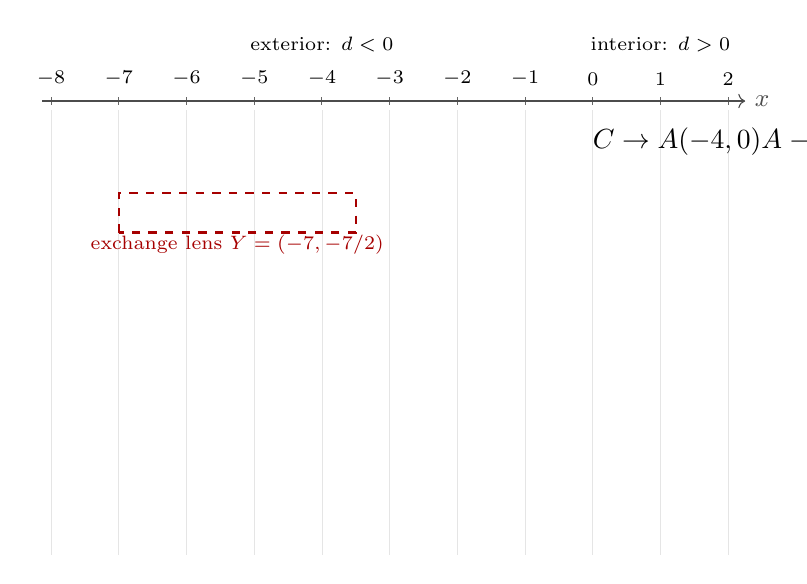
\begin{tikzpicture}[
  x=.86cm,y=1cm,
  bandA/.style={fill=orange!35,draw=black!35,line width=.3pt},
  bandB/.style={fill=cyan!28,draw=black!35,line width=.3pt},
  bandC/.style={fill=black!12,draw=black!35,line width=.3pt},
  lens/.style={draw=red!65!black,dashed,line width=.8pt}
]
  \foreach \geometrytick in {-8,-7,...,2} {
    \draw[black!10,line width=.3pt]
      (\geometrytick,.48) -- (\geometrytick,-5.17);
    \draw[black!60,line width=.35pt]
      (\geometrytick,.55) -- (\geometrytick,.65);
    \node[above,font=\scriptsize] at (\geometrytick,.67)
      {$\geometrytick$};
  }
  \draw[->,black!70] (-8.13,.60) -- (2.25,.60)
    node[right,font=\small] {$x$};
  \node[font=\scriptsize] at (-4,1.32) {exterior: $d<0$};
  \node[font=\scriptsize] at (1,1.32) {interior: $d>0$};

  \geometryrow{0}{\textbf{Main: initial}\\before the exchange}
  \geometryband{0}{-8}{0}{C}
  \geometryband{0}{0}{1}{A}
  \geometryband{0}{1}{2}{B}

  \geometryrow{-.82}{\textbf{Auxiliary}\\three nested births}
  \geometrybandat{-.82}{-8}{-6}{C}{-7.22}
  \geometryband{-.82}{-6}{-5}{B}
  \geometryband{-.82}{-5}{-4}{A}
  \geometrybandat{-.82}{-4}{-3}{C}{-3.72}
  \geometryband{-.82}{-3}{-2}{A}
  \geometryband{-.82}{-2}{-1}{B}
  \geometryband{-.82}{-1}{2}{C}
  \draw[lens] (-7,-1.07) rectangle (-3.5,-.57);
  \node[below,inner sep=0pt,font=\scriptsize,text=red!65!black] at (-5.25,-1.09)
    {exchange lens $Y=(-7,-7/2)$};

  \geometryrow{-1.64}{\textbf{Main: exchange}\\auxiliary retired}
  \geometryband{-1.64}{-8}{-6}{C}
  \geometryband{-1.64}{-6}{-5}{B}
  \geometryband{-1.64}{-5}{-4}{A}
  \geometryband{-1.64}{-4}{0}{C}
  \geometryband{-1.64}{0}{1}{A}
  \geometryband{-1.64}{1}{2}{B}

  \geometryrow{-2.46}{\textbf{Main: first death}\\$C\to A$ on $(-4,0)$}
  \geometryband{-2.46}{-8}{-6}{C}
  \geometryband{-2.46}{-6}{-5}{B}
  \geometryband{-2.46}{-5}{1}{A}
  \geometryband{-2.46}{1}{2}{B}

  \geometryrow{-3.28}{\textbf{Main: second death}\\$A\to B$ on $(-5,1)$}
  \geometryband{-3.28}{-8}{-6}{C}
  \geometryband{-3.28}{-6}{2}{B}

  \geometryrow{-4.10}{\textbf{Main: birth}\\$B\to C$ on $(-3,0)$}
  \geometryband{-4.10}{-8}{-6}{C}
  \geometryband{-4.10}{-6}{-3}{B}
  \geometryband{-4.10}{-3}{0}{C}
  \geometryband{-4.10}{0}{2}{B}

  \geometryrow{-4.92}{\textbf{Main: final death}\\$B\to C$ on $(-6,-3)$}
  \geometryband{-4.92}{-8}{0}{C}
  \geometryband{-4.92}{0}{2}{B}
\end{tikzpicture}
\endgroup
\caption{Normal-band words at one fixed $0<s<n$, in the coordinate
  $x=d/w(s)$ with $w(s)=10^{-3}\min(s,n-s)$; the chart displays only
  $-8\le x\le2$. The auxiliary starts uniformly at $C$ before the three
  nested births shown in its row. Exchanging the two sheets on the dashed
  lens creates the next main row: both displayed transverse boundaries
  lie in $C$ corridors on both sheets. The two deaths leave the interface
  at $x=-6$; the last
  birth and death move it to $x=0$, restoring the exterior label $C$.
  These are nominal labels: $A,B,C$ may coincide. This is a transverse
  schematic away from the edge endpoints and their point treatments.}
\label{fig:geometry-bands}
\end{figure}


Every band used in this sequence is contained in $-8<x<2$.  Such
bands along distinct edges of $S$ have disjoint interiors.  Opposite
edges are separated by $n$, whereas their bands have width at most
$0.004n$ on either relevant side.  For adjacent edges, a common point
in the parallel-coordinate spans would have to lie inside $S$ near
the shared corner.  If its two distances from those edges are $r_1,r_2$,
membership in both enlarged bands would imply
$r_1<0.008r_2$ and $r_2<0.008r_1$, which is impossible.  The negative
part of an edge band lies in its one exterior neighboring square, and
cannot enter the parallel-coordinate span of an adjacent edge.
Consequently an already completed edge does not alter the normal word
needed at the next one.  At the end of the four edge operations $S$
has label $B$ and every other square has its original label.  The same
description is valid along the placeholder exterior: all temporary
plane changes there are restored at the end.

\subsection{Uniform angular separation}

We record precisely the geometry needed to invoke the information
estimate.  For a given elementary operation let $\mathcal V$ be its
set of marked corners or endpoints and put
$d_{\mathcal V}(y)=\min_{v\in\mathcal V}\abs{y-v}_\infty$.
For a birth, its \emph{surrounding guide} is the guide before the
insertion; for a death, it is the guide after the removal.  In that
surrounding guide the changed region lies within a single label
$P_\circ$.

\begin{lemma}[Separation of the unmodified bands]
\label{lem:geometry-angular}
There is a fixed $a_0>0$ such that every unmodified elementary birth or
death above has changed region $R$ of diameter $O(n)$ and surrounding
guide $f$ satisfying
\begin{equation}
 \dist\bigl(y,\overline{\{f\ne P_\circ\}}\bigr)
 \ge a_0\min\{n,d_{\mathcal V}(y)\},
 \qquad y\in\overline R.
 \label{eq:geometry-birth-clearance}
\end{equation}
For an unmodified lens exchange, every point in the closure of the
positions that are not common $C$ on its two before guides satisfies
\begin{equation}
 \dist(y,\partial Y)
 \ge a_0\min\{n,d_{\mathcal V}(y)\}.
 \label{eq:geometry-exchange-clearance}
\end{equation}
Here and throughout this section distances are ambient sup distances.
\end{lemma}

\begin{proof}
For the central birth the closed changed region is separated from the
exterior of $S$ by the four edge bands, except at the four corners.
Near a corner its two distances from the adjacent edges are bounded
below by a fixed positive fraction of its sup distance from that
corner.  This gives the asserted conical separation there.  Away from
the corners the margin is a fixed positive fraction of $n$.

The first auxiliary insertion has a uniform surrounding guide.  The
second and third have closed normal intervals strictly inside the
surrounding intervals $(-6,-1)$ and $(-5,-2)$, respectively.  For the
first main death the surrounding $A$ interval is $(-5,1)$ and the
changed interval is $(-4,0)$.  For the second main death the surrounding
$B$ sector includes $(-6,2)$ and the changed interval is $(-5,1)$.
For the last birth the surrounding $B$ sector again includes
$(-6,2)$, while the inserted interval is $(-3,0)$.  For the last death
the surrounding $C$ sector includes $(-8,0)$ and the changed interval
is $(-6,-3)$.  All these margins are strict.  The enlarged edge bands
avoid unrelated edges and blocks by the preceding disjointness check.

For the exchange, the main guide is $C$ throughout the open exterior
band.  Both lens thresholds $-7$ and $-7/2$ lie strictly inside $C$
sectors of the auxiliary word in \eqref{eq:geometry-aux-word}.
Hence the lens boundary can meet the closed noncommon-$C$ region only
at its two marked endpoints.

In a fixed neighborhood of every marked point, in units of $n$, all
these interfaces are straight rays.  The relevant closed conical sets
have no common direction: away from their center they are disjoint by
the strict interval margins just checked.  Their intersections with a
unit sup sphere therefore have positive separation.  Homogeneity gives
\eqref{eq:geometry-birth-clearance} and
\eqref{eq:geometry-exchange-clearance} near the marked points.  On
the remaining bounded region, compactness after scaling by $n$ gives
a positive minimum separation.  Points far from the bounded lens are
harmless for \eqref{eq:geometry-exchange-clearance}.

Only finitely many scaled configurations occur: the baseline nearby
$n$-squares have a finite number of label-equality patterns, and the
band prescriptions are fixed.  Thus one $a_0$ works for all of them.
Identifying two nominal labels only removes parts of the obstructing
sets or makes an operation an identity, and never worsens a separation
already proved.  This includes equality with the single placeholder
label.
\end{proof}

All true vertices of an unmodified guide are separated on scale $n$.
Indeed the baseline vertices are grid corners.  The new band interfaces
are disjoint except at their indicated endpoints.  Their bends at
$s=n/2$ have only two incident labels and so are not true vertices.
In a fixed-radius neighborhood of a marked point, in units of $n$,
the only possible true vertex is the marked point itself.

\subsection{Point treatment and the actual bulk operations}

Before implementing one elementary birth or death, homogenize each
involved sheet inside the radius-$t$ square around every mark to its
surrounding label $P_\circ$.  Make the same modification in the target
guide of that elementary operation.  Thus its actual bulk recoloring
is truncated by those squares.  For an exchange, homogenize both
sheets there to $C$; the lens $Y$ itself need not be altered because
the assignments coincide throughout the homogenized portions.  After
the bulk operation, remove the point treatment by changing to the
specified target guide.  We prove below that every homogenization and
every removal is a small-patch rewrite.

Choose $K_0$ large enough that, when $n>K_0t$, the tenfold enlargements
of the treated squares are disjoint, contain no other unmodified true
vertices, and lie inside the straight-ray charts used above.  In a
treated neighborhood, any newly created true vertex is at the
intersection of a ray with the square rim.  The set of possible rim
intersection points is finite after scaling by $t$.  Coincident
points count as one point.  There is therefore a positive minimum
separation between distinct possible centers, uniformly over the
finite pattern family.  Take $\epsilon_0$ small compared with these
separations, with the ordinary grid separations, and with $a_0$.
This makes the outer holes disjoint, including in the temporary guides.

Figure~\ref{fig:geometry-points} illustrates how a true vertex can
move to the rim during a point treatment.
\begin{figure}[tbp]
\centering
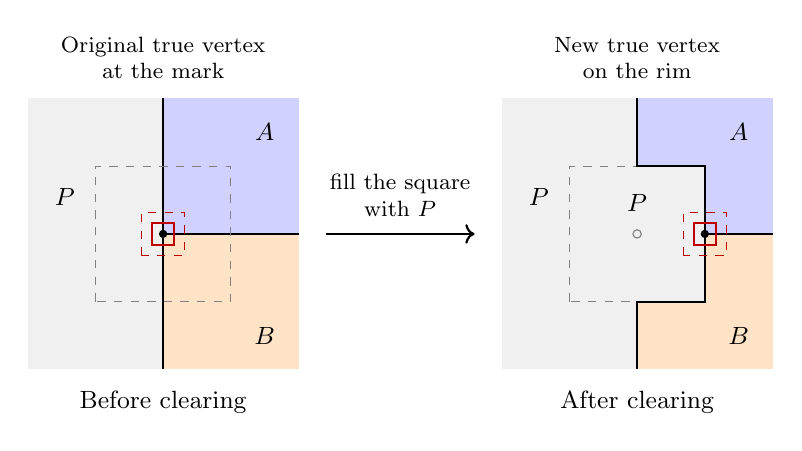
\begin{tikzpicture}[x=0.86cm,y=0.86cm,font=\small]
  \begin{scope}[shift={(-3.5,0)}]
    \fill[gray!12] (-2,-2) rectangle (2,2);
    \fill[blue!18] (0,0) rectangle (2,2);
    \fill[orange!22] (0,-2) rectangle (2,0);
    \draw[thick] (0,-2)--(0,2);
    \draw[thick] (0,0)--(2,0);
    \draw[dashed,gray] (-1,-1) rectangle (1,1);
    \draw[red!75!black,thick] (-0.16,-0.16) rectangle (0.16,0.16);
    \draw[red!75!black,dashed] (-0.32,-0.32) rectangle (0.32,0.32);
    \fill (0,0) circle (1.5pt);
    \node at (-1.45,0.55) {$P$};
    \node at (1.5,1.5) {$A$};
    \node at (1.5,-1.5) {$B$};
    \node[below] at (0,-2.18) {Before clearing};
    \node[above,align=center,font=\footnotesize] at (0,2.15)
      {Original true vertex\\at the mark};
  \end{scope}
  \draw[->,thick] (-1.1,0)--(1.1,0);
  \node[above,align=center,font=\footnotesize] at (0,0.12)
    {fill the square\\with $P$};
  \begin{scope}[shift={(3.5,0)}]
    \fill[gray!12] (-2,-2) rectangle (2,2);
    \fill[blue!18] (0,0) rectangle (2,2);
    \fill[orange!22] (0,-2) rectangle (2,0);
    \fill[gray!12] (-1,-1) rectangle (1,1);
    \draw[dashed,gray] (-1,-1) rectangle (1,1);
    \draw[thick] (0,2)--(0,1)--(1,1)--(1,-1)--(0,-1)--(0,-2);
    \draw[thick] (1,0)--(2,0);
    \draw[red!75!black,thick] (0.84,-0.16) rectangle (1.16,0.16);
    \draw[red!75!black,dashed] (0.68,-0.32) rectangle (1.32,0.32);
    \fill (1,0) circle (1.5pt);
    \draw[gray] (0,0) circle (1.5pt);
    \node at (-1.45,0.55) {$P$};
    \node at (0,0.45) {$P$};
    \node at (1.5,1.5) {$A$};
    \node at (1.5,-1.5) {$B$};
    \node[below] at (0,-2.18) {After clearing};
    \node[above,align=center,font=\footnotesize] at (0,2.15)
      {New true vertex\\on the rim};
  \end{scope}
\end{tikzpicture}
\caption{A point treatment for three distinct labels, shown in units of
$t$.  The dashed gray square is the radius-one treated square; solid
black lines are actual label interfaces.  After filling with $P$, the
only true vertex in this example is the meeting of $P,A,B$ on the right
rim.  The other ray/rim contacts involve only two labels.  Red solid
and dashed squares illustrate the inner and outer holes at the actual
true vertices, enlarged for visibility.  In the protocol their radii are
$h_n$ and $2h_n$, with one uniformly small $\epsilon_0$; the same
construction handles the finitely many ray patterns in the proof.}
\label{fig:geometry-points}
\end{figure}


For a birth or death, a point of the remaining closed changed region
lies outside the interiors of the treated squares.  Consequently
$d_{\mathcal V}(y)\ge t$, and homogenization to the surrounding label
can only remove its other-label obstructions.  By
\eqref{eq:geometry-birth-clearance}, after decreasing a fixed constant
if necessary, its separation from the other labels is bounded below by
\begin{equation}
 a_1\max\{t,\min(n,d_{\mathcal V}(y))\},
 \qquad a_1>0.
 \label{eq:geometry-floor}
\end{equation}
Every true vertex of the surrounding temporary guide belongs to the
closure of positions of labels different from $P_\circ$.  Enlarging
such a center to its outer hole square subtracts at most $2h_n$ from
this separation.  Since $h_n=\epsilon_0t$ in the present large-scale
case, a further fixed decrease of $a_1$ preserves
\eqref{eq:geometry-floor} for all outer hole sites too.

There are no changed true vertices in the bulk recoloring.  To see
this also at the treated rims, the closure of the truncated changed
region has a positive neighborhood containing only $P_\circ$ in the
surrounding guide.  A birth or reversed death introduces only one
additional label in that neighborhood.  Thus any newly drawn
interface, including where it meets a treated-square rim, has at most
two incident labels.  Existing true vertices are separated from this
closed change and retain their guides, holes, and tag holders.  The
raw target $T$ is therefore outside all holes, compactly located in
diameter $O(n)$, and satisfies the tapering hypothesis against the set
$E$ consisting of other owners and all outer hole sites.  The remaining
raw buffer has a single owner.  Lemma~\ref{lem:birth}, in its forward
or reverse form, implements the bulk change.

For the exchange, homogenization removes all noncommon-$C$ positions
inside the treated squares.  By
\eqref{eq:geometry-exchange-clearance}, every remaining such position
has the same floor at $t$ in its distance from $\partial Y$.  This
also holds for new rim vertices: a rim true vertex belongs to the
closure of an outside sector that is not $C$, and the original angular
estimate applies at that point.  Thus $\partial Y$, including each of
its intersections with a treated-square rim, lies in an open
common-$C$ corridor.  No new true vertex is created by exchanging
the guides along that boundary.

Every true vertex on either sheet belongs to the closure of a
noncommon-$C$ region.  Its distance from $\partial Y$ is at least a
fixed multiple of $t$ in a treated neighborhood, and obeys the larger
angular bound elsewhere.  The full outer hole square, of radius
$2\epsilon_0t$, therefore lies strictly on one side of the lens
boundary.  The same tapered bound holds at every point of an outer hole, not only
at its center: both $y\mapsto\dist(y,\partial Y)$ and
$y\mapsto d_{\mathcal V}(y)$ are $1$-Lipschitz. If $c$ is the center
and $|x-c|_\infty\le2\epsilon_0t$, put
$Q_x=\max\{t,\min(n,d_{\mathcal V}(x))\}$. A center clearance
$a_*\max\{t,\min(n,d_{\mathcal V}(c))\}$ gives
\[
 \dist(x,\partial Y)\ge a_*Q_x-2\epsilon_0(a_*+1)t
                   \ge \tfrac12a_*Q_x
\]
after fixing $\epsilon_0$ small enough. In particular, \emph{every}
selected variable-radius square in that hole lies on the same side,
since its radius is at most $2h_n$.  Exchanging a neighborhood of such a vertex substitutes one
complete sheet guide and carries its entire hole and tag.  It does
not splice sectors of two guides at a vertex.

For Lemma~\ref{lem:exchange}, let $T$ be the positions inside $Y$
that are not common $C$, together with all inside outer hole sites,
and let $E$ be the analogous set outside $Y$.  The set $T$ has
diameter $O(n)$.  Any segment from a point of $T$ to a point of $E$
crosses $\partial Y$, so its length is at least the distance of that
point of $T$ from the boundary.  The preceding clearance bounds,
including the outer-hole enlargement, therefore give the required
tapering separation of $T$ from $E$.  On the remaining positions both
raw copies are held by $C$.  This proves all hypotheses of the exchange
lemma, including its condition on whole holes and their tags.

All statements use actual labels.  Coalescing nominal labels cannot
create a meeting of three actual owners: the closure of an identified
region is the union of its finitely many former closures.  If a nominal
vertex disappears under such an identification, at most two actual
owners meet there and no vertex encoding is required.  The same
argument covers the exterior placeholder.  Empty physical targets
need no information estimate.

Choose one fixed $a>0$ smaller than all the surviving constants in
these tapering bounds.  Proposition~\ref{prop:angular}, at accuracy
$L^{-60}$, then supplies a sufficiently large fixed $D$ in
\eqref{eq:geometry-scales}.  The birth and exchange errors are
$O(L^{-30})$, as required by their lemmas.  The constants used to
choose $a$ depend only on the fixed geometric templates, not on $D$.

\subsection{The small-patch covers}

We verify every invocation of Lemma~\ref{lem:small-rewrite}.  The
following compactness observation makes the two-owner condition
uniform, including along the boundary of an inner hole.

Fix a compact working neighborhood and one scaled guide.  For each
actual label $c$, let $F_c$ be the closure of its region in that
neighborhood, with all open inner hole squares removed.  Each $F_c$
is compact.  No three $F_c$ with distinct actual labels have a common
point, because every true vertex lies strictly inside its own inner
hole.  It follows that there is a positive footprint diameter such
that no smaller footprint meets three of these sets.  Otherwise take
a sequence of shrinking footprints, pass to constant label choices
and convergent points in the compact working neighborhood, and obtain
a point common to three distinct $F_c$.

This remains uniform for our small-scale and resizing radius
parameters.  After scaling, these parameters range over compact
intervals bounded away from zero.  The joint sets of a parameter and
a point belonging to $F_c$ are closed: being outside an open square
is a non-strict distance inequality.  The same convergent-subsequence
argument applies to the joint sets.  There are only finitely many
label-equality types, so take the minimum positive footprint bound
over those types.  Apply the test separately to the old and new
guides, then take the smaller bound.  Different old and new hole
centers do not mix the two tests.

Notice that the \emph{center} of a footprint may lie inside a hole.
The condition counts labels only at footprint points outside the
relevant inner holes.  Thus this observation permits a net of small
patches to cover the \emph{whole outer} hole footprints, as required
by Lemma~\ref{lem:small-rewrite}.

\paragraph{Point homogenization and removal.}
For one mark in the large-scale case, work in its radius-$2t$
neighborhood.  Include as affected every old and new hole at the
marked center or on the treated-square rim.  These are all possible
changed true vertices, and their outer squares lie strictly inside
that neighborhood for small $\epsilon_0$.  There are no other holes
nearby.  In units of $t$, the old and new guides are from a finite
family of ray patterns, with or without the square clearing, and the
inner hole radius is $\epsilon_0$.

Choose a fixed sufficiently small $\nu>0$.  Patches with inner radius
$u=\nu t$, centered on a square net of mesh at most $u$, cover the
treated square and all affected outer holes.  Take the centers within
$u$ of the set to be covered.  With $\nu$ small, their outer squares
are still inside the working neighborhood and avoid every untouched
hole.  The compactness observation gives at most two old owners
outside the old inner holes and at most two new owners outside the
new inner holes in each outer patch.  The number of patches is fixed:
the working diameter is $O(t)$ and the patch radius is $\nu t$.
Their raw owners and affected tag holders are among the bounded list
of parties in this local diagram.  Apply
Lemma~\ref{lem:small-rewrite}, one mark and one sheet at a time.
The separated marked neighborhoods do not change one another's
diagrams.  The same verification applies when removing the point
treatment after the bulk operation, using its actual target guide.

\paragraph{Direct repainting when $n\le K_0t$.}
Before and after a direct repainting, true vertices are grid corners.
Only the four corners of the square being repainted can change their
true-vertex status or their tag holder.  Treat every old or new hole
at those corners as affected.  The hole radius obeys
\begin{equation}
 \frac{\epsilon_0}{\max(K_0,1)}
 \le \frac{h_n}{n}\le\epsilon_0.
 \label{eq:geometry-small-radius}
\end{equation}
In units of $n$, the old/new label patterns form a finite collection,
and the possible radius ratios lie in the displayed compact positive
interval.  The compactness observation gives a uniform sufficiently
small patch radius $u=\nu n$.  A fine net covers $S$ and the entire
affected outer holes with a fixed number of such patches.  Every
untouched grid-corner hole is a fixed scaled distance from the set to
be covered: corners of $S$ have all been included, and any other grid
corner is at distance at least $n$ from $S$.  Choosing $\epsilon_0$
and then $\nu$ small makes all outer patches avoid those holes.  All
hypotheses of Lemma~\ref{lem:small-rewrite} follow.  This
directly repaints $S$ without using an auxiliary sheet.

\paragraph{Hole resizing.}
Entering level $n$, the old and new radii are
$\epsilon_0\min(2n,t)$ and $\epsilon_0\min(n,t)$.  If they differ,
then $n<t$, in particular $n\le K_0t$, and their ratio lies between
one and two.  The current guide is unchanged and is uniform on
$2n$-blocks.  Resize one true-vertex hole at a time.  The union of
its two outer footprints has diameter $O(n)$; other true vertices
are separated on that scale.  The same compactness and fine-net
argument covers both footprints, avoids all other holes, and gives
the separate old/new two-owner tests.  Intermediate configurations
with some holes already resized obey the same positive radius and
separation bounds.  This proves the required small-patch rewrite for
each resize.

For completeness, these covers apply uniformly to every selected
adaptive radius in a rewrite branch.  A selected patch square
contains its inner square, so every changed raw site and every site
of an affected selected hole is intercepted by a patch.  A raw
input-to-output identity wire that remains unintercepted cannot
change owner.  An old-hole decoded ket therefore has no open leg
directly at a new raw output, and a new-hole encoding bra has none
directly at an old raw input.  Overlapping patches merely connect an
earlier patch ket to a later patch bra.  Open patch-bra legs come
from raw inputs outside all old inner holes, and open patch-ket legs
go to raw outputs outside all new inner holes.  Their owner counts
are exactly the separate two-owner counts just proved.  Thus the
geometric hypotheses give the branchwise support facts used in the
tensor expansion of Lemma~\ref{lem:small-rewrite}, even when old
and new holes have different radii.

There is no circular choice of constants.  First fix the band
templates and obtain $a_0$ and their radial-chart constants; then
choose $K_0$, then $\epsilon_0$, and then the fixed mesh parameter
$\nu$ from the compact families just described.  Choose the smaller
clearance $a$ and the information scale constant $D$ afterward.
Finally choose $B_0$ large enough that all hole radii and all added
patch radii are at most $B_0\log L$.  A fixed multiple of $K_0D$
suffices, since the point patches have size $O(t)$, the direct
patches have size $O(n)\le O(K_0t)$, and all holes have size $O(t)$.
The adaptive patch ranks may depend on this fixed $B_0$, but every
selected support still lies between its predetermined inner and
outer square, so no geometric constant has to be chosen again.

\subsection{Party lifetimes and the protocol bounds}

Each elementary birth, death, or exchange has a fixed number of
marks.  The point treatments have a fixed number of patches and
parties.  The edge word uses a fixed number of elementary operations
and four auxiliary sheets at most per repainting.  Consequently each
repainting, and each junction resize, uses a uniformly bounded
number of linked gates and parties.  Small-patch rewrites can be
replaced by arbitrarily accurate polynomial expansions and rescaled
near one to remain contractions.  Together with the $L^{-60}$ patch
tests and the $O(L^{-30})$ splitting errors, choose their precision
so that each change has reference-vector error at most $C L^{-20}$.

At a level-$n$ repainting, every active main owner is an $n$- or
$2n$-block owner.  On the affected footprints those blocks lie at
distance $O(n)$ from the repainted square.  The same is true of
their tag holders, since tags are held by incident labels.  An
auxiliary uses only the labels of the local edge and point diagrams;
its uniform initial owner $C$ is the actual neighboring-block owner,
even though it privately holds a whole copy of $\Omega$.  The
placeholder party is attached to the repainted block at scale $n$.
Resizing uses the current block labels near its junction.  Private
buffer isometries may act on registers at much more distant physical
positions, but create no additional party or link.

The following stronger invariant concerns active main owners; the
inactive exterior placeholder is omitted at the start and end of a
level. It proves the lifetime claim, rather than just locality at an
individual step:
\begin{equation}
 \begin{aligned}
  \text{start of level }n &: \text{ only }2n\text{-block main labels};\\
  \text{during level }n &: \text{ only }2n\text{- and }n\text{-block main labels,
       plus its temporary placeholder};\\
  \text{end of level }n &: \text{ only }n\text{-block main labels}.
 \end{aligned}
 \label{eq:geometry-active-labels}
\end{equation}
Main tags always use incident non-placeholder labels.  Hence a party
of side $m$ disappears from every main tag as well as every main
guide region by the end of level $m/2$.  In particular, when the last
incident child square repaints, its corner rewrite updates the tag
at that junction.  Resizing introduces no obsolete owner.  Thus
this party can occur in linked gates only at levels $m$ and $m/2$
and their intervening transition.  At these scales there are only
a fixed number of repaintings or junctions within distance $O(m)$
of its block.

Frozen auxiliary frames do not invalidate this invariant.  Each is
initialized, used in its one edge construction, returned from its
point treatment to its specified final frame, and permanently
retired before the repainting ends.  Its remaining entangled
registers and tags are kept idle at their owners.  No subsequent
gate undoes that exchange, and no later auxiliary initialization
consults a frozen label: its $C$ is always selected from the current
main guide.  Therefore frozen memory contributes no further linked
incidence.  The same applies to a retired placeholder party.  A
fresh placeholder identity at the next repainting has no raw main
register or persistent main tag to inherit.  This proves a uniform
bound on every party's total linked participation.

For later routing, a square of side $n=2^j$ and block indices $(r,s)$
has the integer address
\begin{equation}
 a(S)=
 \begin{cases}
 (nr+n/2,\,ns+n/2),&j\ge1,\\
 (r,s),&j=0.
 \end{cases}
 \label{eq:geometry-addresses}
\end{equation}
Use the same address for its additional parties.  The preceding
locality statement gives $O(n)$ address distances for parties sharing
a gate, and their scales are equal or adjacent.  The addresses lie
in $\{0,\ldots,N-1\}^2$; unit-square physical outputs have their
actual site indices as addresses.

There are $O((N/n)^2)$ repaintings and junctions at scale $n$.
Summing over dyadic scales gives $O(N^2)=O(L^2)$ in total.  The number
of block parties, additional parties, auxiliary sheets, and changes
is therefore $O(L^2)$, and in particular bounded by $C L^3$.
Each frozen auxiliary has only a fixed number of holes: its guide
differs from its uniform guide only in one bounded edge template and
its endpoint treatments.  Even the weaker total bound $C L^3$ on
frozen auxiliary holes will suffice.

Initialize all required copies of $\Omega$ privately at their future
owners, including the main copy at the root.  This is a pure product
initialization across parties, with no restriction on private state
complexity.  At the beginning the main guide has only the root label
and the exterior placeholder, so it has no true vertex and no hole.
At every stage use the tensor product of the designated main frame,
active auxiliary frames, idle initial copies, and frozen final
auxiliary frames as its reference vector.  Untouched factors have
norm at most one, so the local reference-error bounds remain valid
with all these spectators.

At level $n=1$, choose $\epsilon_0<1/4$.  A grid-corner outer hole
then has radius $2\epsilon_0<1/2$ and contains no cell-center physical
site.  Its encoding is trivial.  Thus all remaining main registers
are raw at their unit-square parties and the main reference is
exactly $\Omega$, apart from trivial tags.  The other reference
factors comprise $\Xi$.  Each encoded auxiliary frame has norm at
least one minus its number of holes times $L^{-60}$, by the frame
constraint and contraction bounds.  Multiplying these lower bounds
and using the total frozen-hole count gives
$1-C L^{3-60}\le\norm{\Xi}\le1$.  All auxiliary registers and all
nonphysical outputs can be discarded party by party.

This proves every assertion of Proposition~\ref{prop:protocol}.

\section{From the protocol to a PEPS}\label{sec:assembly}

We now turn the distributed construction into the vector approximation of
Theorem~\ref{thm:main}. All private registers, including frozen sheets and
effect inventories, are kept until the last trace. This preserves the
normalization information needed when passing from an operator network
to a ket.

\subsection{Error and normalization}

Apply Proposition~\ref{prop:protocol} with patch and information power $60$.
The initial state is a product \emph{by party}: the root privately holds
the main $\Omega$, and every future auxiliary copy of $\Omega$ is held
privately by its designated initializing party. Private dimensions and
initial vectors are unrestricted in Theorem~\ref{thm:compression}.
The main initial guide has one label and needs no holes.

There are at most $CL^3$ changes and at most $CL^3$ holes across all frozen
auxiliary reference frames. Each encoding is contractive, and its failure
on $\Omega$ is at most the number of its holes times $L^{-60}$. Thus the
final reference vector has the form
\begin{equation}\label{eq:reference-junk}
 \Omega\otimes\Xi,
 \qquad 1-CL^{-57}\le\norm{\Xi}\le1.
\end{equation}
At unit scale all physical outputs are raw at their unit parties; any
remaining main hole has empty physical support and a trivial tag.

Instantiate the protocol using the contractive polynomial approximants
of Lemma~\ref{lem:small-rewrite}, with operator-norm error at most
$L^{-25}$, for every small-patch rewrite.  The birth, death, and exchange
maps already have the required form.  Each selected change therefore takes
its reference vector within $O(L^{-20})$ of the next one, and the actual
protocol uses these selected contractions throughout.  Telescoping a
product of contractions bounds the accumulated vector error by the sum
of the individual errors. Consequently the actual final vector $\Psi$
satisfies
\[
 \norm{\Psi-\Omega\otimes\Xi}\le CL^{-17},\qquad \norm{\Psi}\le1.
\]
For vectors of norm at most one,
$\norm{|u\rangle\langle u|-|v\rangle\langle v|}_1
\le2\norm{u-v}$. Tracing the private outputs and using
\eqref{eq:reference-junk} gives
\begin{equation}\label{eq:protocol-density}
 \left\|\Tr_{\rm private}|\Psi\rangle\langle\Psi|
             -|\Omega\rangle\langle\Omega|\right\|_1
 \le CL^{-17}+CL^{-57}\le CL^{-10}.
\end{equation}
In particular the protocol does not rely on renormalizing an
exponentially small success amplitude.

Every party has physical output dimension at most $q$, every linked gate
has the expansion required in Theorem~\ref{thm:compression}, and linked
incidence is bounded over the whole lifetime of each party.
That theorem, with accuracy $L^{-5}$, therefore gives a party operator
network $\sigma$ with polynomial link dimensions and
\begin{equation}\label{eq:compressed-density}
 \norm{\sigma-|\Omega\rangle\langle\Omega|}_1\le CL^{-5}.
\end{equation}
The network has only boundedly many links per party, between parties
participating in the same local change. The sampling need not make
$\sigma$ positive or Hermitian.

\subsection{Extracting one ket column}

\begin{lemma}\label{lem:columns}
Let $\Omega$ be a unit vector on a tensor product of finite-dimensional
spaces. If an operator $\sigma$ satisfies
$\norm{\sigma-|\Omega\rangle\langle\Omega|}_1\le\eta<1$, then some
product-basis column $v=\sigma|z\rangle$ is nonzero and satisfies
\[
 \min_\theta\left\|\frac{v}{\norm v}-e^{i\theta}\Omega\right\|
 \le2\eta.
\]
Fixing this column in an operator tensor network leaves all its virtual
dimensions unchanged.
\end{lemma}
\begin{proof}
Put $E=\sigma-|\Omega\rangle\langle\Omega|$ and
$a_z=\langle\Omega|z\rangle$. Then
\[
 \sum_z\norm{E|z\rangle}^2=\norm E_2^2\le\eta^2,
 \qquad \sum_z|a_z|^2=1.
\]
Thus at least one $z$ with $a_z\ne0$ obeys
$\norm{E|z\rangle}\le\eta|a_z|$. For this $z$,
$w=v/a_z$ satisfies $\norm{w-\Omega}\le\eta$, so $w\ne0$ and
$|\norm w-1|\le\eta$. It follows that
$\norm{w/\norm w-\Omega}\le2\eta$.
Fixing the input basis index separately in each physical tensor selects
the same column without altering a virtual leg. No lower bound on
$|a_z|$ and no positivity assumption on $\sigma$ are used.
\end{proof}

For sufficiently large $L$, the bound $CL^{-5}$ is less than one, so
Lemma~\ref{lem:columns} applies to \eqref{eq:compressed-density}. We obtain a
nonzero ket network on the party graph with normalized error at most
$CL^{-5}$. It remains to realize that graph on the prescribed grid.

\subsection{Constant congestion on dyadic anchors}

Let $N$ be the least power of two with $N\ge L$, so $N<2L$.
Shift genuine lattice coordinates to $\{0,\ldots,L-1\}^2$ and work first
on the padded grid $\{0,\ldots,N-1\}^2$. A dyadic block of side $n=2^j$
with block indices $(r,s)$ has anchor
\begin{equation}\label{eq:anchors}
 a_{j,r,s}=\begin{cases}
 (2^jr+2^{j-1},\,2^js+2^{j-1}),&j\ge1,\\
 (r,s),&j=0.
 \end{cases}
\end{equation}
Temporary parties use the anchor of their creating block; only boundedly
many are attached to any block. All anchors lie on the padded grid.

The scale-separated network-to-PEPS embedding has a precedent in
Barthel--Kliesch--Eisert \cite[Section~III.C, Eqs.~(7)--(12)]{BarthelKlieschEisert2010}.
The proof below gives the routing for the present bounded-lifetime
network with polynomial link dimensions and treats finite-square
boundary folding explicitly.

\begin{lemma}\label{lem:routing}
The links of the party network can be routed on the padded grid with
constant edge congestion. After reflection into the genuine $L\times L$
grid, congestion is still constant and physical output coordinates are
unchanged.
\end{lemma}
\begin{proof}
Orient each link arbitrarily. Route it horizontally from the first
anchor, then vertically to the second. Proposition~\ref{prop:protocol}
ensures that the endpoint scales are equal or adjacent and their
separation is at most a fixed multiple of either scale.

A horizontal segment whose first endpoint has scale $2^j$, $j\ge1$,
lies on row
$y=2^{j-1}(2s+1)$. The exact two-adic valuation of $y$ is $j-1$; in
particular such a row is nonzero and determines a unique nonunit scale.
For a fixed horizontal edge on that row, only boundedly many anchors of
that scale can be within the allowed horizontal travel distance, since
successive anchors are $2^j$ apart. Each anchor carries boundedly many
parties of bounded degree. This gives a constant horizontal congestion.
Scale $j=0$ adds a separate constant, because its links have bounded
length. For vertical segments the same argument uses the column of the
second endpoint and its scale. Crossings are permitted: a grid-vertex
tensor carries all crossing virtual indices independently.

Define on padded coordinates
\[
 f(x)=\begin{cases}
 x,&0\le x\le L-1,\\
 2(L-1)-x,&L\le x\le N-1.
 \end{cases}
\]
Because $N<2L$, its values lie in $\{0,\ldots,L-1\}$.
Adjacent coordinates map to adjacent coordinates. Every coordinate and
every one-dimensional edge has at most two preimages. Hence each
horizontal or vertical edge of the physical square has at most four
padded edge preimages, counting repeated traversals of folded paths.
The congestion increases by at most four. The map fixes genuine output
coordinates. Zero-length links and coincident party tensors are contracted
locally.
\end{proof}

Each continued path carries an identity tensor on its virtual index.
At a crossing, take the product of the continuing index factors and any
party tensors located there. Group all indices traversing a grid edge
into a tensor-product index. If each original link has dimension at most
$C_1L^r$ and congestion is at most $\chi$, the new edge dimensions are at
most
\begin{equation}\label{eq:final-bond}
 (C_1L^r)^\chi.
\end{equation}
The single tensor at a genuine vertex, including its physical output,
is exactly an arbitrary map of the PEPS convention in
Theorem~\ref{thm:main}. Vertices without additional operations contribute
the requisite identity factors. Thus the ket network is a PEPS on the
same physical square.

\subsection{Order of constants and small sizes}

For completeness, the following order makes every uniformity assertion
explicit. Fix $q,J,\Delta$, the numerical error powers, and the exponents
used by the rectangular recursion. The finite band templates determine
their conical clearances. Choose the large point-treatment factor, then
the small hole fraction and the finite patch mesh. Choose a residual
clearance $a>0$, and then choose $D$ from
Proposition~\ref{prop:angular} at information power $60$.
The largest patch scale constant $B_0$ is selected afterwards to cover
all patches of scale at most a fixed multiple of $D\log L$.

Proposition~\ref{prop:patch} then determines a fixed rank exponent.
Only boundedly many such cylinder expansions occur in a change, so their
total branch count is polynomial. Choose the singular-subspace dimensions
in Lemma~\ref{lem:small-rewrite} next, to obtain operator error
$L^{-25}$. Choose the effect-inventory stack lengths from the
\emph{original} weighted expansion error in Lemma~\ref{lem:effects};
only afterwards expand the permutation averages. Finally choose the
Gaussian sample count in Theorem~\ref{thm:compression}. None of these
algebraic choices changes an earlier geometric support or clearance.
The resulting $C_1,r$ and the congestion $\chi$ in
\eqref{eq:final-bond} depend only on the fixed parameters and templates.

Increase a fixed threshold $L_0$ so that every preceding asymptotic
inequality holds and the error $CL^{-5}$ is at most $L^{-1}$ for
$L\ge L_0$. For the finitely many smaller sizes, every vector has an exact
PEPS on a spanning tree of the square grid. One explicit construction
uses a common index for the $q^{L^2}$ product-basis configurations on all
tree edges, equality tensors at tree vertices that also output the local basis state
of that common configuration, and puts each expansion coefficient at one
chosen root. Non-tree edges have dimension one.
This bond bound is finite and independent of the Hamiltonian at each
fixed $L$. Enlarging the single prefactor $C$ handles all $2\le L<L_0$.
Equation~\eqref{eq:final-bond} and Lemma~\ref{lem:columns} now prove
Theorem~\ref{thm:main} for every $L$.

\appendix
\section{Exact interfaces with the area-law companion}
\label{app:companion}

The companion \cite{RepoAreaLaw}, \emph{A two-dimensional area law from a
global spectral gap}, is used on the original ground state $\Omega$.
This appendix records the hypotheses and the division of work between the
two articles. A subregion is always a subsystem of that state; it is never
assigned a new gap assumption.

\paragraph{Hamiltonians, metrics, and entropy.}
The companion permits any finite induced domain $\Gamma\subset\mathbb Z^2$
with local dimension $q$ and one Hermitian term $h_X$ of norm at most $J$
for each nonempty support of induced-graph diameter at most a fixed $R$.
It assumes a unique unit ground vector and
$H-E_0I\ge\Delta(I-|\Omega\rangle\langle\Omega|)$.
Constants depend on $q,R,J,\Delta$ and explicitly fixed auxiliary
parameters, uniformly in the domain and Hamiltonian. All entropy logarithms
are natural. Its Theorem~1.1 and Corollary~1.2 give the area inequality
stated in Proposition~\ref{prop:area-law}. Here $\Gamma=\Lambda_L$ and
$R=1$, exactly covering \eqref{eq:model}.

\paragraph{Positive replacement.}
The Proposition ``Positive replacement of the Hamiltonian'' in
\cite[Section~4]{RepoAreaLaw} gives, for every fixed integer $k\ge1$ and
$\alpha=k/(k+1)$, positive contractions $k_i$ at the original interaction
anchors, of uniformly bounded anchor multiplicity, satisfying
\[
 k_i\Omega=0,\qquad
 \sum_i k_i\ge c_*^{-1}(H-E_0I)\ge(\Delta/c_*)(I-|\Omega\rangle\langle\Omega|),
 \qquad
 \|k_i-\mathbb E_{N_r(a_i)}k_i\|\le C e^{-cr^\alpha}.
\]
Here $\mathbb E_{N_r(a_i)}$ is conditional expectation onto the induced-graph
ball, for every integer $r\ge0$; $c_*,C,c$ may depend on $k$ and the fixed physical parameters. This
input underlies the companion amplification. It does not replace the
original Hamiltonian by a finite-range frustration-free Hamiltonian.

\paragraph{Templates, collars, and amplification.}
Definition ``A template'' and Proposition ``A sublinear collar bound'' in
\cite[Section~9]{RepoAreaLaw} use a cut $A\subseteq\Gamma$, its crossing-edge
endpoints $Z_A$, and a nonempty ambient lattice set
\[
 T=\bigcup_{a=1}^{N_0}(P_a\cap\mathbb Z^2),\qquad
 n\ge C_{\rm tpl}N_0(s_0+1),\quad \diam_\infty T\le n,
 \quad \dist_\infty(T,Z_A)>4D_0s_0.
\]
The $P_a$ are closed convex rectangles or triangles of sup diameter at most
$s_0$, with side slopes $0,\infty,1,-1$; $n,s_0$ are positive integers and
$s_0\ge1$. With $\epsilon=10^{-5}$, set
$\ell=\lfloor n^{1-\epsilon}\rfloor\le s_0$,
$T_\ell=T+[-\ell,\ell]^2_{\mathbb Z}$, $X=A\cap T$,
$S_0=A\cap T_\ell$, and $Y=S_0\setminus X$.
At all sufficiently large scales the input guarantees
\[
 I_\Omega(X:\Gamma\setminus S_0)\le Cn^{1-\epsilon},\qquad
 |S_0|\le Cn^2,\qquad
 |\partial_\Gamma X|,|\partial_\Gamma Y|,|\partial_\Gamma S_0|\le Cn.
\]

The Proposition ``Amplification'' in \cite[Section~10]{RepoAreaLaw}
requires these three bounds with any fixed common constant $C_0$ and
$\alpha=k/(k+1)>1-10^{-6}$. Put $\beta_0=1-2\cdot10^{-6}$.
For every fixed integer $M\ge1$ it supplies a radius
\[
 r\le C_M n^{(1-\epsilon)/\alpha},\qquad
 \ell+2r=o(n^{\beta_0}),\qquad
 I_\Omega(X':E)\le C_M n^{-M}
\]
simultaneously for every $X'\subseteq X$ and
$E\subseteq\Gamma\setminus N_{2r}(S_0)$. The radius and constants are
independent of the remote set and total volume. If also
$\dist_\infty(T,Z_A)>\ell+n^{\beta_0}$, then
$N_{2r}(S_0)\subseteq A$. In Proposition~\ref{prop:coarse} we take
$A=\Lambda$, so $Z_A=\varnothing$, choose $s_0,n$ comparable to the target
scale with fixed ratios, and use $M=1$. A graph neighborhood lies in the
corresponding ambient enlargement; this is the precise conversion used to
obtain the ambient-separation statement.

\paragraph{The two-family interface and its adaptation.}
The Lemma ``Two-family entropy cancellation'' in
\cite[Section~11]{RepoAreaLaw} states that, for a pure state and a partition
$A=D\mathbin{\dot\cup}\bigcup_iX_i$ into two ordered families, bounds
\[
 I\left(X_i:A^c\cup\bigcup_{j<i,\,f_j=f_i}X_j\right)\le\delta_i
 \quad(f_i\in\{0,1\})
 \quad\Longrightarrow\quad
 S(A)\le S(D)+\tfrac12\sum_i\delta_i.
\]
Its Proposition ``Two families with separated birth templates'' constructs
such regions for every cut with $b=|\partial_\Gamma A|>0$ and any fixed lower
scale $n_*$. It gives $|D|\le Cb$, $X_i\subseteq A\cap T_i$, admissible
separated templates with $n_i\ge n_*$ and
$\lfloor n_i^{1-\epsilon}\rfloor\le s_i$, and
\[
 \dist_\infty(T_i,Z_A)>2n_i^{\beta_0},\qquad
 \dist_\infty\left(T_i,\bigcup_{j<i,\,f_j=f_i}X_j\right)>2n_i^{\beta_0},
 \qquad \sum_i n_i^{-100}\le Cb.
\]
The constant may depend on $n_*$ and the template constants but not on the
cut or domain. These statements are used within the companion's area-law
proof. Lemma~\ref{lem:cell-cmi} adapts their ordering principle to a cell
with arbitrary exterior conditioning and proves that local variant in
full. In particular, we do not infer a conditional-information bound merely
by conditioning an ordinary mutual-information inequality.

The companion's replica limit is taken at each fixed finite physical
instance and schedule, before the geometric scale tends to infinity.
Its exported bounds concern the original one-copy state with the uniform
constants above. The later tapering construction, adaptive patch
constraints, density compression, encoded protocol, and routing are proved
in this article.

\begingroup
\small
\let\originalthebibliography\thebibliography
\renewcommand{\thebibliography}[1]{%
  \originalthebibliography{#1}%
  \addcontentsline{toc}{section}{\refname}%
}
\bibliographystyle{plain}
\bibliography{references}
\endgroup
\end{document}
